\chapter[Introdução]{Introdução}

\section{\textit{Considerações Iniciais}}

Neste Capítulo inicial apresenta-se o contexto no qual se insere este trabalho, as
justificativas que motivaram o desenvolvimento, o problema, o objetivo, a
metodologia de pesquisa adotada e a organização do trabalho nos capítulos seguintes.

\section{\textit{Contexto}}

Atualmente vivemos em uma era onde o mundo está cada vez mais dependente de software. Ele está tão acoplado nas mais diversas áreas que seria difícil prever como o mundo seria sem o suporte e as facilidades que ele traz ao nosso dia a dia. Diante deste acoplamento tão grande e do seu enorme crescimento nos últimos anos, consequência do avanço tecnológico, se torna cada vez mais importante desenvolver software. O desenvolvimento de software pode se inserir em diferentes contextos de negócio, e com isso diferentes habilidades são exigidas dos desenvolvedores, já que cada contexto possui suas particularidades. Além disso, o ritmo acelerado do mundo moderno faz com que os contextos evoluam, e com isso as suas atividades e necessidades (requisitos) também evoluam. A mudança nos requisitos, a sua diversidade, e em alguns casos a dificuldade em definí-los, leva o desenvolvimento tradicional de software a ser lento e caro em contextos que estão sempre evoluindo \cite{lieberman2006}. Além disso, a limitação na capacidade de produção de software de uma organização pode levar à priorização das demandas, e como consequência algumas áreas de negócio podem ficar sem atendimento. Neste contexto, se torna cada vez mais comum, aplicações de software serem desenvolvidas por desenvolvedores não profissionais, pessoas que não possuem conhecimento elevado em programação, mas que possuem expertise no domínio de negócio em que estão inseridas. O desejo de suportar seus objetivos neste domínio através de uma solução computacional, os leva a serem tanto desenvolvedores quanto usuários finais do software \cite{lieberman2006}.

Um relatório divulgado pelo \textit{Gartner} em Julho de 2011, indicou que desenvolvedores não profissionais iriam construir ao menos 25 \% das novas aplicações de negócio em 2014 \cite{paterno2013}. Portanto um modelo de desenvolvimento de software centrado nesses usuários finais, que desenvolvem cada vez mais sistemas e aplicações, vem ganhando força. O \textit{End User Development} - EUD tem como objetivo oferecer meios para que os usuários finais, que não são especialistas em programação, possam desenvolver aplicações de software. O EUD pode ajudar a aumentar a capacidade produtiva do departamento de TI de uma organização, bem como reduzir custos com o desenvolvimento de aplicações de negócio.

O serviço público brasileiro, por ter natureza administrativa, apresenta grande demanda por desenvolvimento de software. Porém, a limitada capacidade produtiva da área de TI e o excesso de burocracia para o aumento da mesma, que é feita através de concursos ou de contratos terceirizados, acaba contribuindo para que as demandas das áreas de negócio consideradas menos prioritárias sejam deixadas de lado \cite{artigoTcuGovTI}. O uso de planilhas e o desenvolvimento de aplicações clandestinas sem nenhuma documentação e padrão, por essas unidades de negócio, promove o desconhecimento de soluções informatizadas por parte da alta cúpula, bem como a duplicidade de esforços pelas unidades \cite{slideTCU}. Nesse sentido, alguns órgãos da administração pública federal vêm reconhecendo esses esforços feitos informalmente pelas áreas de negócio, e começaram a adotar o modelo EUD, com algumas adaptações, para tentar contornar os problemas relatados. Um dos órgãos pioneiros nessa adaptação, denominado de órgão público de estudo para fins de privacidade, passou a chama-la de modelo de desenvolvimento descentralizado, uma espécie de EUD onde as aplicações podem ser desenvolvidas por usuários ou por estagiários que os apóiam.

\section{\textit{Problema}}

O principal problema identificado está relacionado à maneira em que o desenvolvimento de sistemas descentralizados é executado no órgão público de estudo. Uma vez que os sistemas são desenvolvidos de forma descentralizada, ou seja, os departamentos realizam o desenvolvimento de seus sistemas conforme suas necessidades, eles geralmente acabam negligenciando o uso de boas práticas e de padrões de desenvolvimento.

Outro problema que é inerente ao desenvolvimento descentralizado é que as entregas que contenham erros podem trazer prejuízos ao órgão. O desenvolvimento descentralizado tem particularidades que são diferentes do desenvolvimento de software tradicional, como o uso de soluções improvisadas, o usuário final não tem tempo nem conhecimento para construir soluções tão sólidas e duradouras como um desenvolvimento profissional.

Assim a questão de pesquisa abordada nesse trabalho é:
\begin{itemize}
\item Como apoiar o desenvolvedor na construção de sistemas descentralizados para promover a qualidade e manutenibilidade destes sistemas?
\end{itemize}

\section{\textit{Objetivos}}

Dentro deste contexto, o objetivo geral deste trabalho é desenvolver uma solução de apoio ao desenvolvimento descentralizado no órgão público de estudo, agregando recursos que promovam a qualidade dos sistemas desenvolvidos, a partir de princípios e conceitos de engenharia de software.

\begin{comment}
%TODO: Melhorar os objetivos específicos.
\end{comment}
Considerando o objetivo geral, foram definidos os seguintes objetivos específicos:

\begin{enumerate}
	\item Entender o contexto do desenvolvimento EUD no órgão público alvo;
	\item Diagnosticar os problemas no desenvolvimento EUD de aplicações;
    \item Obter um modelo de solução;
	%\item Selecionar as práticas da engenharia de software que sejam adequadas à solução dos problemas encontrados e ao contexto.
	%\item Elaborar o modelo conceitual da solução de apoio.
	%\item Construir a solução de apoio.
	%\item Selecionar um projeto para a aplicação da solução.
	%\item Aplicar a solução de apoio no projeto selecionado.
	%\item Relatar os resultados obtidos através de um modelo.
\end{enumerate}


\begin{comment}
Apesar disso, existem ainda algumas dificuldades no desenvolvimento por parte dos estagiários desenvolvedores, como a falta de padronização e o que demonstra a necessidade de a elaboração de um processo embasado por princípios em conceitos da engenharia de software, ao mesmo tempo que não seja custoso aos desenvolvedores, já que iria contra a flexibilidade que preconiza o modelo EUD.

\citeonline{lieberman2006} relatou que um dos objetivos da interação humano-computador, além de desenvolver sistemas que são fáceis de usar, seria desenvolver sistemas que são fáceis de desenvolver.
\end{comment}

\section{\textit{Justificativa}}

A falta de padrões e adesão a boas práticas no desenvolvimento de aplicações pode levar à problemas relacionados a qualidade e manutenibilidade destas aplicações. Segundo \cite{blackwell2003notational}, no caso do uso de ferramentas de programação, é muito fácil para os desenvolvedores profissionais de software assumir que qualquer pessoa irá se aproximar ao seu nível profissional de programação. A fim de evitar esta armadilha, são necessários atenção e investigação especializada para os usuários finais por parte dos desenvolvedores profissionais, durante a criação de novas tecnologias voltadas ao EUD. Baseado nesses argumentos, é necessário que os desenvolvedores EUD tenham uma atenção especial para o desenvolvimento de seus sistemas, através de um modelo que lhes dê suporte.

\section{\textit{Metodologia}}

A escolha da estratégia de pesquisa deve satisfazer três condições: o tipo de questão de pesquisa, o controle que o pesquisador possui sobre os eventos comportamentais efetivos e o foco em fenômenos históricos, em oposição a fenômenos contemporâneos \cite{yin2001estudo}.

Levando em consideração essas condições, a metodologia de pesquisa deste trabalho foi classificada quanto à abordagem, natureza, objetivos ou tipologia, procedimentos técnicos e as técnicas de coleta de dados.

Quanto à abordagem, é classificada como qualitativa, uma vez que as pesquisas
classificadas como qualitativas estão relacionadas ao levantamento de dados sobre as motivações de um grupo em compreender e interpretar determinados comportamentos, e em obter as opiniões e expectativas dos indivíduos de uma população, sem o intuito de obter dados estatísticos como resultado  \cite{gunther2006pesquisa,moresi2003metodologia}.

Quanto à natureza, a pesquisa é classificada como aplicada, pois objetiva gerar conhecimentos para aplicação prática, que sejam dirigidos a uma solução de problemas específicos envolvendo verdades e interesses locais \cite{gil2002}. Desse modo, este trabalho se propõe a avaliar e analisar os problemas que constam no desenvolvimento descentralizado de sistemas da instituição e, a partir das análises, propor uma solução que apoie esse desenvolvimento.

As pesquisas científicas, de acordo com \citeonline{gil2002}, ainda podem ser classificadas segundo seus objetivos gerais em três grandes grupos: exploratórias, descritivas e explicativas. Destes três grupos, a pesquisa explicativa será utilizada, pois a mesma registra fatos, analisa-os, interpreta-os e identifica suas causas. Essa prática visa ampliar generalizações, definir leis mais amplas, estruturar e definir modelos teóricos, relacionar hipóteses em uma visão mais unitária do universo ou âmbito produtivo em geral e gerar hipóteses ou ideias por força de dedução lógica \cite{lakatos1991metodologia}. A pesquisa explicativa exige maior investimento em síntese, teorização e reflexão a partir do objeto de estudo. Visa identificar os fatores que contribuem para a ocorrência dos fenômenos ou variáveis que afetam o processo. Explica o porquê das coisas. Nas áreas tecnológicas, há a necessidade da utilização de métodos experimentais de modelagem e simulação para que os fenômenos físico-químicos sejam identificados para posteriormente serem explicados.

Em relação aos procedimentos técnicos, os métodos de investigação adotados foram, pesquisa bibliográfica, pesquisa documental, e pesquisa-ação participante, pois este trabalho tem o objetivo de analisar o problema disponível, resolvendo-o e propondo uma solução prática.

\begin{itemize}
	\item \textbf{Pesquisa-ação}: É um tipo de pesquisa com base empírica que é concebida e realizada em curta relação com uma ação ou resolução de um problema coletivo, no qual os pequisadores e participantes representativos da situação ou do problema estão envolvidos de forma cooperativa ou participativa \cite{thiollent2011metodologia}. Assim, a pesquisa-ação é o procedimento mais adequado, pois pode ser realizada dentro de um contexto organizacional com o objetivo de resolver um problema prático, onde o pesquisador e os participantes colaboram para o desenvolvimento de uma solução para o problema.
	\item \textbf{Pesquisa participante}: É um tipo de pesquisa prática, para fins de sistematização. A pesquisa prática é ligada a prática em termos de usar o conhecimento científico para fins explícitos de intervenção. Há na pesquisa participante um componente político que possibilita discutir a importância do processo de investigação, tendo em perspectiva a intervenção na realidade social.
	\item \textbf{Pesquisa Bibliográfica}: É a pesquisa desenvolvida com base em
	material já elaborado, constituído principalmente de livros e artigos científicos \cite{gil2002}. Dessa forma, nesse trabalho, será realizada pesquisa na principal base de dados científica, a CAPES, bem como outras bases que se julgar necessário. Os temas pesquisados incluíram os critérios de avaliação da ação a ser aplicada, a escolha de seleção de amostra, a elaboração de técnicas de coleta de dados e assuntos relacionados ao tema de desenvolvimento de software descentralizado para servir de apoio para a construção do referencial teórico.
	\item \textbf{Pesquisa documental}: Se difere da pesquisa bibliográfica por valer-se de materiais que não receberam, ainda, um tratamento analítico ou que ainda não podem ser reelaborados de acordo com os objetivos de pesquisa \cite{gil2002}. Foi realizada a análise de documentos elaborados pelo órgão objeto de estudo, inerentes ao processo de desenvolvimento de sistemas descentralizados, para a proposição de uma solução ao problema levantado.
\end{itemize}

Quanto à classificação por técnicas utilizadas, as principais técnicas para coleta de dados quando se aborda os procedimentos de pesquisa-ação e pesquisa participante, são a entrevista coletiva nos locais de trabalho e a entrevista individual aplicada de modo aprofundado \cite{thiollent2011metodologia}. Ao lado dessas técnicas também podem ser utilizados questionários ou técnicas antropológicas como, por exemplo, observação participante \cite{thiollent2011metodologia}. Desse modo, as técnicas selecionadas para este trabalho foram entrevistas semi-estruturadas, observação participante e análise documental.

\begin{itemize}
	\item \textbf{Entrevistas semi-estruturadas}: Esse tipo de entrevista tem  como  característica questionamentos básicos que são apoiados em teorias e hipóteses que se relacionam ao tema da pesquisa, sendo o foco principal estabelecido pelo investigador/entrevistador, mantendo assim a presença consciente e atuante do mesmo no processo de coleta de informações. De acordo com \citeonline{trivinos2009introduccao}, os questionamentos dão frutos a novas hipóteses, surgidas a partir das respostas dos informantes. Ainda segundo o autor, a entrevista semiestruturada favorece não só a descrição dos fenômenos sociais, mas também sua aplicação e a compreensão de sua totalidade.
	\item \textbf{Observação participante}: Tem por definição a participação real do pesquisador com a comunidade ou grupo, ou seja, o pesquisador se incorpora ao grupo e participa das atividades com a finalidade de obter informações \cite{marconi2010fundamentos}.
	\item \textbf{Documentos}: Se refere ao estudo de documentos publicados pelo órgão público ou instituição, como por exemplo, normas, acórdão, processos, projetos diretor, etc.
\end{itemize}

A representação da seleção dos itens da metodologia a ser adotada é representado na Figura \ref{metodologia_adotada}, onde são exibidos todas as opções disponíveis dentro de cada classificação, sendo as opções destacadas em preto as selecionadas para a execução do trabalho.

\begin{figure}[!htb]
	\centering
	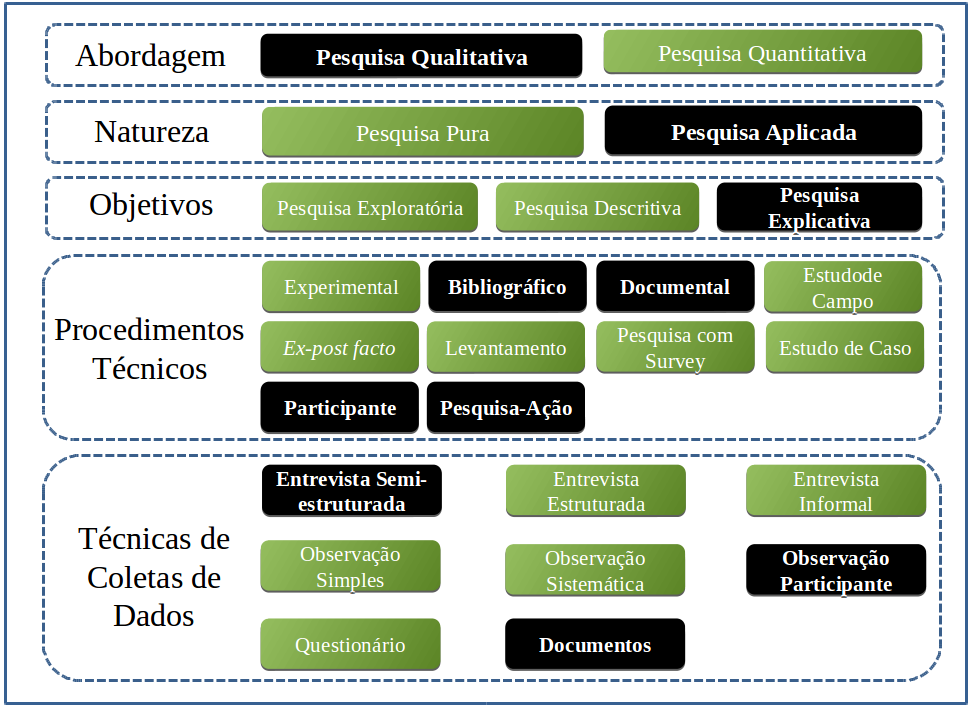
\includegraphics[scale=0.5]{figuras/Metodologia}
	\caption{Seleção da metodologia adotada da pesquisa. Os quadros com fundo preto representam as opções adotadas no presente trabalho.}
	\label{metodologia_adotada}
\end{figure}

Nas subseções seguintes serão detalhados a pesquisa-ação, a pesquisa participante e a entrevista semi-estruturada, que constituem a base metodológica do presente trabalho.

\subsection{Pesquisa-Ação}

Com o grande uso e aumento da sua amplitude e aplicação, a pesquisa-ação tornou-se atualmente um termo aplicado de "forma vaga" a qualquer tipo de tentativa de melhora ou de investigação da prática. A pesquisa-ação ainda pode ser definida como um termo genérico para qualquer processo que siga um ciclo no qual se aprimora a prática pela oscilação sistemática entre agir no campo da prática e investigar a respeito dela \cite{tripp2005pesquisa}.

Para \citeonline{thiollent2009pesquisa} no decorrer da pesquisa-ação ocorre um efeito de aprendizagem, por vezes concebido como conscientização. A pesquisa alimenta a ação e vice-versa, sendo que a aprendizagem é difusa ao longo do processo.

Essa metodologia é caracterizada como um método flexível, qualificada pelo constante ciclo das fases. Assim, o processo de execução, geralmente, não é apresentado em ordem cronológica e sim na forma de um conjunto de ações que, embora não ordenadas no tempo, podem ser consideradas como etapas da pesquisa-ação \cite{gil2002,thiollent2011metodologia}.

É necessário planejar, implementar, descrever e avaliar uma mudança para melhoria de sua prática, aprendendo mais, no decorrer do processo, tanto a respeito da prática quanto da própria investigação \cite{tripp2005pesquisa}. Estas ações estão inseridas nas quatro grandes fases descritas por \citeonline{thiollent2009pesquisa} para a pesquisa-ação: Fase exploratória, na qual os atores da pesquisa começam a detectar problemas a serem combatidos; Fase de pesquisa, na qual coletam-se dados com diversos instrumentos e a pesquisa é discutida pelos membros; Fase de ação, na qual definem-se objetivos, apresentam-se propostas e resultados; e por fim, a fase de avaliação, na qual se obtém conhecimento produzido pela pesquisa e análise dos resultados alcançados.

Segundo \citeonline{thiollent2009pesquisa}, o processo de pesquisa-ação não existe de forma padronizada, pois, dependendo da situação social ou do quadro organizacional em que se aplica, os procedimentos e a ordenação das etapas podem variar. O autor também destaca que as três primeiras fases podem ocorrer simultaneamente.

\begin{comment}
Baseado nessas informações sobre o processo de pesquisa-ação, além das quatro fases básicas previstas, vamos adotar mais uma fase adicional, a fase de coleta de dados, e seguir uma adaptação das fases do processo conforme estabelecido por \citeonline{coughlan2002action}. Dessa forma iremos neste trabalho adotar o processo de pesquisa ação exibido na figura 2, para a condução do procedimento.


Baseado nessas informações sobre o processo de pesquisa-ação, das quatro fases básicas previstas, foram adotadas somente três, ficando excluída a fase de avaliação, por questões de viabilidade do escopo do trabalho (avaliação da efetividade da ação será um trabalho futuro). Essas fases adotadas foram utilizadas na adaptação das fases do processo estabelecido por \citeonline{coughlan2002action}, e o processo de pesquisa-ação adotado neste trabalho é ilustrado na Figura \ref{figura_pesquisa_acao}, onde a cor amarela indica que a fase está fora do escopo do trabalho.

\begin{figure}[!htb]
	\centering
	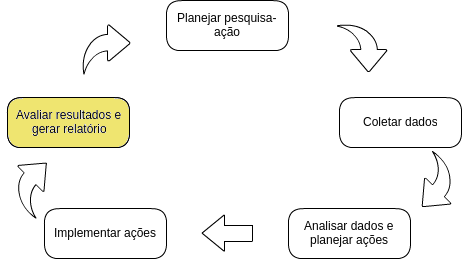
\includegraphics[scale=0.6]{figuras/estruturacao_pesquisa_acao_2}
	\caption{Estruturação para pesquisa-ação. Fonte: \cite{coughlan2002action}, adaptado}
	\label{figura_pesquisa_acao}
\end{figure}

\end{comment}

\newpage
%\vspace{valor}

\subsection{Pesquisa Participante}
A pesquisa participante é caracterizada pela interação entre os pesquisadores e as pessoas envolvidas nas situações investigadas, possui uma diferença sutil da pesquisa-ação, pois possui um propósito de emancipação das pessoas ou das comunidades que a realizam, ou seja, ela é escolhida por quem de antemão se propõe a lutar junto a comunidades excluídas \cite{gilNovaes}.

A Pesquisa Participante se desenvolve a partir da interação entre pesquisadores e membros das situações investigadas. Em uma pesquisa tradicional a população pesquisada é considerada passiva. Enquanto simples reservatório de informações, incapaz de analisar a sua própria situação e de procurar soluções para seus problemas. Nesse  caso, a pesquisa fica exclusivamente a cargo de "especialistas" (sociólogos, economistas etc.), pois somente estes possuiriam a capacidade de formular os problemas e de encontrar formas de os resolver. Desse modo, os resultados da pesquisa ficam reservados aos pesquisadores, e a  população não é levada a conhecer tais resultados e menos ainda a discutí-los \cite{leBoterf}.

Não existe um modelo único de "pesquisa participante", pois trata-se, na verdade, de adaptar em cada caso o processo às condições particulares de cada situação concreta (os recursos, as limitações, o contexto sociopolítico, os objetivos perseguidos etc.) \cite{leBoterf}.

Suas características essenciais são:

\begin{itemize}
	\item a realização concomitante da investigação e da ação;
	\item a participação conjunta de pesquisadores e de pesquisados;
	\item a proposta político-pedagógica em favor dos oprimidos (opção ideológica);
	\item o objetivo de mudança ou transformação social;
\end{itemize}

Esta técnica permite detectar conflitos, tensões e a identificação de viabilidade das mudanças. Assim, duas competências são imprescindíveis para o pesquisador:

\begin{itemize}
	\item Ter postura política voltada às transformações sociais; 
	\item Estar capacitado a promovê-la, como observador e como analista.
\end{itemize}

Segundo \cite{costaSantosTrevisan} a observação participante pressupõe cinco fases:

\begin{itemize}
	\item aproximação do grupo;
	\item processo de inserção;
	\item observação;
	\item análise crítica dos dados colhidos;
	\item retorno para discussão e avaliação dos resultados;
\end{itemize}

Nesse tipo de pesquisa o grupo tem expectativas com relação a pesquisadores. Muitas dessas expectativas incluem preconceitos e desconfianças. Assim, uma das tarefas do pesquisador é destruir as barreiras que bloqueiam a relação com o grupo \cite{costaSantosTrevisan}.

O pesquisador deve considerar que ele é um elemento que está no grupo, mas não é do grupo. Ele possui um papel que transcende ao grupo. Portanto, é preciso que seja aceito na função que de fato tem, ou seja, um pesquisador interessado em analisar um problema no grupo \cite{costaSantosTrevisan}.

\subsection{Pesquisa-Ação Participante}

Várias são as técnicas da pesquisa convencional que são utilizadas na Pesquisa Ação e Participante. Assim é que ambas distinguem uma fase de conhecimento da área, no momento que antecede o entrosamento dos pesquisadores com a população pesquisada (ou “interessada”) onde aquelas lançam mão de estudos existentes, de dados secundários de várias espécies no sentido de se conscientizarem da realidade que se apresenta. Lançam mão, das técnicas da observação participante e da entrevista na coleta de dados primários \cite{costaSantosTrevisan}.

Quanto a diferenciação da pesquisa-ação e pesquisa participante, segundo \citeonline{thiollent2009pesquisa} toda pesquisa-ação é do tipo participativa: a participação das pessoas implicadas nos problemas investigados é absolutamente necessária. No entanto, tudo que é chamado de pesquisa participante não é pesquisa-ação. Isso porque pesquisa participante é em alguns casos um tipo de pesquisa baseado numa metodologia de observação participante na qual os pesquisadores estabelecem relações comunicativas com pessoas ou grupos da situação investigada com o intuito de serem melhor aceitos. Nesse caso, a participação é sobretudo participação dos pesquisadores e consiste em aparente identificação com os valores e os comportamentos que são necessários para a sua aceitação pelo grupo considerado.

Dado a proximidade das duas pesquisas e como as suas diferenças tem como base que a pesquisa participante tem o propósito de emancipação do pesquisador, fazendo parte e sendo aceito pela comunidade em que atua, podendo assim ter a liberdade de decisão sobre as ações referente a comunidade. Pode-se então aliar o procedimento das fases da pesquisa-ação com as fases da pesquisa participante seguindo o conceito dos dois procedimentos.

A partir dos conceitos das duas pesquisas, foi tomado para o trabalho a integração dos conceitos destes dois procedimentos juntamente com suas fases adaptadas ao contexto do trabalho, pois uma vez que os dois procedimentos permitem adaptações de suas fases ao contexto onde se está aplicando, foi elaborado e adaptado as fases para o contexto analisado. 

\begin{comment}
Tomando então como base a Figura \ref{figura_pesquisa_acao}, na fase "analisar dados e planejar ações" da pesquisa-ação elaborou-se o seguinte ciclo para pesquisa participante conforme a Figura :
\end{comment}

O ciclo de construção da solução foi planejado com base na pesquisa participante, conforme a Figura \ref{figura_pesquisa_participante}. \clearpage

\begin{figure}[!htb]
	\centering
	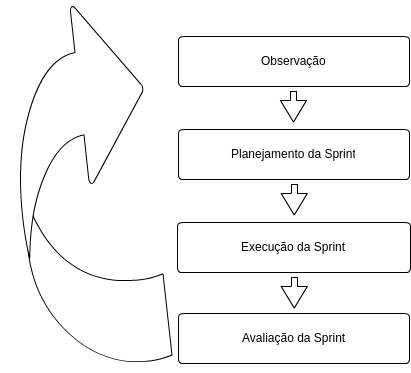
\includegraphics[scale=0.6]{figuras/Fases_pesquisa_participante}
	\caption{Estruturação para pesquisa participante. Fonte: \cite{costaSantosTrevisan}, adaptado}
	\label{figura_pesquisa_participante}
\end{figure}

 Este ciclo contempla as fases da pesquisa participante "aproximação do grupo" e "processo de inserção", pois um dos pesquisadores está inserido no local pesquisado, e o outro já fez parte do mesmo. Para as fases "observação", "análise crítica dos dados colhidos" e "retorno para discussão e avaliação dos resultados", foi elaborado de acordo com a Figura \ref{figura_pesquisa_participante} as fases "observação", "planejamento da sprint", "executar a sprint" e "avaliação da sprint" que irão ser percorridas em ciclos iterativos, sendo n iterações a depender do andamento da implementação da solução ou sistema e de acordo com cada observação realizada em cada iteração.

Cada fase adaptada da pesquisa participante temos o seguinte paralelo e objetivo:

\begin{itemize}
	\item Observação: Será relizada a verificação dos dados obtidos e das necessidades observadas enquanto participante do ambiente pesquisado, no caso o órgão inserido.
	\item Planejamento da Sprint: Faz-se uma equivalência com a fase de análise crítica dos dados colhidos da pesquisa participante, onde nesse caso é realizada uma análise dos dados obtidos e das necessidades observadas fazendo adequações necessárias e realizando o planejamento da sprint com os objetos a serem implementados.
	\item Execução da Sprint: Nessa fase são implementados os objetos planejados na sprint.
	\item Avaliação da Sprint: Essa fase é equivalente a fase de retorno para a discussão e avaliação dos resultados da pesquisa participante, onde será avaliado e discutido os resultados da sprint, podendo caso necessite, realizar mudanças no escopo que foi planejado como alterar, incluir ou retirar dos dados obtidos os objetos a serem implementados sempre objetivando o que é melhor para o órgão, uma vez que o pesquisador é envolvido e faz parte do mesmo.
\end{itemize}



\subsection{Entrevista Semi-Estruturada}

\begin{comment}
------------
--Esse cai fora!!!--
O estudo de caso consiste no estudo profundo e exaustivo de um ou mais objetos, de forma a obter conhecimento amplo e detalhado sobre o mesmo. Segundo \citeonline{yin2001estudo} o estudo de caso é a abordagem mais adequada para a investigação de um fenômeno em seu contexto real, onde os limites entre este fenômeno e o seu contexto não são claramente percebidos. Os propósitos do estudo de caso são \cite{gil2002}:

\begin{itemize}
	\item Explorar situações de contextos reais onde os limites não estão claramente definidos.
	\item Preservar o caráter unitário do objeto.
	\item Descrever a situação do contexto do qual esta sendo feita a investigação.
	\item Desenvolver teorias e formular hipóteses.
	\item Determinar as causas de um determinado fenômeno onde a complexidade não permite o uso de levantamentos e experimentos.
\end{itemize}
--Esse cai fora!!!--
--------------
\end{comment}

Existem diversos métodos de coleta de dados para suportar os propósitos de um procedimento técnico, e um dos métodos comumente usados na engenharia de software é a entrevista \cite{caseStudySE}. A entrevista é caracterizada como um método de coleta de dados onde o pesquisador está em contato direto com os entrevistados e como um método de coleta de dados em tempo real \cite{caseStudySE}. O diálogo entre o entrevistador e o entrevistado é guiado por um conjunto de perguntas, que podem ser classificadas como abertas ou fechadas \cite{caseStudySE}. As perguntas abertas permitem uma maior gama de respostas e relatos de problemas por parte do entrevistado. Já as perguntas fechadas oferecem alternativas mais limitadas, se comparadas as perguntas abertas.

Segundo \citeonline{caseStudySE}, a entrevista pode ser classificada em três categorias diferentes:
\begin{enumerate}
	\item \textbf{Não-estruturada}: As perguntas são formuladas de forma aberta e de acordo com os interesses do pesquisador. A conversa durante a entrevista irá se desenvolver de acordo com os interesses do entrevistado e do entrevistador.
	\item \textbf{Semi-estruturada}: As questões planejadas não são necessariamente perguntadas na ordem em que estão listadas, tendo o desenvolvimento da conversa influência direta na ordem em que as perguntas são feitas ao entrevistado. Além disso, esse tipo de pesquisa permite o improvisamento e a exploração de problemas levantados durante a conversa. É comum em estudos de caso em engenharia de software.
	\item \textbf{Completamente estruturada}: Todas as perguntas são detalhadamente planejadas de antemão e são feitas exatamente na ordem em que estão listadas. Esse tipo de entrevista se assemelha a \textit{surveys} baseados em questionários, pois se trata de perguntas fechadas.
\end{enumerate}

Uma vez que os dados são coletados, o foco se volta para a análise e interpretação dos mesmos. O objetivo é derivar conclusões dos dados, buscando a compreensão e a formação de padrões em cima dos mesmos, por meio de uma cadeia de evidência. Uma cadeia de evidência significa que o leitor pode chegar aos mesmos resultados e conclusões em cima dos dados coletados \cite{caseStudySE}. A análise e interpretação dos dados pode ser dividida nos seguintes procedimentos \cite{caseStudySE}:

\begin{enumerate}
	\item Os dados são codificados de forma que a cada pedaço do texto, que pode ser uma linha ou um parágrafo por exemplo, é atribuído um código que pode representar um certo tema, uma área, uma construção e assim por diante. Observa-se que um pedaço de texto pode possuir mais de um código e um código pode estar associado a mais de um pedaço de texto.
	\item Identificar um conjunto de hipóteses em cima dos dados codificados.
	\item Formar um conjunto de generalizações/conclusões.
	\item Relatar os resultados.
\end{enumerate}

\begin{comment}
\subsection{Metodologia Adotada}
--essa subseção irá sumir, pois não tem mais sentido falar da metodologia adotada, sendo que na parte da metodologia já está se explicando e informando a metodologia que se irá adotar no trabalho--

A metodologia adotada para este trabalho foi o estudo de caso, devido a necessidade de realizar um diagnóstico da situação atual para a construção da solução de apoio, e o método utilizado no estudo de caso foi a entrevista, por ser um método bastante comum neste tipo de metodologia e permitir um contato direto com os entrevistados.

A entrevista elaborada pode ser classificada como semiestruturada. No planejamento da entrevista, algumas categorias de perguntas relacionadas ao ciclo de vida do software e ao contexto do desenvolvedor foram elaboradas, de forma a auxiliar na formulação das perguntas.
\end{comment}

\begin{comment}
%TODO: Unificar pesquisa participante junto com a descrição na parte teórica da metodologia, onde é descrito o estudo de caso.
\subsection{Pesquisa Participante}

--Pesquisa participante--
%TODO: Unificar dentro da metodologia também, ou mover esta sub-seção para antes da sub-seção "Metodologia Adotada".

--Essa parte irá sumir, pois ela virou uma técnica adotada chamada observação participante e já foi abordada na metodologia--
\end{comment}
\subsection{Fases da Pesquisa}

A partir da metodologia, foram definidas as fases e etapas do trabalho, sendo que as fases foram:

\begin{itemize}
	\item Definição do trabalho,
	\item Pesquisa bibliográfica,
	\item Pesquisa-ação participante e documental,
	\item Coleta de dados
\end{itemize}

Na Figura \ref{plano_metodologico} pode-se observar o plano metodológico adotado para este trabalho e em seguida
uma descrição de cada uma das fases.

\begin{figure}[!htb]
	\centering
	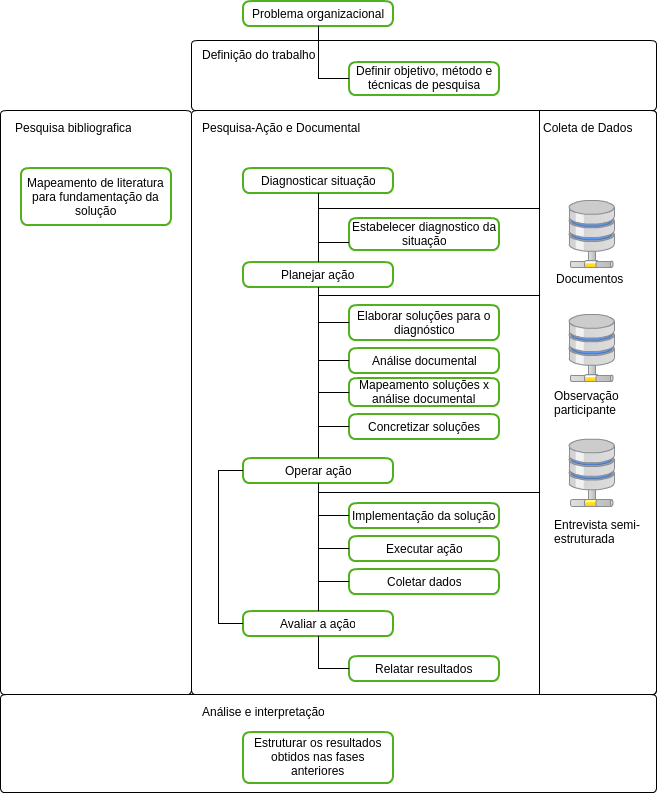
\includegraphics[scale=0.6]{figuras/Plano_metodologico}
	\caption{Plano metodológico adotado. Fonte: autores}
	\label{plano_metodologico}
\end{figure}

\newpage

\textit{Definição do Trabalho}

Esta etapa compreende o estabelecimento do trabalho, com base no problema
organizacional levantado em alto nível. Nesta etapa foram definidos o objetivo a ser atingido, a pergunta de pesquisa, a seleção metodológica e as fases da pesquisa.

\textit{Pesquisa Bibliográfica}

As pesquisas bibliográficas foram realizadas ao longo de toda a pesquisa-ação participante. Esta fase oferece apoio, principalmente, para o planejamento da ação, sendo que é nela onde ocorre o mapeamento da literatura para a construção do referencial teórico e definição da ação a ser aplicada.

\textit{Pesquisa-Ação Participante e Documental}

Esta fase é a base do trabalho, onde foram realizadas as etapas definidas do processo de pesquisa-ação e participante, dentro do órgão público de estudo. A fase buscou entender os problemas ocorridos durante a aplicação do desenvolvimento de sistemas descentralizados, através da experiência de vivência no órgão e pelos documentos inerentes ao processo, afim de encontrar uma solução de apoio. Uma vez que a solução de apoio foi encontrada, ela foi implementada.

\textit{Coletas de dados}

Esta fase inclui a realização de entrevistas e análise dos documentos e experiências do órgão público de estudo referentes ao desenvolvimento descentralizado.

\begin{comment}
\textit{Análise e Interpretação}

Nesta fase os resultados obtidos nas fases anteriores foram analisados.
\end{comment}
\section{\textit{Organização do Trabalho}}

\begin{comment}
\textbf{-- TODO: registrar como está organizado--
--Falar que a partir do capítulo 2 ao 3 (vai entrar mais) trata-se do referencial teórico--}
\end{comment}

Este trabalho está organizado em seis capítulos. Neste capítulo 1, são
apresentados: o contexto do trabalho, o problema com a questão da pesquisa, os
objetivos, a justificativa e a metodologia de pesquisa adotada.

Os capítulos 2 e 3 apresentam o referencial que embasa este trabalho. O referencial teórico é o meio em que o autor do trabalho demonstra o seu conhecimento sobre uma determinada área de estudo (teorias, vocabulários, variáveis chave, fenômenos, métodos e história) \cite{randolph2009}.

O capítulo 4 materiais e métodos traz uma caracterização do órgão de estudo, a descrição das etapas usadas na elaboração do modelo da solução (execução das entrevistas e análise documental no órgão), e o relato do processo de implementação da solução, de acordo com a metodologia definida.

No capítulo 5 é mostrado os resultados obtidos no trabalho, onde apresentam-se as atividades e guias resultantes e complementares do diagnóstico obtido, o sistema final construído e a avaliação da conformidade do sistema com o diagnóstico obtido.

No capítulo 6 é apresentado a conclusão e os trabalhos futuros.

Encontra-se ainda o apêndice do trabalho, onde são apresentadas as perguntas das entrevistas que foram elaboradas no "Apêndice A" e as respostas das entrevistas que foram aplicadas no "Apêndice B".

\chapter[EUD e Desenvolvimento descentralizado]{EUD e Desenvolvimento descentralizado}

\section{\textit{Considerações Iniciais}}

Neste capítulo será apresentado um referencial teórico sobre o \textit{End User Development}, sobre o desenvolvimento descentralizado, diferenciando este do \textit{End User Development}, e sobre o APEX, ferramenta adotada no desenvolvimento descentralizado no órgão público de estudo.

\section{\textit{End User Development}}

\textit{End User Development} (Desenvolvimento por usuário final) é um modelo de desenvolvimento de software onde o usuário final é o principal responsável pela construção do software. \citeonline{lieberman2006} define o \textit{End User Development} (EUD) como um conjunto de métodos, técnicas e ferramentas que permite aos usuários de sistemas de software, que agem como desenvolvedores de software não profissionais, em algum ponto, criar, modificar ou estender um artefato de software.

Para que o desenvolvimento seguindo este modelo possa ocorrer é necessário que existam meios para que o usuário final possa desenvolver e adaptar o software, e para tanto a tecnologia envolvida deve diminuir o esforço cognitivo necessário para a construção do software, através da aproximação conceitual entre as ações do mundo real e as do mundo da programação \cite{fischer2004}. Os usuários finais geralmente não possuem habilidades de um profissional da área de software, e também não estão interessados em construir sistemas no mesmo nível que esses profissionais, por isso é necessário que a tecnologia usada no desenvolvimento alinhe a complexidade relacionada a esta atividade com as habilidades do usuário final. A motivação dos usuários finais é algo essencial para o favorecimento deste modelo, e fatores como o empoderamento, a velocidade de desenvolvimento, a flexibilidade e o controle influenciam diretamente na motivação desses usuários.

O principal objetivo do EUD é oferecer meios para que os usuários finais consigam desenvolver e adaptar software \cite{lieberman2006}. Desta maneira, as aplicações preparadas para o EUD devem ser, principalmente, flexíveis, fáceis de se entender, de se usar, e de se ensinar \cite{lieberman2006}. A preocupação com a tecnologia usada neste modelo de desenvolvimento, mais especificamente na parte das linguagens de programação e aplicações de desenvolvimento, é a relação escopo de aplicação versus esforço de aprendizagem. A Figura \ref{aplicacao_custo_aprendizagem} ilustra a relação do escopo de aplicação e do custo de aprendizagem, para diferentes linguagens de programação e aplicações. Linguagens de programação mais tradicionais como C++ e JAVA oferecem a possibilidade de construção de software de uma grande variedade de domínios, porém a um alto custo associado ao esforço de aprendizagem. Outras linguagens possuem um menor esforço de aprendizagem, ao custo de uma limitação no escopo de aplicação. As linguagens ou aplicações de desenvolvimento ideais para o EUD são as que possuem um alto escopo de aplicação e um baixo esforço de aprendizagem \cite{fischer2004}. As que existem atualmente só utilizam uma pequena parte do potencial do EUD, com algumas falhas \cite{paterno2013}.

\begin{figure}[h]
	\centering
		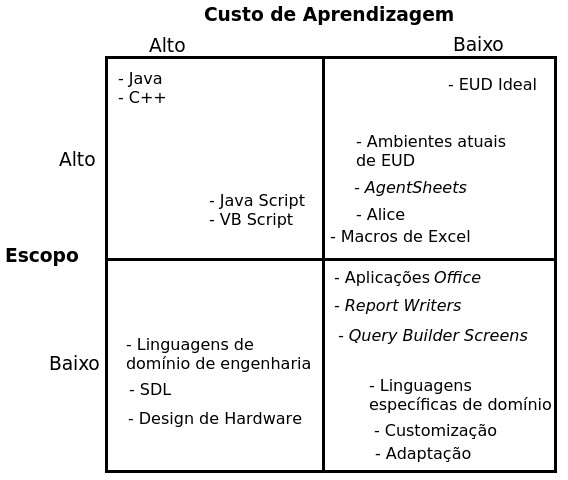
\includegraphics[scale=0.8]{figuras/trade_off_eud_editado}
	\caption{Relação escopo de aplicação e custo de aprendizagem. Adaptado de: \cite{fischer2004}}
	\label{aplicacao_custo_aprendizagem}
\end{figure}
\pagebreak

\citeonline{lieberman2006} classifica as atividades do usuário final em dois tipos:

\begin{enumerate}
\item \textbf{Parametrização ou Customização:} São atividades que permitem o usuário escolher comportamentos, apresentações e mecanismos  alternativos, que já existem dentro de uma aplicação.

\item \textbf{Criação e modificação de programas:} São atividades que implicam na criação ou modificação de artefatos de software. Macros e linguagens de \textit{script} são exemplos deste tipo de atividade.
\end{enumerate}

\subsection{End User Programming}

Programação do usuário final (EUP) é definida como "programação para atingir o resultado de um programa, em vez do próprio programa" \cite{ko2011state}. Em EUP, o objetivo do desenvolvedor é realmente usar o programa, isso contrasta com a programação profissional, onde o objetivo é criar um programa ou sistema para que outras pessoas possam usar, na maioria das vezes em troca de valores que precificam o sistema, ou seja, na venda de seu sistema.

Os programas criados através do EUP podem ser extensões das aplicações existentes, ou podem ser novas aplicações que rodam separadamente dos que já existem. Os usuários finais podem executar EUP através de uma vasta gama de estilos de interação \cite{nardi1993small}.

\subsection{End User Software Engineering}

Outro conceito relacionado ao EUD é a engenharia de software do usuário final (EUSE). EUSE é relativamente um novo subconjunto de EUD que começou há cerca de uma década atrás. Sua ênfase está na qualidade do software aos usuários finais para os mesmos possam cria-lo, modifica-lo ou estende-lo; dessa forma a sua investigação centra-se sobre os métodos, técnicas e ferramentas que promovam a qualidade de tal software. Esta área tem surgido por causa da ampla evidência de que os programas criados por usuários finais são desenvolvidos com erros no final podem custar caro a uma organização \cite{panko1998we,burnett2010technology,ko2011state}.

A engenharia de software do usuário final (EUSE) é definida como "a programação do usuário final envolvendo atividades sistemáticas e disciplinadas que tratam de questões de qualidade de software" \cite{ko2011state}.

A atenção à qualidade é importante para o EUP porque um software mal escrito pode causar perda de dados, falhas de segurança, perda financeira, ou até mesmo danos físicos.

As qualidades de software relevantes para EUSE são os mesmos que os de interesse para desenvolvedores profissionais que vendem seus produtos. Essas qualidades incluem confiabilidade, desempenho, facilidade de manutenção, reutilização, privacidade e segurança. Algumas qualidades, tais como manutenção e reutilização, só se tornam visíveis depois que um programa foi escrito e está em funcionamento há algum tempo. Assim, EUSE combina com o objetivo do EUP, permitindo que os usuários finais criem software, com a preocupação de qualidade desse software em toda a sua amplitude de um ciclo de vida. Este ciclo de vida inclui requisitos de criação do sistema, verificação, depuração, e a reutilização de código \cite{ko2011state}.

\subsection{Requisitos e Projeto}

Requisitos descrevem o que um programa deve fazer, e o projeto refere-se à determinação de como um programa deve fazê-lo. Por exemplo, um requisito pode ser um programa que deva ser capaz de ordenar uma lista de endereços de usuários; e seu \textit{design} ou projeto poderia ter detalhes do algoritmo de ordenação a ser usado.

Exemplos de requisitos (metas) em EUD incluem personalizar a maneira que um aplicativo ou computador se comporta, automatizando tarefas demoradas, realizando cálculos que são difíceis de fazer com precisão, ou comunicar informações \cite{ko2011state,blackwell2003notational,rosson2005minimalist}.

Obter estes requisitos de forma correta é um aspecto crítico da perspectiva de EUSE, por causa de sua ênfase na qualidade. Espera-se que os desenvolvedores profissionais investiguem, documentem e refinam os requisitos antes de começarem a desenhar ou codificar uma aplicação. Por exemplo, eles podem tentar identificar inconsistências nos requisitos através da aplicação de uma das várias técnicas meticulosas, por exemplo, revisão das partes interessadas ou modelagem formal. Em contraposição, os usuários finais muitas vezes já tem uma idéia sobre as exigências necessárias para a aplicação, e descartam qualquer trabalho extra para alcançar esses requisitos e documentá-los.

Segundo \citeonline{Faily2008}, durante a preparação de casos de uso, os usuários possuem problemas com o nível de conhecimento em engenharia de software, eles acreditam que estão, implicitamente, assumindo o processo. Na sequência da elaboração inicial de casos de uso para diferentes cenários de geração, os usuários relatam problemas com a compreensão do significado das partes constituintes ao usar modelo de caso de uso.

Assim, por vezes, os usuários finais não sabem os requisitos com antecedência e não visualizam um \textit{design}, eles esperaram que esses assuntos sejam esclarecidos durante a evolução da implementação do programa \cite{costabile2006supporting,fischer2006meta,morch2000tailoring}. Desenvolvedores profissionais, muitas vezes, também não conhecem os requisitos com antecedência, mas eles são capazes de tomar medidas para lidar com essa situação, como por exemplo, empregando um método iterativo que obtém os requisitos através do uso de protótipos afim de evoluí-los, ao invés de omiti-los completamente e seguir em frente. No entrando, os desenvolvedores EUD podem ir diretamente para codificação sem tomar o tempo necessário para documentar as suas necessidades ou procurar inconsistências \cite{rosson2013end}.

Uma abordagem para os desenvolvedores EUD é a busca de uma revisão junto à pares mais experiente. Oa identificar listas curtas de melhores práticas e fornecer ferramentas adequadas, os pesquisadores têm tentado fazer essa prática tão eficiente quanto possível, de modo que possa ser aplicado sem abrandar consideravelmente o ciclo de vida do EUD \cite{powell2008management,rosson2013end}. Tal abordagem parece ser bem sucedida em um ambiente organizacional, onde os desenvolvedores EUD tem colegas a quem recorrer e onde a hierarquisa de gestão pode ser usada, se necessário, para impor e fazer cumprir as revisões de projeto.

\subsection{Verificação e Validação}

Verificação e validação abrangem atividades que tentam certificar que um programa faz o que é pressuposto a fazer. O teste é a abordagem mais comum para a verificação e validação. Um dos primeiros trabalhos de apoio à verificação e validação em EUD, foi para ajudar os usuários finais avaliar se os seus programas continham erros, encorajando-os a testar de forma estratégica. Talvez a abordagem de teste do usuário final mais desenvolvida é o \textit{"What You See Is What You Test"} (WYSIWYT) ou o que você vê é o que você testa, que orienta os usuários a testarem sistematicamente \cite{fisher2006integrating}. O WYSIWYT emprega uma estratégia de \textit{Surprise-Explique-Reward}, em que surpreende com bordas coloridas para atrair atenção às áreas que precisem de testes, dando dicas de ferramentas que expliquem o significado das cores aos usuários, e mostrando a potencial recompensa no uso da ferramenta \cite{wilson2003harnessing}.

\subsection{Depuração}

Depois que um erro de programação é detectado, o próximo passo é removê-lo por depuração. Algumas das técnicas de depuração utilizadas por desenvolvedores profissionais foram adaptadas para o uso em ferramentas EUP. Além de inserir declarações que imprimem os valores das variáveis de um programa em execução, os desenvolvedores EUD podem percorrer instruções uma a uma, observando as operações que estão incorretas \cite{leshed2008coscripter}. Afirmações, representam uma outra técnica importante que tem sido adaptada para uso em EUP. Um usuário pode inserir uma instrução condicional no código, e a execução do programa irá chamar a atenção para este ponto se a instrução inserida for avaliada como falsa em tempo de execução \cite{burnett10,koesnandar2008using,scaffidi2008topes}.

Várias outras ferramentas EUP que suportam técnicas de teste, podem alavancar os resultados de teste para facilitar a depuração.

\subsection{Reuso}

Quando o código é escrito, a reutilização pode acelerar a criação de programas posteriores. Apoiar a reutilização de programas de EUD é um desafio, pois os desenvolvedores EUD raramente têm a oportunidade e a formação exigida para projetar programas altamente reutilizáveis. Outro desafio é que os desenvolvedores EUD podem cometer erros ao criar programas e reutilizar estes códigos podem propagar erros nestes programas dentro de uma organização \cite{mackay1990patterns}. Portanto, mesmo que sistemas com repositórios ou servidores de arquivos possam tornar mais fácil para os desenvolvedores EUD deixar programas ou códigos preparados para reutilização, eles podem tornar extremamente maior a dificuldade por parte de outros desenvolvedores, a avaliação do código desses programas que será reutilizado. Para ajudar a reduzir a dificuldade de reutilização de programas, modelos de programas EUP reutilizáveis estão em desenvolvimento na esperança de ajudar os usuários a procurarem repositórios de programas reutilizáveis relacionados com os seus interesses particulares \cite{scaffidi2010using} (Scaffidi et al 2010). Além disso, um outro trabalho começou a explorar uma forma de ajudar os usuários a extraírem partes reutilizáveis de um programa \cite{oney2009firecrystal}.

\subsection{Oracle Application Express - APEX}

O Oracle Application Express (APEX) é uma ferramenta que permite criar, personalizar e implementar aplicações em cima do banco de dados Oracle, usando apenas um navegador de internet. O APEX é um ambiente de desenvolvimento gratuito para construir aplicações usando SQL e PL/SQL e que apresenta uma plataforma extensível, executada dentro do banco de dados Oracle \cite{oracleApex}. O APEX tem como objetivo diminuir a complexidade de desenvolvimento das aplicações, ao fornecer um ambiente interativo e de fácil manuseio para construir e executar as aplicações, garantindo que tanto desenvolvedores não profissionais quanto desenvolvedores experientes desenvolvam com agilidade. As funcionalidades da aplicação são criadas de forma fácil e rápida. As vantagens do APEX incluem \cite{oracleApex}:
\begin{itemize}
	\item Velocidade de entrega;
	\item Maior controle e precisão no desenvolvimento;
	\item Facilidade para a criação de protótipos;
	\item Facilidade de implantação;
	\item Aplicação acessada via navegador (URL);
	\item Grande quantidade de usuários (desenvolvedores) ativos;
\end{itemize}

Além disso, o ambiente de desenvolvimento integrado é muito intuitivo, o que torna a introdução e a adoção do APEX uma transição fácil para desenvolvedores experientes ou usuários finais.

O APEX usa uma arquitetura simples, onde as páginas são geradas dinamicamente usando metadados armazenados no banco de dados Oracle. Não há geração de código ou compilação de arquivos. Uma vez que ele foi instalado e configurado, a URL será a via de acesso ao ambiente de desenvolvimento e às aplicações, tanto para os desenvolvedores quanto para os usuários finais. As alterações feitas durante o desenvolvimento são salvas diretamente nas tabelas de metadados, que contém as definições das aplicações. Após isso o desenvolvedor pode executar a aplicação e revisar as melhorias imediatamente.
Para a implantação e execução do APEX é necessário um servidor web, um servidor de aplicação, um servidor APEX \textit{listener} e um servidor de banco de dados Oracle, conforme a Figura \ref{arquitetura_apex}.
\clearpage

\begin{figure}[!htb]
	\centering
	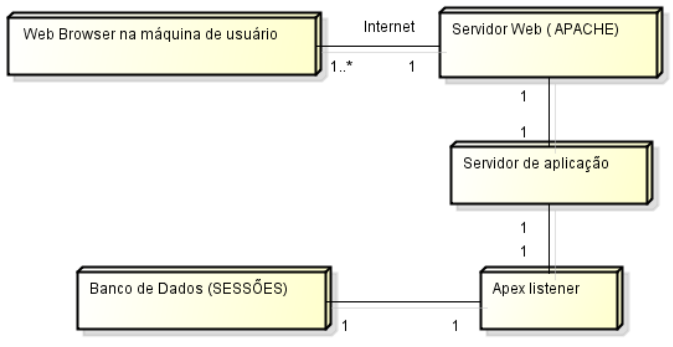
\includegraphics[scale=0.6]{figuras/arquitetura_apex}
	\caption{Arquitetura do APEX. Fonte: \cite{ferreira2015}.}
	\label{arquitetura_apex}
\end{figure}

O fluxo de dados na arquitetura do APEX, é composto dos seguintes passos \cite{ferreira2015}:
\begin{enumerate}
	\item Uma requisição HTTP é enviada, pelo navegador, quando o usuário acessa uma página da aplicação;
	\item O servidor web recebe a requisição e identifica que é uma requisição do APEX, redirecionando a requisição ao servidor de aplicação correto;
	\item O servidor de aplicação organiza os pedidos (filtros, \textit{cache}, \textit{timeouts}, filas, etc) e transfere para o APEX \textit{listener}.
	\item O APEX \textit{listener} recebe o pedido e executa os comandos Java que irão ler os dados do banco e/ou executar códigos PL/SQL. O APEX \textit{listener} interage com sessões de banco, onde os dados são buscados.
	\item Faz-se o caminho inverso com os dados coletados, os PL/SQLs executados e os códigos HTML, \textit{Javascript}, CSS, \textit{Ajax} e \textit{jQuery} gerados, que são devolvidos ao navegador que então mostra a tela da aplicação ao usuário.
\end{enumerate}

\clearpage

\section{Desenvolvimento descentralizado}

 Alguns órgãos da administração pública federal brasileira começam a ter a iniciativa de adotar este modelo. A diferença entre o EUD e o desenvolvimento descentralizado é que no desenvolvimento descentralizado não é necessariamente o usuário final do software quem irá desenvolve-lo \cite{artigoTcuGovTI}. No órgão público de estudo, que foi um dos pioneiros na implantação deste modelo, os projetos que seguem o desenvolvimento descentralizado tem sido desenvolvidos tanto por servidores, quanto por estagiários de cursos da área de TI, que possuem diferentes níveis de conhecimento sobre desenvolvimento de software, e que também não são os usuários finais do software \cite{artigoTcuGovTI}. O desenvolvedor, se for um estagiário, é alocado na área de negócio e um analista de TI é designado para dar suporte técnico, de forma a tentar garantir que o software sendo desenvolvido siga os padrões estabelecidos e garantidos pela TI corporativa \cite{artigoTcuGovTI}.
Dentre as possíveis motivações que tem levado a adoção deste modelo em alguns órgãos da administração pública federal, destacam-se \cite{slideTCU}:

\begin{itemize}
\item Desconhecimento das iniciativas de informatização;
\item Falta de alinhamento estratégico das iniciativas;
\item Duplicidade de esforços das unidades de negócio;
\item Diversidade de ferramentas de desenvolvimento;
\item Elevado risco de descontinuidade;
\item Comprometimento da segurança da informação;
\end{itemize}

Este modelo de desenvolvimento no órgão público de estudo é viabilizado pelo uso da ferramenta Oracle APEX, que permite o desenvolvimento de aplicações seguindo a lógica do EUD.
\clearpage

\chapter[Materiais e Métodos]{Materiais e Métodos}

\section{\textit{Considerações Iniciais}}


Este capítulo trata dos procedimentos executados para se atingir o objetivo de propor a solução de apoio ao desenvolvedor EUD. Inicialmente foi realizada uma caracterização do órgão público alvo do trabalho. Em seguida são apresentadas as etapas utilizadas para a avaliação das entrevistas e dos documentos do órgão (processo de desenvolvimento descentralizado e \textit{Wiki}), que serviram de base para a elaboração do modelo da solução. Por fim é apresentado o relato dos procedimentos realizados para a construção da solução.

\section{Caracterização do Órgão}

O presente trabalho está inserido no contexto do órgão público de estudo, o qual possui duas formas distintas de desenvolvimento de software: uma forma centralizada, que é um método tradicional de desenvolvimento de software (desenvolvimento realizado na área da TI e por profissionais de TI), e uma forma descentralizada, que é um modo menos tradicional de desenvolvimento (desenvolvimento realizado nas áreas de negócio e por pessoas com menos qualificação técnica e experiência, geralmente estagiários).

O desenvolvimento descentralizado no órgão público de estudo segue a linha do EUD (End User Development) e, devido a isso, a forma de desenvolvimento é bastante flexível, variando conforme o contexto da unidade de negócio e a experiência do desenvolvedor. A ferramenta adotada pelo órgão para viabilizar o desenvolvimento descentralizado foi o Oracle APEX, que é bastante amigável e permite que pessoas com muito pouca experiência em programação possam desenvolver aplicações. Percebendo a variação na forma de desenvolvimento dos sistemas, a unidade coordenadora do desenvolvimento descentralizado propôs:

\begin{itemize}
\item Uma \textit{Wiki} com guias e tutoriais relacionados ao desenvolvimento descentralizado de aplicações, voltados à ferramenta APEX;
\item Um processo de desenvolvimento descentralizado, de forma a padronizar este tipo de desenvolvimento dentro do órgão;
\end{itemize}

A \textit{Wiki} é uma fonte importante de conhecimento ao desenvolvimento descentralizado dentro do órgão, e em alguns casos até ao desenvolvimento corporativo. Já o processo foi elaborado em cima da ferramenta \textit{Eclipse Process Framework}, onde ele é detalhado a nível de atividades, tarefas, papéis, guias, marcos e fases. Por falta de meios legais para a institucionalização do processo, o mesmo foi desativado.

O desenvolvimento descentralizado apresenta um bom relato de satisfação no órgão público de estudo, porém considerando a importância da aplicação de boas práticas e padrões neste contexto, existem oportunidades de melhoria.

\begin{comment}
\section{Definição da Proposta}

Tendo em vista o contexto caracterizado, este trabalho se propõe a elaborar uma solução informatizada que possa apoiar o desenvolvimento descentralizado no Órgão X. Esta solução irá conter um conjunto de atividades, de boas práticas e de funcionalidades que possam contribuir para uma melhoria na qualidade e manutenibilidade das aplicações desenvolvidas. Na primeira etapa do trabalho (TCC 1) será identificado o conjunto de atividades e boas práticas da solução, de forma que estas atividades estejam relacionadas entre si através de um fluxograma, e que as boas práticas estejam contidas dentro das atividades, auxiliando a execução das mesmas. Na segunda etapa (TCC 2), espera-se detalhar as atividades e as boas práticas definidas, informatizar o fluxo de atividades e implementar as funcionalidades que possam auxiliar na execução de algumas das atividades da solução.

Para se atingir o objetivo deste trabalho, realizou-se, inicialmente, um levantamento bibliográfico sobre os tópicos relacionados ao trabalho: \textit{End User Development}, desenvolvimento descentralizado, \textit{SCRUM} e \textit{Kanban}. Em seguida foram realizadas entrevistas com o propósito de diagnosticar a situação do desenvolvimento descentralizado no Órgão X, coletando os problemas, as boas práticas e as sugestões de melhorias, relatados pelos próprios desenvolvedores. Foi realizada uma análise no processo de desenvolvimento descentralizado não implementado, existente no Órgão X, com o intuito de verificar quais atividades e guias existentes poderiam dar um suporte à elaboração das soluções relacionadas ao diagnóstico obtido. Uma análise sobre os conteúdos da \textit{Wiki} da unidade coordenadora do desenvolvimento descentralizado também foi feita, de forma a agregar algumas boas práticas, definidas pela unidade, à solução. A partir do diagnóstico, da análise do processo e da análise da \textit{Wiki} foram definidas as atividades e os guias da solução de apoio. Estas atividades foram então relacionadas através de um fluxograma, representando o sequenciamento das mesmas.

%TODO: Explicar aqui a elaboração da entrevista, já que a entrevista é um "método" da pesquisa participante.

\section{\textit{Pesquisa Participante}}
--Falar como a gente abordou a pesquisa participante--
\end{comment}

\section{Entrevistas Realizadas}
As entrevistas tiveram como objetivo realizar um diagnóstico da situação do desenvolvimento descentralizado no órgão público de estudo, sob o ponto de vista do desenvolvedor que está inserido neste contexto. Esse diagnóstico procurou abordar os aspectos de dificuldades enfrentadas pelos desenvolvedores, de boas práticas realizadas e de sugestões de melhorias. Para que esses aspectos pudessem ser abordados na entrevista, as questões foram agrupadas por categorias, sendo estas, em sua maioria, relacionadas as fases de um ciclo de desenvolvimento de software. Cada categoria possui um objetivo, que representa qual o tipo de informação que se pretende obter. Na Tabela \ref{tabela_01} estão expostas as informações desejadas, através dos objetivos, e suas respectivas categorias. \clearpage

\begin{comment}
O objetivo da entrevista consistiu em obter um diagnóstico da situação atual do desenvolvimento descentralizado no Órgão X, para que servisse de insumo para a elaboração da solução de apoio. Como diagnóstico entendeu-se as boas práticas realizadas, as sugestões de melhoria e os problemas. Portanto, a entrevista elaborada tentou abordar esses pontos, consistindo de 34 perguntas divididas em 9 categorias. A entrevista pode ser visualizada no "Anexo A".
\end{comment}

\begin{table}[!htb]
\centering
\caption{Categorias da entrevista e seus objetivos.}
\begin{tabular}{|l|l|}
\hline
\textbf{Categoria}                                                   & \textbf{Objetivo}                                                                             \                                                                                                                                                                                                                                               \\ \hline
\begin{tabular}[c]{@{}l@{}}Descrição do\\ Desenvolvedor\end{tabular} & 1- Obter informações sobre o perfil dos desenvolvedores.                                                                                                                                                                                                                                                                                     \\ \hline
\begin{tabular}[c]{@{}l@{}}Papel do\\ Desenvolvedor\end{tabular}     & 1- Obter informações sobre o papel do desenvolvedor no órgão.                                                                                                                                                                                                                                                                                \\ \hline
\begin{tabular}[c]{@{}l@{}}Efetividade do\\ Treinamento\end{tabular}       & 1- Obter informações sobre a preparação dos novos desenvolvedores.                                                                                                                                                                                                                                                                           \\ \hline
Requisitos                                                           & \begin{tabular}[c]{@{}l@{}}1- Obter informações sobre como se dá o levantamento de requisitos \\ nos departamentos da instituição.\\ 2- Obter informações de como são armazenados e gerenciados os requisitos \\ do sistema a ser desenvolvido.\\ 3- Obter informações de como são englobados as mudanças de requisitos \\ ao sistema.\end{tabular} \\ \hline
\textit{Design}                                                      & \begin{tabular}[c]{@{}l@{}}1- Obter informações sobre como é realizado a modelagem (arquitetura) \\ do sistema.\end{tabular}                                                                                                                                                                                                                 \\ \hline
Codificação                                                          & \begin{tabular}[c]{@{}l@{}}1- Obter informações sobre a depuração de erros do sistema.\\ 2- Obter informações sobre estilos de codificação.\\ 3- Obter informações sobre o ambiente de codificação.\end{tabular}                                                                                                                             \\ \hline
Teste                                                                & \begin{tabular}[c]{@{}l@{}}1- Obter informações sobre a elaboração dos testes, bem como a forma \\ de realizá-los.\end{tabular}
\\ \hline
Implantação                                                          & 1- Obter informações sobre a migração do sistema para a produção.                                                                                                                                                                                                                                                                        \\ \hline
\end{tabular}
\label{tabela_01}
\end{table}

A categoria "Descrição do Desenvolvedor" serviu unicamente para descrever o perfil dos desenvolvedores entrevistados, portanto ela não foi considerada na análise dos resultados obtidos. A partir dessas categorias, foram elaboradas as perguntas, de forma que elas atendessem os o
bjetivos definidos. O \textit{template} da entrevista pode ser visualizada no "Apêndice A". 

Uma vez que a entrevista foi elaborada, o próximo passo consistiu em aplicá-la. A escolha dos desenvolvedores foi feita de forma aleatória, escolhendo-se 8 desenvolvedores diferentes que estão inseridos no contexto do desenvolvimento descentralizado do órgão público de estudo. Os 8 desenvolvedores foram escolhidos devido a objetivação pela qualidade da análise e não pela quntidade e estão divididos entre 7 estagiários e 1 servidor. A Tabela \ref{tabela_02} contextualiza o perfil dos desenvolvedores entrevistados. Observa-se que alguns desses dados não se aplicam ao desenvolvedor 6, por este ser um servidor. \clearpage

\newcolumntype{M}[1]{>{\centering\arraybackslash}m{#1}}
\begin{table}[!htb]
	\centering
	\caption{Perfil dos desenvolvedores entrevistados}
	\begin{tabular}{|M{2.88cm} | M{2.8cm} | M{2.2cm}| M{2.8cm} | M{2.2cm}|}
		\hline
		\textbf{Desenvolvedor} & \textbf{Unidade} & \textbf{Tempo de estágio} &
		\textbf{Curso} & \textbf{Tempo de Curso} \\ \hline
		Desenvolvedor 1 & SECOM & 1 ano & Análise e Desenvolvimento de Sistemas & 2 semestres \\
		\hline
		Desenvolvedor 2 & SCV & 1 ano & Sistemas de Informação & 8 semestres \\
		\hline
		Desenvolvedor 3 & MTCU & 7 meses & Sistemas de informação & 6 semestres \\
		\hline
		Desenvolvedor 4 & SEADE & 7 meses & Análise e Desenvolvimento de Sistemas & 4 semestres \\
		\hline
		Desenvolvedor 5 & SECOF & 1 ano & Sistemas de Informação & 5 semestres \\
		\hline
		Desenvolvedor 6 & SEPROD & - & - & - \\
		\hline
		Desenvolvedor 7 & DISIC & 1 mês & Engenharia de Software & 6 semestres \\
		\hline
		Desenvolvedor 8 & SEPROD & 6 meses & Engenharia de Redes de Comunicação & 9 semestres \\
		\hline
	\end{tabular}
	\label{tabela_02}
\end{table}

Após a aplicação da entrevista, o foco voltou-se a análise dos dados da mesma. A análise feita consistiu dos seguintes passos (P1, P2, P3, P4 e P5):

\begin{enumerate}
	\item[\textbf{\llap{P}1}] Atribuiu-se um código, derivado dos objetivos de cada categoria de questões, a cada unidade de resposta, que pode ser uma frase ou um conjunto de frases que tratem de um mesmo assunto;
	%\item Atribui-se um código, previamente estabelecido, a uma unidade de resposta, que pode ser uma frase ou um conjunto de frases que tratem de um mesmo assunto.
	\item[\textbf{\llap{P}2}] Agrupou-se as unidades de resposta de acordo com os códigos derivados que receberam;
	%\item Agrupou-se as unidades de resposta de acordo com as categorias de código que receberam.
	\item[\textbf{\llap{P}3}] Com a finalidade de identificar as respostas semelhantes dentro dos grupos de códigos derivados, evitando redundância, rotulou-se as unidades de respostas com o uso de chaves, que representam o sentido específico de uma resposta;
	%\item Dentro de uma categoria de código, rotulou-se as respostas com o uso de chaves, que representam o sentido específico de uma resposta.
	\item[\textbf{\llap{P}4}] Agrupou-se todas as chaves únicas obtidas, de forma a construir um conjunto de elementos que representam as oportunidades de melhoria na visão dos desenvolvedores;
	%\item Agrupou-se todas as chaves únicas obtidas, de forma a construir um conjunto de chaves únicas.
	\item[\textbf{\llap{P}5}] Elaborou-se ações para esses elementos;
\end{enumerate}

A Figura \ref{etapas_analise_respostas} mostra um esquema que exemplifica a execução dos passos definidos para a análise. No passo 1 (P1), observa-se o agrupamento das unidades de resposta pelos códigos derivados. Já no passo 2 (P2), observa-se o agrupamento das respostas por códigos derivados. No passo 3 (P3), observa-se as unidades de respostas, dentro dos grupos de códigos derivados, rotuladas com as chaves. Por fim, no passo 4 observa-se os elementos obtidos que representam as oportunidades de melhoria. O passo 5 (P5) será detalhado mais adiante, já que faz parte dos resultados.

\begin{figure}[h]
%	\centering
\hspace*{-1.5cm}
		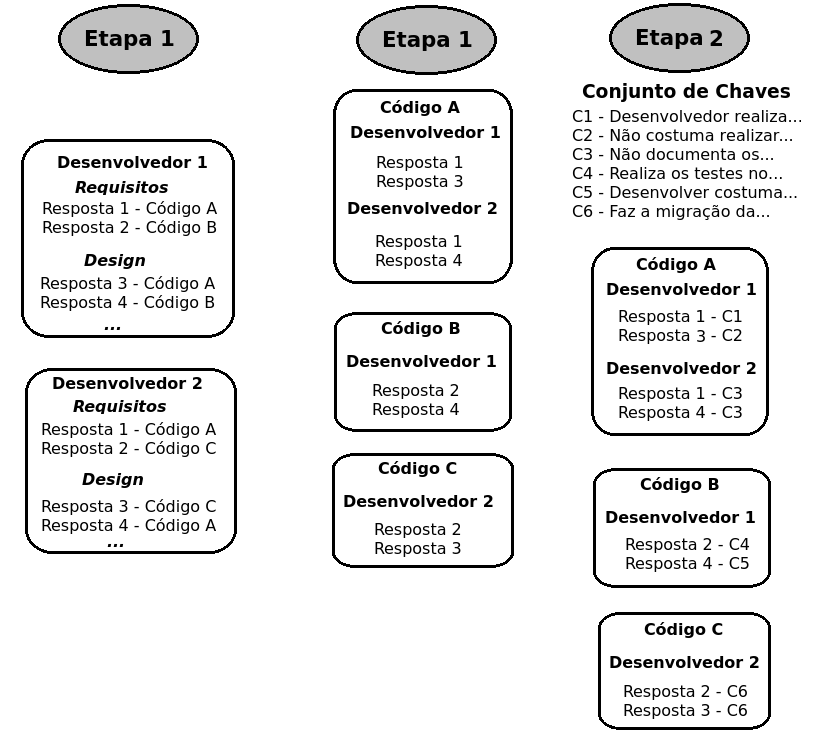
\includegraphics[scale=0.7]{figuras/Esquematico_Analise_2}
	\caption{Etapas realizadas na análise das respostas.}
	\label{etapas_analise_respostas}
\end{figure}

Os códigos foram derivados dos objetivos de cada categoria de perguntas do ciclo de vida. A Tabela \ref{tabela_03} ilustra os códigos derivados de cada objetivo de categoria definido.

\newcolumntype{M}[1]{>{\centering\arraybackslash}m{#1}}
\begin{table}[!htb]
	\centering
	\caption{Códigos elaborados para a análise dos resultados}
	\begin{tabular}{|m{4.8cm} | m{4.8cm} | m{4.8cm}|}
		\hline
		\textbf{Categoria} & \textbf{Objetivo} &
		\textbf{Código Derivado} \\ \hline
		Descrição do desenvolvedor & Obter informações sobre o perfil dos desenvolvedores &
		Perfil do Desenvolvedor \\ \hline
		Papel do desenvolvedor & Obter informações sobre o papel do desenvolvedor no órgão &
		Papel do Desenvolvedor \\ \hline
		Efetividade do Treinamento & Obter informações sobre a preparação dos novos desenvolvedores &
		Preparação \\ \hline
		Requisitos & Obter informações sobre como se dá o levantamento de requisitos nos departamentos da instituição & Elicitação de Requisitos \\ \cline{2-3}
		& Obter informações de como é armazenado e gerenciado os requisitos do sistema a ser desenvolvido &
		Gerenciamento de Requisitos \\ \cline{2-2}
		& Obter informações de como é englobado as mudanças de requisitos ao sistema & \\ \hline
		\textit{Design} & Obter informações sobre como é realizado a modelagem (arquitetura) do sistema &
		Modelagem do sistema \\ \hline
		Codificação & Obter informações sobre a depuração de erros do sistema & Depuração \\ \cline{2-3}
		& Obter informações sobre estilos de codificação & Estilos de codificação \\ \cline{2-3}
		& Obter informações sobre o ambiente de codificação & Ambiente de codificação \\ \hline
		Teste & Obter informações sobre a realização dos testes, bem como a forma de realiza-los &
		Teste \\ \hline
		Implantação & Obter informações sobre a migração, para a produção, do sistema & Implantação \\
		\hline
	\end{tabular}
	\label{tabela_03}
\end{table}

As chaves foram derivadas dos significados das respostas das entrevistas, de forma que se duas ou mais respostas geraram uma mesma chave, devido aos seus significados semelhantes, somente uma única chave foi considerada.

A atribuição de um código e de uma chave foram necessários, pois dentro de um determinado assunto, representado pelo código, ainda poderiam haver respostas semelhantes. Desta forma, garante-se que o conjunto final de chaves conterá somente chaves únicas, ou seja, respostas únicas, eliminando a redundância no diagnóstico.
\clearpage

\section{Processo de Desenvolvimento Descentralizado}

De acordo com o chefe da unidade coordenadora do desenvolvimento descentralizado, houve uma tentativa de implantação de um processo para o desenvolvimento descentralizado já foi realizada pelo órgão público de estudo, evidenciando a necessidade de um processo ou guia para o desenvolvimento descentralizado. O processo, chamado de Processo de Desenvolvimento Descentralizado do órgão público de estudo, teve a sua finalização concluída no ano de 2012, e foi elaborado pela Secretaria de Tecnologia da Informação do órgão. Apesar de o processo ter sido desenvolvido, segundo o chefe da unidade coordenadora do desenvolvimento descentralizado, ele não chegou a ser efetivamente implantado devido a questões normativas do próprio órgão.

O processo, elaborado na ferramenta \textit{Eclipse Process Framework}, que é voltada à construção de processos, consiste de 6 fases bem definidas: Estudo Preliminar de Projeto, Elicitação de Requisitos, Projeto de Banco de Dados, Construção, Homologação e Implantação. Cada uma dessas fases são divididas em atividades e tarefas, que por sua vez são apoiadas por um conjunto de guias e modelos. Os objetivos de cada fase estão listados abaixo, e o ciclo de vida do processo, em termos de fases, é exibido na Figura \ref{ciclo_vida_pdesc}.

\begin{figure}[h]
	\centering
		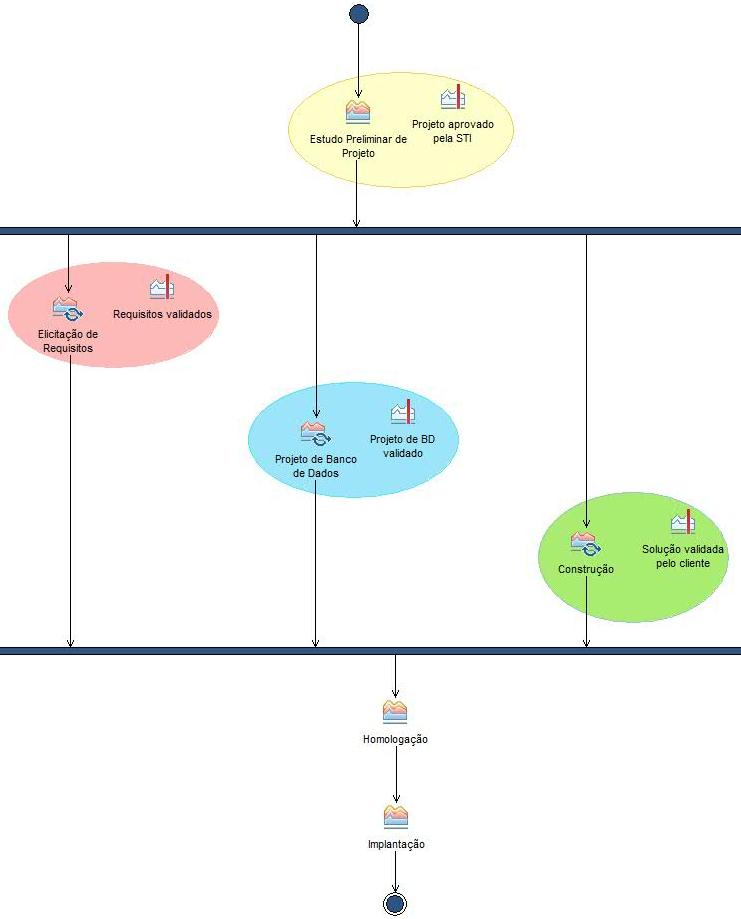
\includegraphics[scale=0.8]{figuras/PDESC}
	\caption{Ciclo de vida do processo de desenvolvimento descentralizado.}
	\label{ciclo_vida_pdesc}
\end{figure}

\begin{enumerate}
	\item \textbf{Estudo Preliminar de Projeto:} Fase destinada à análise da proposta de solução e, caso a proposta seja aprovada, à preparação de recursos.
	\item \textbf{Elicitação de Requisitos:} Fase destinada à elicitação de requisitos e à definição da arquitetura da solução.
	\item \textbf{Projeto de Banco de Dados:} Fase destinada à construção do Modelo de Dados Lógico e do Modelo de Dados Físico da solução.
	\item \textbf{Construção:} Fase destinada à construção da solução.
	\item \textbf{Homologação:} Fase destinada à realização dos testes da solução, à capacitação dos usuários e à divulgação da solução.
	\item \textbf{Implantação:} Fase destinada à implantação da solução.
\end{enumerate}
\clearpage

Foram selecionados para a construção da solução de apoio, os componentes de processo (atividades, tarefas, guias e modelos) que possuem uma relação com os problemas, as sugestões e as boas práticas relatados no diagnóstico, e alguns que não estão relacionados diretamente com o diagnóstico, mas que se julgou interessante para complementar a solução.

\section{\textit{Wiki} do Desenvolvimento Descentralizado}

O órgão público de estudo utiliza um sistema de \textit{Wiki} como uma das formas de compartilhamento de informação entre o público interno do órgão, de forma que esse público possa usufruir e contribuir com as informações publicadas. A unidade coordenadora do desenvolvimento descentralizado também possui a sua página dentro da \textit{Wiki}, onde são definidos os guias e as boas práticas, que contribuem para uma melhoria na qualidade das aplicações e que também possam ajudar os desenvolvedores em eventuais dúvidas. A \textit{Wiki} do desenvolvimento descentralizado contém um conjunto de tutoriais, boas práticas e padrões, que variam em nível de complexidade e em nível de necessidade, cabendo ao desenvolvedor acessa-la e usufruir do conteúdo que se encaixa nas suas necessidades.

As boas práticas e padrões definidos na \textit{Wiki} serão um apoio à construção da solução (funcionalidades, guias e tutoriais). Para a concepção da solução, foram selecionados somente os guias e tutoriais que tivessem alguma relação direta com alguma atividade selecionada/proposta.

\section{Processo de Construção da Solução}

O processo usado para a construção da solução foi a metodologia ágil, mais especificamente o método \textit{Scrum}. O \textit{Scrum} parte da premissa de que o desenvolvimento de
software é muito complexo e imprevisível para ser precisamente planejado de início, e por
isso um processo de controle mais empírico deve ser aplicado, objetivando garantir visibi-
lidade, inspeção e adaptação \cite{scrum2005}. Visibilidade significa dar
a noção de progresso do projeto com a entrega frequente de incrementos de software exe-
cutável. Inspeção significa que todos do time devem inspecionar os produtos de trabalho
gerados por todos, visando a detecção de erros e o estabelecimento de um senso comum
sobre o progresso do projeto. Adaptação significa aceitar as mudanças, já que o desenvol-
vimento de software é uma atividade complexa e imprevisível \cite{agile2014}. As diferentes variáveis técnicas envolvidas em um projeto de software, como prazo,
qualidade, requisitos, recursos, tecnologias de implementação e ferramentas, devem ser
controladas constantemente através de um processo iterativo e incremental \cite{scrum2005}. 

Poranto decidiu-se pelo \textit{Scrum} devido a sua flexibilidade e por consequência o seu menor encargo sobre a construção da solução. Duas etapas foram realizadas para o planejamento da construção:

\begin{enumerate}
\item Elaborar o conjunto de estórias para as atividades, guias e funcionalidades previstas na solução.
\item Definir o período de tempo de cada \textit{Sprint}.
\end{enumerate}

As estórias elaboradas seguem a hierarquia \textit{Feature}/Estória, de forma que algumas funcionalidades e atividades viraram uma \textit{Feature} ao invés de estória, devido à sua abrangência de conteúdo. Algumas estórias tiveram de ser criadas pois não foram previstas no diagnóstico e os autores sentiram esta necessidade, com base nas suas experiências. Além disso, certas estórias que tiveram origem no diagnóstico tiveram que ser associadas a \textit{Features} criadas, pois o diagnóstico não permitiu derivar um conjunto de \textit{Features} que representassem estas estórias. Por fim algumas estórias foram quebradas de forma a originar novas estórias de menor granularidade, e cada estória recebeu uma classificação em relação a sua dificuldade de implementação (Fácil, Médio, Difícil) de forma a ajudar no planejamento da \textit{Sprint}. A Tabela \ref{features_estorias} ilustra o conjunto de \textit{Features}/Estórias elaborado.

\begin{longtable}{|M{3.9cm}|M{2.6cm}|M{5.6cm}|M{2.6cm}|}
\caption{\textit{Features}/Estórias elaboradas}
\label{features_estorias}\\\hline
\textbf{Feature}                                                    & \textbf{Origem no Diagnóstico} & \textbf{Estória}                                           & \textbf{Origem no Diagnóstico} \\ \hline
\endfirsthead
\hline
\textbf{Feature}                                                    & \textbf{Origem no Diagnóstico} & \textbf{Estória}                                           & \textbf{Origem no Diagnóstico} \\ \hline
\endhead
F01 - Escolher Técnica de elicitação de requisitos & \multirow{2}{*}{Sim} & H01 - Indicar técnica
de elicitação com base em
perguntas sobre os
parâmetros do projeto (Difícil)                      & Não                  \\ \cline{3-4} 
                                                                    &                      & H02 - Visualizar guia de técnica de elicitação (Fácil)             & Sim                  \\ \cline{3-4}
 &  &  H03 - Cadastrar técnicas de elicitação (Fácil) & Não \\ \cline{3-4}
 &  & H04 - Editar técnicas de elicitação (Fácil) & Não \\ \cline{3-4}
 &  & H05 - Listar técnicas de elicitação (Fácil) & Não \\ \cline{3-4}
 &  & H06 - Cadastrar parâmetros do projeto referente as técnicas (Fácil) & Não \\ \cline{3-4}                                                       
 &  & H07 - Editar parâmetros do projeto referente as técnicas (Fácil) & Não \\ \cline{3-4}
 &  & H08 - Listar parâmetros do projeto referente as técnicas (Fácil) & Não \\ \cline{3-4}
 &  & H09 - Cadastrar pesos dos parâmetros referente as técnicas (Fácil) & Não \\ \cline{3-4}
 &  & H10 - Editar pesos dos parâmetros referente as técnicas (Fácil) & Não \\ \cline{3-4}
 &  & H11 - Listar pesos dos parâmetros referente as técnicas (Fácil) & Não \\ \hline
F02 - Elicitar Requisitos Junto Ao Cliente         & \multirow{4}{*}{Sim} & H01 - Estruturação dos requisitos (rastreabilidade) (Médio)                       & Não                  \\ \cline{3-4}
                                                                    &                      & H02 - Priorizar funcionalidades a serem desenvolvidas (Fácil)     & Não                  \\ \cline{3-4} 
                                                                    &                      & H03 - Guia de prototipagem rápido (Fácil)                          & Sim                  \\ \cline{3-4} 
                                                                    &                      & H04 - Elicitar Requisitos Junto Ao Cliente (Fácil)                 & Sim                  \\ \cline{3-4}
&  & H05 - Cadastrar informações levantadas na elicitação de requisitos (Fácil) & Não \\ \cline{3-4}                                
&  & H06 - Editar informações levantadas na elicitação de requisitos (Fácil) & Não \\ \cline{3-4}
&  & H07 - Listar informações levantadas na elicitação de requisitos (Fácil) & Não \\ \cline{3-4}
&  & H08 - Excluir informações levantadas na elicitação de requisitos (Fácil) & Não \\ \cline{3-4}
&  & H09 - Cadastrar atores no sistema a ser desenvolvido (Fácil) & Não \\ \cline{3-4}
&  & H10 - Editar atores no sistema a ser desenvolvido (Fácil) & Não \\ \cline{3-4}
&  & H11 - Listar atores no sistema a ser desenvolvido (Fácil) & Não \\ \cline{3-4}
&  & H12 - Excluir atores no sistema a ser desenvolvido (Fácil) & Não \\ \cline{3-4}
&  & H13 - Cadastrar \textit{features} do projeto (Fácil) & Não \\ \cline{3-4}
&  & H14 - Editar \textit{features} do projeto (Fácil) & Não \\ \cline{3-4}
&  & H15 - Listar \textit{features} do projeto (Fácil) & Não \\ \cline{3-4}
&  & H16 - Excluir \textit{features} do projeto (Fácil) & Não \\ \cline{3-4}
&  & H17 - Cadastrar funcionalidades do projeto relacionado a \textit{feature} (Fácil) & Não \\ \cline{3-4}
&  & H18 - Editar funcionalidades do projeto relacionado a \textit{feature} (Fácil) & Não \\ \cline{3-4}
&  & H19 - Listar funcionalidades do projeto relacionado a \textit{feature} (Fácil) & Não \\ \cline{3-4}
&  & H20 - Excluir funcionalidades do projeto relacionado a uma \textit{feature} (Fácil) & Não \\ \cline{3-4}
&  & H21 - Cadastrar requisitos não-funcionais do projeto (Fácil) & Não \\ \cline{3-4}
&  & H22 - Editar requisitos não-funcionais do projeto (Fácil) & Não \\ \cline{3-4}
&  & H23 - Listar requisitos não-funcionais do projeto (Fácil) & Não \\ \cline{3-4}
&  & H24 - Excluir requisitos não-funcionais do projeto (Fácil) & Não \\ \cline{3-4}
&  & H25 - Cadastrar regras de negócio do projeto (Fácil) & Não \\ \cline{3-4}
&  & H26 - Editar regras de negócio do projeto (Fácil) & Não \\ \cline{3-4}
&  & H27 - Listar regras de negócio do projeto (Fácil) & Não \\ \cline{3-4}
&  & H28 - Excluir regras de negócio do projeto (Fácil) & Não \\ \cline{3-4}
&  & H29 - Apresentar rastreabilidade entre projeto, \textit{features} e funcionalidades (Médio) & Não \\ \hline
F03 - Construir modelo de dados                    & \multirow{7}{*}{Sim} & H01 - Guia de criação e padrões de BD (Médio)                     & Sim                  \\ \cline{3-4} 
                                                                    &                      & H02 - Guia de padrão de nomenclatura de objetos de dados (Fácil)  & Sim                  \\ \cline{3-4} 
                                                                    &                      & H03 - Guia de geração de scripts sql (Fácil)                      & Sim                  \\ \cline{3-4} 
                                                                    &                      & H04 - Construir modelo de dados (Fácil)                          & Sim                  \\ \cline{3-4} 
                                                                    &                      & H05 - Validar modelo de dados (Difícil)                            & Sim                  \\ \cline{3-4} 
                                                                    &                      & H06 - Atualizar modelo de dados (Fácil)                           & Sim                  \\ \cline{3-4} 
                                                                    &                      & H07 - Cadastrar modelo de dados e informações referentes (Médio) & Não                  \\ \cline{3-4}
 &  & H08 - Excluir modelo de dados (Fácil) & Não \\ \cline{3-4}
 &  & H09 - Visualizar figura do modelo em \textit{fullscreen} & Não \\ \cline{3-4}                                                                    
 &  & H10 - Validação de modelo de dados por responsável técnico (Médio) & Sim \\ \hline
F04 - Implementação da aplicação                   & \multirow{3}{*}{Sim} & H01 - Guia de padrões e boas práticas Apex (Médio)                 & Sim                  \\ \cline{3-4} 
                                                                    &                      & H02 - Ajustar interface (Fácil)                                   & Sim                  \\ \cline{3-4} 
                                                                    &                      & H03 - Aplicar regras de negócio (Fácil)                           & Sim                  \\ \hline
F05 - Elaboração de código                         & \multirow{5}{*}{Sim} & H01 - Guia de boas práticas plsql (Fácil)                         & Sim                  \\ \cline{3-4} 
                                                                    &                      & H02 - Guia sobre editor de código sql e plsql (Fácil)              & Sim                  \\ \cline{3-4} 
                                                                    &                      & H03 - Cadastro de código reutilizável (Fácil)                      & Não                 \\ \cline{3-4} 
                                                                    &                      & H04 - Listar código reutilizável (Fácil)                          & Não                  \\ \cline{3-4} 
                                                                    &                      & H05 - Editar código reutilizável (Fácil)                          & Não                  \\ \hline
F06 - Procedimentos de teste                       & Sim & H01 - Preparar ambiente de testes (Fácil)                         & Sim                  \\ \cline{3-4} 
                                                                    &                      & H02 - Definir procedimento de testes (Fácil)                       & Sim                  \\ \cline{3-4} 
                                                                    &                      & H03 - Geração de casos de testes (Difícil)                          & Sim                  \\ \cline{3-4} 
                                                                    &                      & H04 - Guia de ferramenta de automação de teste (Fácil)            & Sim                 \\ \cline{3-4} 
                                                                    &                      & H05 - Guia de teste de comportamento de código (Fácil)            & Sim                  \\ \cline{3-4} 
                                                                    &                      & H06 - Guia de teste de página apex (Fácil)                        & Sim                  \\ \hline
F07 - Tratamento de erros                          & \multirow{2}{*}{Sim} & H01 - Guia de uso de depuração de páginas apex (Fácil)            & Sim                  \\ \cline{3-4} 
                                                                    &                      & H02 - Cadastro de erros conhecidos (Médio)                        & Sim                  \\ \hline
F08 - Implantação	& \multirow{2}{*}{Sim} & F08/H01 - Guia de Migração de Aplicações (Fácil) & Sim \\ \cline{3-4}
  &  & F08/H02 - Migrar Aplicação (Médio) & Sim \\ \cline{3-4}
  &  & F08/H03 - Definir Procedimentos de Implantação (Fácil) & Sim \\ \hline
F09 Projeto Kanban (Gerência de projetos) & \multirow{2}{*}{Sim} & F09/H01 - Cadastrar projeto (Fácil) & Não \\ \cline{3-4}
 &  & F09/H02 - Editar projeto (Fácil) & Não \\ \cline{3-4}
 &  & F09/H03 - Exibir/listar projetos (Fácil) & Não \\ \hline
\end{longtable}	
	
Tomando como base a Figura \ref{figura_pesquisa_participante}, que contempla as fases da pesquisa participante adaptada ao contexto do trabalho, e conforme descrito anteriormente, as \textit{Sprints} serão realizadas dentro dos ciclos iterativos da pesquisa participante. Um ciclo contempla a fase de observação (Verificação de dados obtidos e as necessidades observadas para a aplicação), a fase de planejamento da \textit{Sprint} (Definição das estórias da \textit{Sprint} com base nas necessidades observadas), a fase de execução da \textit{Sprint} (Implementação das estórias definidas), e a fase de avaliação da \textit{Sprint} (Avaliação e discussão dos resultados da \textit{Sprint}).

Uma vez que as \textit{Features} e estórias foram definidas, o início da construção da solução se inicia com a definição da primeira \textit{Sprint}, que teve duração maior do que as outras por conta de adaptação ao processo de construção. As \textit{Sprints} seguintes foram fixadas em períodos de 1 semana. Ao início de cada \textit{Sprint} um conjunto de estórias foram escolhidas para serem concluídas até o final da mesma. Cada estória está associada com a sua dificuldade e com o respectivo membro responsável pela sua conclusão. As Tabelas de \ref{tabela_04} a \ref{tabela_13} mostram o que foi definido e concluído em cada \textit{Sprint}.\clearpage

\newcolumntype{M}[1]{>{\centering\arraybackslash}m{#1}}
\begin{table}[!htb]
\centering
\caption{Planejamento da \textit{Sprint} 1}
\begin{tabular}{|M{1.8cm}|M{3.0cm}|M{5.2cm}|M{5.2cm}|}
\hline
\multirow{6}{1.8cm}{\textbf{Sprint 1}} & \textbf{\textit{Features} Envolvidas} &\textbf{Planejado} & \textbf{Concluído} 
\\ \cline{2-4} 
 & \multirow{2}{3.0cm}{F01 - Escolher Técnica de elicitação de requisitos} & F01/H01 - Indicar técnica de elicitação (Difícil, Fagner) & \multirow{5}{5.2cm}{F03/H01 - Guia de criação e padrões de BD (Médio, Filipe)} 
\\ \cline{3-3}
 &  & F01/H02 - Visualizar guia de técnica de elicitação (Fácil, Fagner) & 
\\ \cline{2-3}
 & F02 - Elicitar Requisitos Junto Ao Cliente & F02/H03 - Guia de prototipagem rápido (Fácil, Fagner) & 
\\ \cline{2-3}
 & \multirow{2}{3.0cm}{F03 - Construir modelo de dados} & F03/H01 - Guia de criação e padrões de BD (Médio, Filipe) & 
\\ \cline{3-3}
 &  & F03/H03 - Guia de geração de scripts sql (Fácil, Filipe) & 
\\ \hline
\end{tabular}
\label{tabela_04}
\end{table}

\begin{itemize}
\item Observação: Não foi observado nada de novo a acrescentar ao diagnóstico previsto.
\item Planejamento: Priorizou-se que as estórias contempladas na \textit{Sprint} 1 deveriam ser das duas etapas iniciais do fluxo da Solução (Requisitos e Banco de Dados). Dentro das estórias disponíveis nas etapas do fluxo previamente priorizadas, optou-se pela implementação das estórias descritas na tabela. Observa-se que uma das estórias foi deixada em aberto (sem nenhum membro associado), de forma que se algum dos membros terminassem suas estórias antes do término da \textit{Sprint}, ficaria responsável pela mesma.
\item Execução: Das estórias planejadas, foi concluída apenas uma única estória.
\item Avaliação: O fato de ser a primeira \textit{Sprint} (Começando a implementação do zero), acabou fazendo com que uma única estória fosse concluída, pelo fato de adequação do tempo de desenvolvimento do escopo do projeto e ambientação das informações obtidas.
\end{itemize}

 \clearpage

\begin{comment}
**Aqui entra a feature F01 - Escolher Técnica de elicitação de requisitos e a funcionalidade F01/H01 - Indicar técnica de elicitação (Difícil, Fagner) F01/H02 - Visualizar guia de técnica de elicitação (Fácil, Fagner) mas não concluída.
\end{comment}

\newcolumntype{M}[1]{>{\centering\arraybackslash}m{#1}}
\begin{table}[!htb]
\centering
\caption{Planejamento da \textit{Sprint} 2}
\begin{tabular}{|M{1.8cm}|M{3.0cm}|M{5.2cm}|M{5.2cm}|}
\hline
\multirow{8}{1.8cm}{\textbf{Sprint 2}} & \textbf{\textit{Features} Envolvidas} &\textbf{Planejado} & \textbf{Concluído} 
\\ \cline{2-4}
 & \multirow{2}{3.0cm}{F01 - Escolher Técnica de elicitação de requisitos} & F01/H01 - Indicar técnica de elicitação (Difícil, Fagner) & \multirow{2}{5.2cm}{F03/H03 - Guia de geração de scripts sql (Fácil, Filipe)}
\\ \cline{3-3}
 &  & F01/H02 - Visualizar guia de técnica de elicitação (Fácil, Fagner) &
\\ \cline{2-3}
 & \multirow{3}{3.0cm}{F03 - Construir modelo de dados} & F03/H02 - Guia de padrão de nomenclatura de objetos de dados (Fácil, Fagner) & \multirow{2}{5.2cm}{F05/H03 - Cadastro de código reutilizável (Fácil, Filipe)}
\\ \cline{3-3}
 &  & F03/H03 - Guia de geração de scripts sql (Fácil, Filipe) & 
\\ \cline{3-3}
 &  & F03/H05 - Validar modelo de dados (Difícil, Fagner) & \multirow{1}{5.2cm}{F05/H04 - Listar código reutilizável (Fácil, Filipe)}
\\ \cline{2-3}
 & \multirow{2}{3.2cm}{F05 - Elaboração de código} & F05/H03 - Cadastro de código reutilizável (Fácil, Filipe) & 
\\ \cline{3-3}
 &  & F05/H04 - Listar código reutilizável (Fácil, Filipe) &
\\ \hline
\end{tabular}
\label{tabela_05}
\end{table}

\begin{itemize}
\item Observação: O diagnóstico previsto ainda continuou atendendo as necessidades da solução. Portanto nenhum acréscimo de estória precisou ser feito. Porém notou-se, de forma superficial, que a estória F01/H01 dependia de outras estórias que ainda não tinham sido previstas.
\item Planejamento: Optou-se pela retirada da estória F02/H03 pois na Sprint passada nenhum dos membros conseguiu assumi-la. Optou-se também por incluir mais estórias relacionadas a \textit{feature} F03, pois foi uma das \textit{features} que tiveram estórias concluídas na \textit{Sprint} passada. Além disso, resolveu-se incluir a \textit{feature} F05 pois ela contemplava a etapa de Implementação do fluxo da solução.
\item Execução: Das estórias planejadas, foram concluídas apenas 3 estórias.
\item Avaliação: Houve um aumento de complexidade durante a execução de certas estórias, pois não foi possível prever esse aumento de antemão, o que acarretou na não conclusão des mesmas.
\end{itemize}
\clearpage

%**Aqui entra a funcionalidade F03/H02 - Guia de padrão de nomenclatura de objetos de dados (Fácil, Fagner) como concluída

\begin{table}[!htb]
\centering
\caption{Planejamento da \textit{Sprint} 3}
\begin{tabular}{|M{1.8cm}|M{3.0cm}|M{5.2cm}|M{5.2cm}|}
\hline
\multirow{6}{1.8cm}{\textbf{Sprint 3}} & \textbf{\textit{Features} Envolvidas} &\textbf{Planejado} & \textbf{Concluído} 
\\ \cline{2-4} 
 & \multirow{2}{3.0cm}{F03 - Construir modelo de dados} & F03/H02 - Guia de padrão de nomenclatura de objetos de dados (Fácil, Fagner) &  \multirow{2}{5.2cm}{F03/H02 - Guia de padrão de nomenclatura de objetos de dados (Fácil, Fagner)}
\\ \cline{3-3}
 &  & F03/H05 - Validar modelo de dados (Difícil, Fagner) & 
\\ \cline{2-3}
 & F04 - Implementação da aplicação & F04/H01 - Guia de padrões e boas práticas Apex (Médio, Filipe) & \multirow{1}{5.2cm}{F05/H05 - Editar código reutilizável (Fácil, Filipe)}
\\ \cline{2-3}
 & F05 - Elaboração de código & F05/H05 - Editar código reutilizável (Fácil, Filipe) & 
\\ \hline
\end{tabular}
\label{tabela_06}
\end{table}

\begin{itemize}
\item Observação: Nenhum acréscimo de estória foi feito. Porém notou-se uma dependência da estória F03/H05 com uma estória ainda não prevista.
\item Planejamento: A exclusão da estória F01/H01 foi devido a uma dependência observada na \textit{Sprint} anterior. A estória F01/H02 também dependia da estória F01/H01, portanto foi retirada. Além disso, houveram a inclusão da estória F05/H05, relacionada com estórias concluídas na \textit{Sprint} passada, e da estória F04/H01, considerada uma das mais importantes.
\item Execução: Das estórias planejadas, foram concluídas somente duas.
\item Avaliação: A dependência da estória F03/H05 fez com que não fosse possível concluí-lá, e o esforço demandado pela estória F05/H05 não permitiu a conclusão da F04/H01 na \textit{Sprint}.
\end{itemize}
\clearpage

% @@@ Incluir na tabela de Features/Estórias a nova estória F01/H01 - Indicar técnica de elicitação (Fácil) no lugar da antiga F01/H01 - Indicar técnica de elicitação (Difícil)
\begin{comment}
**Aqui sai a funcionalidade F03/H02 - Guia de padrão de nomenclatura de objetos de dados (Fácil, Fagner) como planejado e concluído.
**Também é quebrado a história F01/H01 - Indicar técnica de elicitação (Difícil, Fagner) e vira F01/H01 - Indicar técnica de elicitação com base nas perguntas sobre parâmetros do projeto(Fácil, Fagner) mas não fica como planejado
**Aqui entra as funcionalidades F01/H03 - Cadastrar de técnicas de elicitação, F01/H04 - Editar de técnicas de elicitação, F01/H05 - Listar de técnicas de elicitação, F01/H06 - Cadastrar de parâmetros do projeto referentes as técnicas, F01/H07 - Editar de parâmetros do projeto referentes as técnicas, F01/H08 - Listar de parâmetros do projeto referentes as técnicas, F01/H09 - Cadastrar de pesos dos parâmetros referentes as técnicas, F01/H10 - Editar de pesos dos parâmetros referentes as técnicas, F01/H11 - Listar de pesos dos parâmetros referentes as técnicas como planejadas e concluídas
\end{comment}

\begin{table}[!htb]
\centering
\caption{Planejamento da \textit{Sprint} 4}
\begin{tabular}{|M{1.8cm}|M{3.0cm}|M{5.2cm}|M{5.2cm}|}
\hline
\multirow{6}{1.8cm}{\textbf{Sprint 4}} & \textbf{\textit{Features} Envolvidas} &\textbf{Planejado} & \textbf{Concluído} 
\\ \cline{2-4} 
 & \multirow{9}{3.0cm}{F01 - Escolher Técnica de elicitação de requisitos} & F01/H03 - Cadastrar técnicas de elicitação (Fácil, Fagner) & F01/H03 - Cadastrar técnicas de elicitação (Fácil, Fagner)
\\ \cline{3-4}
 &  & F01/H04 - Editar técnicas de elicitação (Fácil, Fagner) & F01/H04 - Editar técnicas de elicitação (Fácil, Fagner)
\\ \cline{3-4}
 &  & F01/H05 - Listar técnicas de elicitação (Fácil, Fagner) & F01/H05 - Listar técnicas de elicitação (Fácil, Fagner)
\\ \cline{3-4}
 &  & F01/H06 - Cadastrar parâmetros do projeto referente as técnicas (Fácil, Fagner) & F01/H06 - Cadastrar parâmetros do projeto referente as técnicas (Fácil, Fagner)
\\ \cline{3-4}
 &  & F01/H07 - Editar parâmetros do projeto referente as técnicas (Fácil, Fagner) & F01/H07 - Editar parâmetros do projeto referente as técnicas (Fácil, Fagner)
\\ \cline{3-4}
 &  & F01/H08 - Listar parâmetros do projeto referente as técnicas (Fácil, Fagner) & F01/H08 - Listar parâmetros do projeto referente as técnicas (Fácil, Fagner)
\\ \cline{3-4}
 &  & F01/H09 - Cadastrar pesos dos parâmetros referente as técnicas (Fácil, Fagner) & F01/H09 - Cadastrar pesos dos parâmetros referente as técnicas (Fácil, Fagner)
\\ \cline{3-4}
 &  & F01/H10 - Editar pesos dos parâmetros referente as técnicas (Fácil, Fagner) & F01/H10 - Editar pesos dos parâmetros referente as técnicas (Fácil, Fagner)
\\ \cline{3-4}
 &  & F01/H11 - Listar pesos dos parâmetros referente as técnicas (Fácil, Fagner) & F01/H11 - Listar pesos dos parâmetros referente as técnicas (Fácil, Fagner)
\\ \cline{2-4}
 & F03 - Construir modelo de dados & F03/H02 - Guia de padrão de nomenclatura de objetos de dados (Fácil, Fagner) & F03/H02 - Guia de padrão de nomenclatura de objetos de dados (Fácil, Fagner)
\\ \cline{3-4}
 &  & F03/H05 - Validar modelo de dados (Difícil, Fagner) & \multirow{3}{5.2cm}{F04/H01 - Guia de padrões e boas práticas Apex (Médio, Filipe)}
\\ \cline{2-3}
 & F04 - Implementação da aplicação & F04/H01 - Guia de padrões e boas práticas Apex (Médio, Filipe) & 
\\ \cline{2-3}
 & F07 - Tratamento de erros & F07/H01 - Guia de uso de depuração de páginas apex (Fácil, Filipe) & 
\\ \hline
\end{tabular}
\label{tabela_07}
\end{table}

\begin{itemize}
\item Observação: Baseado na observação do contexto e na indicação de dependência, houve a necessidade de quebra da estória F01/H01 em outras estórias menores. Portanto a F01/H01 passou a ter outro nome, pois é uma estória de menor granularidade, acompanhada das estórias F01/H02 até a F01/H11.
\item Planejamento: Foram incluídas na \textit{Sprint} as estórias de menor granularidade derivadas da antiga F01/H01, e mantiveram-se as estórias pendentes da \textit{Sprint} anterior.
\item Execução: Das estórias planejadas, não foram concluídas somente duas.
\item Avaliação: A \textit{Sprint} teve um bom resultado, onde a quebra da antiga F01/H01 em estórias de menor granularidade contribuiu para a diminuição da complexidade de desenvolvimento.
\end{itemize}


\begin{comment}
**Aqui sai F1/H01 como planejado
**F01/H02 - Entra Visualizar guia de técnica de elicitação como concluído
\end{comment}

\begin{table}[!htb]
\centering
\caption{Planejamento da \textit{Sprint} 5}
\begin{tabular}{|M{1.8cm}|M{3.0cm}|M{5.2cm}|M{5.2cm}|}
\hline
\multirow{6}{1.8cm}{\textbf{Sprint 5}} & \textbf{\textit{Features} Envolvidas} &\textbf{Planejado} & \textbf{Concluído} 
\\ \cline{2-4} 
 & F01 - Escolher Técnica de elicitação de requisitos & F01/H02 - Visualizar guia de técnica de elicitação (Fácil, Fagner) &  \multirow{2}{5.2cm}{F07/H01 - Guia de uso de depuração de páginas apex (Fácil, Filipe)}
\\ \cline{2-3}
 & F03 - Construir modelo de dados & F03/H05 - Validar modelo de dados (Difícil, Fagner) & 
\\ \cline{2-3}
 & F07 - Tratamento de erros & F07/H01 - Guia de uso de depuração de páginas apex (Fácil, Filipe) & F01/H02 - Visualizar guia de técnica de elicitação (Fácil, Fagner)
\\ \hline
\end{tabular}
\label{tabela_08}
\end{table}

\begin{itemize}
\item Observação: Não foi observado nada de novo a acrescentar ao diagnóstico previsto.
\item Planejamento: Foi incluído na \textit{Sprint} somente a estória F01/H02. As estórias F07/H01 e F03/H05 já haviam sido parcialmente implementadas na \textit{Sprint} anterior, portanto foram mantidas.
\item Execução: Das estórias planejadas, não foi concluída somente uma.
\item Avaliação: O desempenho da \textit{Sprint} foi bom, apesar de ter tido poucas estórias planejadas devido a problemas externos ao trabalho.
\end{itemize}
\clearpage

\begin{comment}
**Aqui sai F01/H01 e F02/H02 e a feature F01
**Aqui entra a feature F02 Elicitar requisitos junto ao cliente, história F02/03 Guia de prototipagem rápido como planeja e concluído
**A história F02/H01 - Estruturar informações obtidas foi quebrada mas não entra aqui ainda.
\end{comment}

\begin{table}[!htb]
\centering
\caption{Planejamento da \textit{Sprint} 6}
\begin{tabular}{|M{1.8cm}|M{3.0cm}|M{5.2cm}|M{5.2cm}|}
\hline
\multirow{4}{1.8cm}{\textbf{Sprint 6}} & \textbf{\textit{Features} Envolvidas} &\textbf{Planejado} & \textbf{Concluído} 
\\ \cline{2-4} 
 & F02 - Elicitar requisitos junto ao cliente & F02/H03 - Guia de prototipagem rápido (Fácil, Fagner) &  \multirow{2}{5.2cm}{F02/03 - Guia de prototipagem rápido (Fácil, Fagner)}
\\ \cline{2-3}
 & F06 - Procedimentos de teste & F06/H03 - Geração de casos de testes (Difícil, Filipe) & 
\\ \hline
\end{tabular}
\label{tabela_09}
\end{table}

\begin{itemize}
\item Observação: Não foi observado nada de novo a acrescentar ao diagnóstico previsto.
\item Planejamento: A estória F03/H05 foi retirada da \textit{Sprint} devido a constante dificuldade em sua conclusão por conta de dependência, e foram incluídas as estórias F02/H03 e F06/H03.
\item Execução: Das estórias planejadas, não foi concluída somente uma.
\item Avaliação: A estória F06/H03 apresentou uma grande dificuldade de implementação, devido a necessidade de busca na literatura sobre um método adequado de teste. Apesar disso, ela foi parcialmente concluída.
\end{itemize}
\clearpage

\begin{comment}
**Aqui sai F01/H01 e F02/H02 e a feature F01
**Entra a feature F02 Elicitar requisitos junto ao cliente, as histórias F02/H05 - Cadastrar informações levantadas na elicitação de requisitos, F02/H06 - Editar informações levantadas na elicitação de requisitos, F02/H07 - Listar informações levantadas na elicitação de requisitos, F02/H08 - Excluir informações levantadas na elicitação de requisitos, F02/H09 - Cadastrar atores no sistema a ser desenvolvido, F02/H10 - Editar atores no sistema a ser desenvolvido, F02/H11 - Listar atores no sistema a ser desenvolvido, F02/H12 - Excluir atores no sistema a ser desenvolvido, F02/H13 - Cadastrar features do projeto, F02/H14 - Editar features do projeto, F02/H15 - Listar features do projeto, F02/H16 - Excluir features do projeto, F02/H17 - Cadastrar funcionalidades do projeto relacionado a feature, F02/H18 - Editar funcionalidades do projeto relacionado a feature, F02/H19 - Listar funcionalidades do projeto relacionado a feature, F02/H20 - Excluir funcionalidades do projeto relacionado a feature, como planejadas e concluídas
\end{comment}

\begin{table}[!htb]
%\centering
\caption{Planejamento da \textit{Sprint} 7}
\hspace{-1.3cm}
\begin{tabular}{|M{1.8cm}|M{2.7cm}|M{6.4cm}|M{6.4cm}|}
\hline
\multirow{4}{1.8cm}{\textbf{Sprint 7}} & \textbf{\textit{Features} Envolvidas} &\textbf{Planejado} & \textbf{Concluído} 
\\ \cline{2-4} 
 & \multirow{16}{3.0cm}{F02 - Elicitar requisitos junto ao cliente} & F02/H05 - Cadastrar informações levantadas na elicitação de requisitos (Fácil, Fagner) &  
F02/H05 - Cadastrar informações levantadas na elicitação de requisitos (Fácil, Fagner)
\\ \cline{3-4}
 &  & F02/H06 - Editar informações levantadas na elicitação de requisitos (Fácil, Fagner) & F02/H06 - Editar informações levantadas na elicitação de requisitos (Fácil, Fagner)
\\ \cline{3-4}
 &  & F02/H07 - Listar informações levantadas na elicitação de requisitos (Fácil, Fagner) & F02/H07 - Listar informações levantadas na elicitação de requisitos (Fácil, Fagner)
\\ \cline{3-4}
 &  & F02/H08 - Excluir informações levantadas na elicitação de requisitos (Fácil, Fagner) & F02/H08 - Excluir informações levantadas na elicitação de requisitos (Fácil, Fagner)
\\ \cline{3-4}
 &  & F02/H09 - Cadastrar atores no sistema a ser desenvolvido (Fácil, Fagner) & F02/H09 - Cadastrar atores no sistema a ser desenvolvido (Fácil, Fagner)
\\ \cline{3-4}
 &  & F02/H10 - Editar atores no sistema a ser desenvolvido (Fácil, Fagner) & F02/H10 - Editar atores no sistema a ser desenvolvido (Fácil, Fagner)
\\ \cline{3-4}
 &  & F02/H11 - Listar atores no sistema a ser desenvolvido (Fácil, Fagner) & F02/H11 - Listar atores no sistema a ser desenvolvido (Fácil, Fagner)
\\ \cline{3-4}
 &  & F02/H12 - Excluir atores no sistema a ser desenvolvido (Fácil, Fagner) & F02/H12 - Excluir atores no sistema a ser desenvolvido (Fácil, Fagner)
\\ \cline{3-4}
 &  & F02/H13 - Cadastrar features do projeto (Fácil, Fagner) & F02/H13 - Cadastrar features do projeto (Fácil, Fagner)
\\ \cline{3-4}
 &  & F02/H14 - Editar features do projeto (Fácil, Fagner) & F02/H14 - Editar features do projeto (Fácil, Fagner)
\\ \cline{3-4}
 &  & F02/H15 - Listar features do projeto (Fácil, Fagner) & F02/H15 - Listar features do projeto (Fácil, Fagner)
\\ \cline{3-4}
 &  & F02/H16 - Excluir features do projeto (Fácil, Fagner) & F02/H16 - Excluir features do projeto (Fácil, Fagner)
\\ \cline{3-4}
 &  & F02/H17 - Cadastrar funcionalidades do projeto relacionado a \textit{feature} (Fácil, Fagner) & F02/H17 - Cadastrar funcionalidades do projeto relacionado a \textit{feature} (Fácil, Fagner)
\\ \cline{3-4}
 &  & F02/H18 - Editar funcionalidades do projeto relacionado a \textit{feature} (Fácil, Fagner) & F02/H18 - Editar funcionalidades do projeto relacionado a \textit{feature} (Fácil, Fagner)
\\ \cline{3-4}
 &  & F02/H19 - Listar funcionalidades do projeto relacionado a \textit{feature} (Fácil, Fagner) & F02/H19 - Listar funcionalidades do projeto relacionado a \textit{feature} (Fácil, Fagner)
\\ \cline{3-4}
 &  & F02/H20 - Excluir funcionalidades do projeto relacionado a uma \textit{feature} (Fácil, Fagner) & F02/H20 - Excluir funcionalidades do projeto relacionado a uma \textit{feature} (Fácil, Fagner)
\\ \cline{2-4}
 & F06 - Procedimentos de teste & F06/H03 - Geração de casos de testes (Difícil, Filipe) & F06/H03 - Geração de casos de testes (Difícil, Filipe)
\\ \hline
\end{tabular}
\label{tabela_10}
\end{table}
\clearpage

\clearpage

\begin{itemize}
\item Observação: Percebeu-se, através da avaliação de documentos do órgão, que as informações que deveriam ser estruturadas na estória F02/H01 - Estruturar informações obtidas estavam maiores do que o previsto. Portanto esta estória foi quebrada em estórias menores (F02/H05 até F02/H29), e a F02/H01 passou a se chamar Estruturação dos Requisitos (Rastreabilidade).
\item Planejamento: Manteve-se a parcialmente concluída na \textit{Sprint} passada, com a inclusão da maioria das estórias geradas pela quebra da antiga F02/H01.
\item Execução: Todas as estórias planejadas foram concluídas.
\item Avaliação: A \textit{Sprint} teve um aproveitamento de 100 \%, devido a quebra da antiga F02/H01 e também devido a boa maturidade no ritmo de desenvolvimento.
\end{itemize}
\clearpage

\begin{comment}
**Aqui sai F01/H01 e F02/H02
**Entra a feature F02 Elicitar requisitos junto ao cliente, as histórias F02/H21 - Cadastrar requisitos não-funcionais do projeto, F02/H22 - Editar requisitos não-funcionais do projeto, F02/H23 - Listar requisitos não-funcionais do projeto, F02/H24 - Excluir requisitos não-funcionais do projeto, F02/H25 - Cadastrar regras de negócio do projeto, F02/H26 - Editar regras de negócio do projeto, F02/H27 - Listar regras de negócio do projeto, F02/H28 - Excluir regras de negócio do projeto, F02/H29 - Apresentar rastreabilidade entre projeto, features e funcionalidades como planejado e F02/H01 - Estruturação dos requisitos (rastreabilidade) como planejados e concluídos
**Entra F01/H01 - Indicar técnica de elicitação com base em perguntas sobre os parâmetros do projeto. como planejada
**Entra feature F09 Projeto Kanban (Gerência de projetos) e história F09/H01 - Cadastrar projeto, F09/H02 - Editar projeto, F09/H03 - Exibir/listar projetos, como planejadas e concluídas
\end{comment}

\begin{table}[!htb]
\centering
\caption{Planejamento da \textit{Sprint} 8}
\begin{tabular}{|M{1.8cm}|M{3.0cm}|M{5.2cm}|M{5.2cm}|}
\hline
\multirow{4}{1.8cm}{\textbf{Sprint 8}} & \textbf{\textit{Features} Envolvidas} &\textbf{Planejado} & \textbf{Concluído} 
\\ \cline{2-4} 
 & F02 - Elicitar requisitos junto ao cliente & F02/H01 - Estruturação dos requisitos (rastreabilidade) (Fácil, Fagner) & F02/H01 - Estruturação dos requisitos (rastreabilidade) (Fácil, Fagner)
\\ \cline{3-4}
 &  & F02/H21 - Cadastrar requisitos não-funcionais do projeto (Fácil, Fagner) & F02/H21 - Cadastrar requisitos não-funcionais do projeto (Fácil, Fagner)
\\ \cline{3-4}
 &  & F02/H22 - Editar requisitos não-funcionais do projeto (Fácil, Fagner) & F02/H22 - Editar requisitos não-funcionais do projeto (Fácil, Fagner)
\\ \cline{3-4}
 &  & F02/H23 - Listar requisitos não-funcionais do projeto (Fácil, Fagner) & F02/H23 - Listar requisitos não-funcionais do projeto (Fácil, Fagner)
\\ \cline{3-4}
 &  & F02/H24 - Excluir requisitos não-funcionais do projeto (Fácil, Fagner) & F02/H24 - Excluir requisitos não-funcionais do projeto (Fácil, Fagner)
\\ \cline{3-4}
 &  & F02/H25 - Cadastrar regras de negócio do projeto (Fácil, Fagner) & F02/H25 - Cadastrar regras de negócio do projeto (Fácil, Fagner)
\\ \cline{3-4}
 &  & F02/H26 - Editar regras de negócio do projeto (Fácil, Fagner) & F02/H26 - Editar regras de negócio do projeto (Fácil, Fagner)
\\ \cline{3-4}
 &  & F02/H27 - Listar regras de negócio do projeto (Fácil, Fagner) & F02/H27 - Listar regras de negócio do projeto (Fácil, Fagner)
\\ \cline{3-4}
 &  & F02/H28 - Excluir regras de negócio do projeto (Fácil, Fagner) & F02/H28 - Excluir regras de negócio do projeto (Fácil, Fagner)
\\ \cline{3-4}
 &  & F02/H29 - Apresentar rastreabilidade entre projeto, \textit{features} e funcionalidades (Médio, Fagner) & F02/H29 - Apresentar rastreabilidade entre projeto, \textit{features} e funcionalidades (Médio, Fagner)
\\ \cline{2-4}
 & F09 Projeto Kanban (Gerência de projetos) & F09/H01 - Cadastrar projeto (Fácil, Fagner) & F09/H01 - Cadastrar projeto (Fácil, Fagner)
\\ \cline{3-4}
 &  & F09/H02 - Editar projeto (Fácil, Fagner) & F09/H02 - Editar projeto (Fácil, Fagner)
\\ \cline{3-4}
 &  & F09/H03 - Exibir/listar projetos (Fácil, Fagner) & F09/H03 - Exibir/listar projetos (Fácil, Fagner)
\\ \hline
\end{tabular}
\label{tabela_11}
\end{table}

\begin{itemize}
\item Observação: Observou-se pela forma de desenvolvimento do órgão (por projeto) que não faria sentido existir requisitos sem estarem associados a um projeto. Portanto foram incluídas novas estórias (F09/H01, F09/H02 e F09/H03) relacionadas ao cadastro de um projeto.
\item Planejamento: Foram incluídas o restante das estórias geradas pela quebra da antiga F02/H01 na \textit{Sprint} passada, além da inclusão das novas estórias observadas.
\item Execução: Todas as estórias planejadas foram concluídas.
\item Avaliação: A \textit{Sprint} teve um aproveitamento de 100 \% devido a um melhor esclarecimento da solução e a boa maturidade no ritmo de desenvolvimento.
\end{itemize}

\begin{comment}
**Aqui sai a história F02/H01 e a feature F02 e a história F01/H01
**Entra F01/H01 - Indicar técnica de elicitação com base em perguntas sobre os parâmetros do projeto como planejada e concluída
**Entra F03/
\end{comment}

\begin{table}[!htb]
\centering
\caption{Planejamento da \textit{Sprint} 9}
\begin{tabular}{|M{1.8cm}|M{3.0cm}|M{5.2cm}|M{5.2cm}|}
\hline
\multirow{4}{1.8cm}{\textbf{Sprint 9}} & \textbf{\textit{Features} Envolvidas} &\textbf{Planejado} & \textbf{Concluído} 
\\ \cline{2-4} 
 & F01 - Escolher técnica de elicitação de requisitos & F01/H01 - Indicar técnica de elicitação com base em perguntas sobre os parâmetros do projeto (Difícil, Fagner) &  F01/H01 - Indicar técnica de elicitação com base em perguntas sobre os parâmetros do projeto (Difícil, Fagner)
\\ \cline{2-4}
 & F03 - Construir modelo de dados & F03/H06 - Atualizar modelo de dados (Fácil, Fagner) & F03/H06 - Atualizar modelo de dados (Fácil, Fagner)
\\ \cline{2-4}
 & F03 - Construir modelo de dados & F03/H07 - Cadastrar modelo de dados e informações referentes (Fácil, Fagner) & F03/H07 - Cadastrar modelo de dados e informações referentes (Fácil, Fagner)
\\ \cline{2-4}
 & F03 - Construir modelo de dados & F03/H08 - Excluir modelo de dados (Fácil, Fagner) & F03/H08 - Excluir modelo de dados (Fácil, Fagner)
\\ \cline{2-3}
 & F07 - Tratamento de erros & F07/H02 - Cadastro de erros conhecidos (Médio, Filipe) &
\\ \hline
\end{tabular}
\label{tabela_12}
\end{table}

\begin{itemize}
\item Observação: Foi observado que a estória F03/H05 - Validar modelo de dados dependia de um prévio cadastro do modelo. Portanto foram criadas as estórias F03/H06 até F03/H08, de forma a contemplar este cadastro.
\item Planejamento: Houve a inclusão das estórias previamente criadas (F03/H06 até a F03/H08), além da estória F07/H02, que estava relacionada com uma possível base de conhecimento de erros.
\item Execução: Das estórias planejadas, somente uma não foi concluída.
\item Avaliação: A \textit{Sprint} teve um bom desempenho, tendo sido apenas uma estória não concluída, devido ao seu maior grau de complexidade em comparação com as outras concluídas.
\end{itemize}
\clearpage

\begin{table}[!htb]
\centering
\caption{Planejamento da \textit{Sprint} 10}
\begin{tabular}{|M{1.8cm}|M{3.0cm}|M{5.2cm}|M{5.2cm}|}
\hline
\multirow{3}{1.8cm}{\textbf{Sprint 10}} & \textbf{\textit{Features} Envolvidas} &\textbf{Planejado} & \textbf{Concluído} 
\\ \cline{2-4} 
 & F03 - Construir modelo de dados & F03/H05 - Validar modelo de dados (Difícil, Fagner) & F07/H02 - Cadastro de erros conhecidos (Médio, Filipe)
\\ \cline{2-3}
 & F07 - Tratamento de erros & F07/H02 - Cadastro de erros conhecidos (Médio, Filipe) &
\\ \hline
\end{tabular}
\label{tabela_13}
\end{table}

\begin{itemize}
\item Observação: Observou-se, após discussões entre os membros, de que a estória F03/H05 - Validar modelo de dados possuía mais dependências do que o previsto na \textit{Sprint} passada, como por exemplo a diferenciação entre os perfis de usuário, que solicita uma avaliação, e responsável, que realiza uma avaliação solicitada.
\item Planejamento: Foi incluído a estória F03/H05 devido as estórias das quais dependiam e que foram previstas na \textit{Sprint} passada terem sido previamente concluídas.
\item Execução: Das estórias planejadas, somente uma não foi concluída.
\item Avaliação: A estória F03/H05 apresentou uma dificuldade maior do que a prevista, o que não permitiu que ela fosse concluída.
\end{itemize}


\chapter[Resultados]{Resultados}

\section{\textit{Considerações Iniciais}}

Neste capítulo são apresentadas as atividades e os guias selecionados, resultantes tanto do diagnóstico obtido com as entrevistas quanto do processo de desenvolvimento descentralizado e da \textit{Wiki}. Em seguida a solução gerada é apresentada. Por fim é apresentada a solução de apoio implementada.

\section{Resultado do Diagnóstico}

O diagnóstico obtido, conforme a entrevista aplicada aos desenvolvedores que participam do desenvolvimento descentralizado (apêndice B) e a análise descrita na seção 4.3, consiste de um conjunto de problemas, sugestões e boas práticas relatados pelos desenvolvedores. A primeira parte da análise, que consistiu em aplicar os códigos às respostas obtidas, pode ser visualizada na Tabela \ref{tabela_14}. A Tabela \ref{tabela_14} apresenta a rastreabilidade dos códigos em relação as respostas de cada desenvolvedor para cada pergunta. As respostas que faziam parte do código Perfil do Desenvolvedor, não puderam ser associadas a nenhum dos outros códigos e foram descartadas bem como o próprio código, que é o caso das perguntas P1, P2, P3, P4 e P5 que faziam parte do código perfil do desenvolvedor, posteriormente analisou-se esse código com o conjunto de perguntas e verificou-se não fazer parte da intenção da abordagem para a solução, pois trata-se apenas da contextualização do perfil dos entrevistados. Assim, os códigos nesta matriz são representados pelos símbolos Cox em que x é a numeração para contagem, e cada código ou mais é referenciado na resposta do desenvolvedor entrevistado em uma determinada pergunta.

A seguir podemos verificar os códigos que representam uma determinada categoria ou fase de desenvolvimento e a Tabela \ref{tabela_14} de rastrebilidade dos códigos:

\begin{itemize}
\item Co1 - Papel do Desenvolvedor;
\item Co2 - Preparação;
\item Co3 - Elicitação de Requisitos;
\item Co4 - Gerenciamento de Requisitos;
\item Co5 - Modelagem do sistema;
\item Co6 - Depuração;
\item Co7 - Estilo e \textit{Design} de Codificação;
\item Co8 - Ambiente de Codificação;
\item Co9 - Teste;
\item Co10 - Implantação;
\end{itemize}

\newcolumntype{M}[1]{>{\centering\arraybackslash}m{#1}}
\begin{table}[!htb]
\caption{Matriz de rastreabilidade dos códigos}
\centering
%\hspace*{-0.2cm}\makebox[\linewidth][c]{%
\begin{tabular}{|M{1.0cm}|M{1.6cm}|M{1.6cm}|M{1.6cm}|M{1.6cm}|M{1.6cm}|M{1.6cm}|M{1.6cm}|M{1.6cm}|}

\hline

 & \textbf{Des.1} & \textbf{Des.2} & \textbf{Des.3} & \textbf{Des.4} & \textbf{Des.5} & \textbf{Des.6} & \textbf{Des.7} & \textbf{Des.8} \\ \hline

\textbf{P6}                    & Co1            & Co1            & Co1            & Co1            & Co1            & Co1            & Co1            & Co1            \\ \hline

\textbf{P7}                    & Co1            & Co1            & Co1            & Co1            & Co1            & Co1            & Co1            & Co1            \\ \hline

\textbf{P8}                    & Co2            & Co2            & Co2            & Co2            & Co2            & Co2            & Co2            & Co2            \\ \hline

\textbf{P9}                    & Co2            & Co2            & Co2            & Co2            & Co2            & Co2            & Co2            & Co2            \\ \hline

\textbf{P10}                   & Co2, Co7       & Co2, Co7       & Co7            & Co2, Co7       & Co2, Co7       & Co7            & Co2, Co7       & Co7            \\ \hline

\textbf{P11}                   & Co7,Co8        & Co7            & Co7            & Co7            & Co7            & Co7            & Co7            & Co7            \\ \hline

\textbf{P12}                   & Co7            & Co2            & Co7            & -               & Co2,Co7        & Co7            & Co7            & Co7            \\ \hline

\textbf{P13}                   & Co3            & Co3            & Co3            & Co3            & Co3            & Co3            & Co3            & Co3            \\ \hline

\textbf{P14}                   & Co3            & Co3            & Co3            & Co3            & Co3            & Co3            & Co3,Co4        & Co3,Co4        \\ \hline

\textbf{P15}                   & Co4            & Co4            & Co4            & Co4            & Co4            & Co4            & Co4            & Co4            \\ \hline

\textbf{P16}                   & Co4            & Co4            & Co4            & Co4            & Co3            & Co3,Co4        & Co4            &    -            \\ \hline

\textbf{P17}                   & Co5            & Co5            & Co5            & Co5            & Co5            & Co5            & Co5            & Co5            \\ \hline

\textbf{P18}                   & Co5            & Co5            & Co5            & Co5            & Co5            & Co5            & Co5            & Co5            \\ \hline

\textbf{P19}                   & Co7            & Co7            & Co7            & Co7            & Co7            & Co7            & Co7            & Co7            \\ \hline

\textbf{P20}                   & Co7            & Co7            & Co7            & Co7            & Co7            & Co7            & Co7            & Co7            \\ \hline

\textbf{P21}                   & Co7            & Co7            & Co7            & Co7            & Co7            & Co7            & Co7            & Co7            \\ \hline

\textbf{P22}                   & Co8            & Co8            & Co8            & Co8            & Co8            & Co8            & Co8            & Co8            \\ \hline

\textbf{P23}                   & Co6            & Co6            & Co6            & Co6            & Co6            & Co6            & Co6            & Co6            \\ \hline

\textbf{P24}                   & Co6            & Co6            & Co6            & Co6            & Co6            & Co6            & Co6            & Co6            \\ \hline

\textbf{P25}                   & Co7            & Co7            & Co7            & Co7            & Co7            & Co7            & Co7            & Co7            \\ \hline

\textbf{P26}                   & Co9            & Co9,Co10       & Co9            & Co9            & Co9            & Co9            & Co9            & Co9            \\ \hline

\textbf{P27}                   & Co9            & Co9            & Co9            & Co9            & Co9            & Co9            & Co9            & Co9            \\ \hline

\textbf{P28}                   & Co9            & Co9            & Co9            & Co9            & Co9            & Co9            & Co9            & Co9            \\ \hline

\textbf{P29}                   & Co9            & Co9            & Co9            & Co9            & Co9            & Co9            & Co9            & Co9            \\ \hline

\textbf{P30}                   & Co9            & Co9            & Co9            & Co9            & Co9            & Co9            & Co9            & Co9            \\ \hline

\textbf{P31}                   & Co10           & Co10           & Co10           & Co9,Co10       & Co10           & Co10           & Co10           & Co10           \\ \hline

\textbf{P32}                   & Co10           & Co10           & Co10           & Co10           & Co10           & Co10           & Co10           & Co10           \\ \hline

\textbf{P33}                   & Co9,Co10       & Co9,Co10       & Co9,Co10       & Co9,Co10       & Co10           & Co10           & Co9            & Co9            \\ \hline

\textbf{P34}                   & Co10           & Co10           & Co10           & Co10           & Co10           & Co10           & Co10           & Co10           \\ \hline

\textbf{OBS}                   & Co3,Co5,\newline Co10        & Co9,Co10       & Co9            & Co4,Co9        &   -             &        -        &      -          &      -          \\ \hline

\end{tabular}
\label{tabela_14}
\end{table}

Uma vez que a primeira parte da análise foi aplicada, deu-se prosseguimento à próxima fase da análise. A segunda parte consistiu em rotular as respostas, que foram agrupadas pelos códigos, com as chaves. A Tabela \ref{chave_significado_resposta} ilustra as chaves atribuídas às repostas das entrevistas e os seus significados. Estas chaves representam todos os diferentes significados de todas as respostas.

\newcolumntype{M}[1]{>{\centering\arraybackslash}m{#1}}
\begin{longtable}{|M{4.0cm} | M{1.3cm}| m{9.5cm}|}
\caption{Chaves representando os diferentes significados das respostas das entrevistas}
\label{chave_significado_resposta}\\
\hline
\textbf{Código}                                       & \textbf{Chave} & \textbf{Descrição}                                                                \\
\hline
\endfirsthead
\hline
\textbf{Código}                                       & \textbf{Chave} & \textbf{Descrição}                                                                \\\hline
\endhead
Co1 - Papel do \newline desenvolvedor         & C1             & Papel claro dentro da instituição                                                 \\ \cline{2-3}
                                                      & C2             & Papel que exige grande responsabilidade dentro da instituição                     \\ \cline{2-3}
                                                      & C3             & Papel definido com falta de metas                                                 \\ \cline{2-3}
                                                      & C4             & Contribuição relevante para a instituição                                         \\ \hline
Co2 - Preparação                     & C5             & Curso dá somente uma introdução                                                   \\ \cline{2-3}
                                                      & C6             & O curso poderia ser melhorado                                                     \\ \cline{2-3}
                                                      & C7             & Algumas aplicações com baixa qualidade                                            \\ \cline{2-3}
                                                      & C8             & Construção de um catálogo de informações APEX                                     \\ \cline{2-3}
                                                      & C9             & Treinamento em boas práticas APEX                                                 \\ \cline{2-3}
                                                      & C10            & Esclarecer como funciona o sistema de desenvolvimento descentralizado             \\ \hline
Co3 - Elicitação \newline de Requisitos       & C11            & Os requisitos são levantados através de reuniões                                  \\ \cline{2-3}
                                                      & C12            & Requisitos óbvios não anotados durante as reuniões são esquecidos                 \\ \cline{2-3}
                                                      & C13            & Uso de prototipagem para levantar/validar requisitos                              \\ \hline
Co4 - Gerenciamento \newline de Requisitos    & C14            & Registro de requisitos em papel                                                   \\ \cline{2-3}
                                                      & C15            & Registro de requisitos em sistemas distintos em rede                              \\ \cline{2-3}
                                                      & C16            & Registro de requisitos inexistente                                                \\ \cline{2-3}
                                                      & C17            & Reuniões constantes                                                               \\ \hline
Co5 - Modelagem do\newline Sistema           & C18            & Não atualiza o modelo de dados                                                    \\ \cline{2-3}
                                                      & C19            & Não valida o modelo de dados com área técnica                                     \\ \cline{2-3}
                                                      & C20            & Possibilidade de gerar o modelo de dados a partir das tabelas                     \\ \cline{2-3}
                                                      & C21            & Negligência ao modelo de dados                                                    \\ \cline{2-3}
                                                      & C22            & Valida o modelo de dados com área técnica                                         \\ \cline{2-3}
                                                      & C23            & Elabora o modelo de dados utilizando ferramentas CASE                             \\ \hline
Co6 - Depuração                      & C24            & Realiza depurações no sistema com o APEX                                          \\ \cline{2-3}
                                                      & C25            & Realiza depurações no console de comandos SQL                                     \\ \cline{2-3}
                                                      & C26            & Não realiza depurações                                                            \\ \cline{2-3}
                                                      & C27            & Não há classificação de erros                                                     \\ \hline
Co7 - Estilo e \textit{Design} \newline de Codificação & C28            & Falta do uso de um padrão de boas práticas comprometeu a qualidade da aplicação   \\ \cline{2-3}
                                                      & C29            & Escrita legível de código                                                         \\ \cline{2-3}
                                                      & C30            & Mais da metade da aplicação é composta de algum código                            \\ \cline{2-3}
                                                      & C31            & Preferência pelo uso de componentes padrões do APEX                               \\ \cline{2-3}
                                                      & C32            & Aplicação bem desenvolvida                                                        \\ \cline{2-3}
                                                      & C33            & Boas práticas: Nomes significativos, uso de comentários, identação, padrão de nomenclatura, desenvolver pensando nas manutenções futuras, sempre usar filtros nas consultas SQL, legibilidade do código e uso de componentes padrões do APEX sempre que possível \\ \cline{2-3}
                                                      & C34            & Falta de um padrão de boas práticas                                                                                                                                                                                                                              \\ \hline
Co8 - Ambiente de \newline Codificação        & C35            & Reutilização de código                                                                                                                                                                                                                                           \\ \cline{2-3}
                                                      & C36            & Uso de editores externos                                                                                                                                                                                                                                         \\ \cline{2-3}
                                                      & C37            & Uso do editor do APEX                                                                                                                                                                                                                                            \\ \hline
Co9 - Teste                          & C38            & Uso de testes funcionais                                                                                                                                                                                                                                         \\ \cline{2-3}
                                                      & C39            & Uso de teste de comandos SQL                                                                                                                                                                                                                                     \\ \cline{2-3}
                                                      & C40            & Teste de execução de páginas                                                                                                                                                                                                                                     \\ \cline{2-3}
                                                      & C41            & Sem armazenamento dos resultados de teste                                                                                                                                                                                                                        \\ \cline{2-3}
                                                      & C42            & Não há elaboração de casos de teste                                                                                                                                                                                                                              \\ \cline{2-3}
                                                      & C43            & Favorável à proposta de automação de testes funcionais                                                                                                                                                                                                           \\ \hline
Co10 - Implantação                   & C44            & Costuma verificar se os apelidos não estão duplicados                                                                                                                                                                                                            \\ \cline{2-3}
                                                      & C45            & Não migra as definições de objetos                                                                                                                                                                                                                               \\ \cline{2-3}
                                                      & C46            & Navegação feita, antes de migrar, somente nas páginas que alterou                                                                                                                                                                                                \\ \cline{2-3}
                                                      & C47            & Navegação feita, antes de migrar, em todas as páginas da aplicação                                                                                                                                                                                               \\ \cline{2-3}
                                                      & C48            & Verifica a criação das tabelas no espaço de produção                                                                                                                                                                                                             \\ \cline{2-3}
                                                      & C49            & Faz a migração da definição dos objetos de dados                                                                                                                                                                                                                 \\ \cline{2-3}
                                                      & C50            & Faz a homologação das aplicações antes de disponibilizar definitivamente na produção                                                                                                                                                                             \\ \cline{2-3}
                                                      & C51            & Seria interessante o uso de uma ferramenta que mostrasse as diferenças dos objetos no desenvolvimento e na produção                                                                                                                                              \\ \hline
\end{longtable}

\section{Solução - Criação do Ambiente de Apoio ao Desenvolvedor EUD}

Ao total foi obtido um conjunto com 51 chaves diferentes, sendo que as chaves representam o diagnóstico do desenvolvimento descentralizado do órgão público de estudo. O diagnóstico foi utilizado para a proposição de soluções que aperfeiçoassem este desenvolvimento. Para facilitar este procedimento, as chaves que tinham alguma relação direta em comum, foram agrupadas e este grupo serviu de base para as soluções propostas. Essas soluções foram definidas a partir da experiência de convívio em meio ao processo desenvolvimento descentralizado de sistemas dentro do órgão, bem como do modelo, não institucionalizado, de processo de desenvolvimento descentralizado do órgão, e da \textit{Wiki} da unidade coordenadora. Dessa forma, foi gerado como solução um conjunto de atividades, guias de apoio e funcionalidades para apoiar o desenvolvimento de sistemas, e este constitui os requisitos de um processo/guia a ser implementado na ferramenta atualmente utilizada pelo órgão, no caso, o APEX. A Tabela \ref{solucoes_associadas_chaves} ilustra as soluções propostas para cada grupo de chaves. Algumas chaves não obtiveram uma solução relacionada por serem meramente uma descrição ou pela inviabilidade da solução necessária. \clearpage

\newcolumntype{M}[1]{>{\centering\arraybackslash}m{#1}}
\begin{longtable}{|M{2.0cm}|m{13.0cm}|}
\caption{Soluções associadas as chaves}
\label{solucoes_associadas_chaves}\\\hline
\textbf{Chave}
& \textbf{Solução}\\\hline
\endfirsthead
\hline
\textbf{Chave}                                                          & \textbf{Solução}                                                                                                                                                                                                                                                                                                                                                                                                                                                                                                                                                                    \\ \hline
\endhead
C1                                                & Não se aplica, pois é uma descrição.                                                                                                                                                                                                                                                                                                                                                                                                                                                                                                                           \\ \hline
C2                                                & Não se aplica, pois é uma descrição.                                                                                                                                                                                                                                                                                                                                                                                                                                                                                                                           \\ \hline
C3                                                & Não aplicável ao escopo do trabalho.                                                                                                                                                                                                                                                                                                                                                                                                                                                                                       \\ \hline
C4                                               & Não se aplica, pois é uma descrição.                                                                                                                                                                                                                                                                                                                                                                                                                                                                                                                           \\ \hline
C5, C6 e C9                                      & 1- Montar uma \textit{Wiki} complementar, dentro da aplicação, de forma que as informações da solução possam ser consultadas de forma mais conveniente.                                                                                                                                                                                                                                                                                                                                                                                                         \\ \hline
C7                                                & 1- Definir ou usar padrões e boas práticas existentes em APEX.\newline 2- Definir procedimentos de teste.\newline 3- Definir procedimentos de implantação.                                                                                                                                                                                                                                                                                                                                                                        \\ \hline
C8                                                & 1- Mesma solução das chaves C5, C6 e C9.                                                                                                                                                                                                                                                                                                                                                                                                                                                                                                                 \\ \hline
C10                                               & 1- Elaborar um guia de como funciona desenvolvimento descentralizado no órgão.                                                                                                                                                                                                                                                                                                                                                                                                                                                                          \\ \hline
C11, C12, C13, C14, C15, C16, C17                 & 1- Adaptar a atividade de priorização do escopo da \textit{release} no processo de desenvolvimento descentralizado já existente. \newline 2- Adaptar a atividade de levantamento de requisitos no processo de desenvolvimento descentralizado já existente.\newline 3- Usar o guia de entrevistas definidos no processo de desenvolvimento descentralizado já existente.\newline  4- Usar a tarefa de estruturar as informações obtidas do processo de desenvolvimento descentralizado.\newline  5- Propor um tutorial sobre prototipagem rápida.\newline  6- Desenvolver uma funcionalidade que sugira ao usuário uma técnica de elicitação de requisitos com base no seu perfil.    \\ \hline
C18, C19, C20, C21, C22 e C23                  & 1- Definir uma atividade para atualizar o modelo de dados existente.\newline 2- Adaptar a tarefa de construir o modelo lógico de dados do processo de desenvolvimento descentralizado.\newline  3- Definir uma atividade para a validação do modelo de dados.\newline 4- Elaborar guia de geração de scripts SQL a partir de modelo lógico implementado na ferramenta Oracle SQL Data Modeler.\newline  5- Elaborar um tutorial de criação do banco de dados usando a ferramenta Oracle SQL Data Modeler e padrões de nomenclatura do órgão. \\ \hline
C24, C25, C26 e C27                              & 1- Tutorial de uso da funcionalidade de depuração do APEX.\newline  2- Dicas de como depurar scripts PL/SQL.\newline  3- Formulário para cadastro de erros.                                                                                                                                                                                                                                                                                                                                                                      \\ \hline
C28, C29, C30, C31, C32, C33, C34, C35, C36 e C37 & 1- Desenvolver um guia de boas práticas de desenvolvimento APEX.\newline  2- Desenvolver um guia de boas práticas sobre PL/SQL.\newline  3- Disponibilizar o padrão de nomenclaturas de objetos de banco definidos pelo órgão público de estudo.\newline 4- Formulário para desenvolvedor poder salvar código que ele ache que pode ser reutilizável.\newline  5- Guia sobre o uso de editores de código SQL e PL/SQL.                                                                                                                                       \\ \hline
C38, C39, C40, C41, C42 e C43                   & 1- Criar uma funcionalidade de geração de casos de teste simples.\newline  2- Guia de como testar o comportamento dos códigos PL/SQL.\newline  3- Guia de como testar uma página APEX.\newline  4- Guia de utilização de ferramenta de automação de teste.                                                                                                                                                                                                                                                                               \\ \hline
C44, C45, C46, C47, C48, C49 e C50                & 1- Guia de migração de aplicações.\newline  2- Guia de homologação de aplicações.\newline  3- Propor uma atividade de homologação da aplicação.                                                                                                                                                                                                                                                                                                                                                                                   \\ \hline
C51                                              & Inviável.                                                                                                                                                                                                                                                                                                                                                                                                                                                                                                                                                      \\ \hline
\end{longtable}

Uma matriz de rastreabilidade das chaves foi elaborada, de forma a garantir a associação entre as chaves e as respostas, dadas pelos desenvolvedores, para cada pergunta. O conjunto de respostas das perguntas de 1 a 5, por se tratar meramente de uma contextualização do perfil dos entrevistados, não fez parte do escopo da análise. A Tabela \ref{matriz_rastreabilidade_chaves} ilustra a rastreabilidade de chaves com as respostas das perguntas.\clearpage


\newcolumntype{M}[1]{>{\centering\arraybackslash}m{#1}}
\begin{longtable}{|M{1.0cm}|M{1.5cm}|M{1.5cm}|M{1.5cm}|M{1.5cm}|M{1.5cm}|M{1.5cm}|M{1.5cm}|M{1.5cm}|}
\caption{Matriz de rastreabilidade das chaves}
\label{matriz_rastreabilidade_chaves}\\
\hline
             & \textbf{Des.1} & \textbf{Des.2} & \textbf{Des.3} & \textbf{Des.4}  & \textbf{Des.5} & \textbf{Des.6} & \textbf{Des.7} & \textbf{Des.8} \\ \hline
\textbf{P6}  & C1             & C3             & C1             & C1              & C2             & C2             & C1             & C2             \\ \hline
\textbf{P7}  & C4             & C4             & C4             & C4              & C4             & C4             & C4             & C4             \\ \hline
\textbf{P8}  & C5             & C5             & C5             & C5              & C5             & -              & -              & C6             \\ \hline
\textbf{P9}  & C6             & C6             & C6             & C6              & C6             & -              & -              & C6             \\ \hline
\textbf{P10} & C7,C28         & C7,C32         & C28            & C7,C28          & C9,C32         & C32            & C9,C29, C32     & C32            \\ \hline
\textbf{P11} & C33,C35        & C33            & C33            & C33             & C31            & C34            & C34            & C34            \\ \hline
\textbf{P12} & C33            & C8             & C33            & -               & C9,C10, C33     & C33            & C29            & C31            \\ \hline
\textbf{P13} & C11            & C11            & C11            & C11             & C11            & C11,C13        & C11            & C11            \\ \hline
\textbf{P14} & C11            & C11            & C11            & C11             & C11            & C11            & C11            & C13            \\ \hline
\textbf{P15} & C14,C15        & C14            & C15            & C14,C15         & C15            & C15            & C15            & C15            \\ \hline
\textbf{P16} & C17            & C17            & C17            & C17             & C11,C17        & C11,C17        & C17            & C17            \\ \hline
\textbf{P17} & C18            & C18            & C21            & C21             & C23            & C23            & C23            & C23            \\ \hline
\textbf{P18} & C19            & C19            & C22            & C22             & C19            & C19            & C22            & C22            \\ \hline
\textbf{P19} & C32            & C30            & C30            & C30             & C30            & C30,C31        & C30            & C30            \\ \hline
\textbf{P20} & C29            & C29            & C33            & C33             & C29            & C29            & C28            & C29            \\ \hline
\textbf{P21} & C33            & C33            & C33            & C33             & C34            & C33            & C28            & C33            \\ \hline
\textbf{P22} & C36            & C36            & C36,C37        & C36             & C36            & C36            & C37            & C37            \\ \hline
\textbf{P23} & C24            & C24            & C26            & C25             & C26            & C24            & C26            & C26            \\ \hline
\textbf{P24} & C27            & -              & C27            & C27             & C27            & C27            & C27            & C27            \\ \hline
\textbf{P25} & C33            & C33            & C33            & C33             & C33            & C34            & C29            & C29            \\ \hline
\textbf{P26} & C38            & C38,C50        & C40            & C38,C39         & C38            & C38            & C42            & C38            \\ \hline
\textbf{P27} & C40            & C27,C40        & C40            & C40             & C40            & C40            & C42            & C40            \\ \hline
\textbf{P28} & C41            & C41            & C41            & C41             & C41            & C41            & C42            & C41            \\ \hline
\textbf{P29} & C42            & C42            & C42            & C42             & C42            & C42            & C42            & C42            \\ \hline
\textbf{P30} & C43            & C43            & C43            & C43             & C43            & -              & C43            & C43            \\ \hline
\textbf{P31} & C45            & -              & C49            & C49             & C49            & C49            & -              & C49            \\ \hline
\textbf{P32} & C44            & C44            & C44            & C44             & C44            & C44            & -              & C44            \\ \hline
\textbf{P33} & C40,C46        & C40,C46        & C40,C47        & C40,C47         & C47            & C47            & C40            & C40            \\ \hline
\textbf{P34} & C48            & C48            & C48            & C48             & C48            & C48            & C48            & C48            \\ \hline
\textbf{OBS} & C12,C20, C51    & C40,C50        & C40            & C16,C38, C39,C40 & -              & -              & -              & -              \\ \hline
%\end{tabular}
\end{longtable}
\clearpage

Uma vez que as soluções para o diagnóstico foram propostas, elas foram convertidas em atividades, em funcionalidades e em guias que compõe a solução de apoio. Estas atividades, funcionalidades e guias são divididas em três tipos conforme a sua origem:
\begin{enumerate}
\item Propostas;
\item Retiradas do processo de desenvolvimento descentralizado;
\item Retiradas da \textit{Wiki}
\end{enumerate}

A Tabela \ref{atividades_guias_resultantes} representa as atividades e os guias gerados por todas as soluções propostas e a fonte de origem das mesmas, divididos pelas fases do ciclo de vida da solução.\newline

\newcolumntype{M}[1]{>{\centering\arraybackslash}m{#1}}
\begin{longtable}{|m{6.0cm}|M{3.0cm}|M{2.0cm}|M{3.0cm}|}
\caption{Atividades e guias resultantes da solução}
\label{atividades_guias_resultantes}\\\hline
\textbf{Solução}                                                                                                                                    & \textbf{Atividade, Guia, Funcionalidade}       & \textbf{Fonte}   & \textbf{Fase do ciclo de vida da solução} \\ \hline
\endfirsthead
\hline
\textbf{Solução}                                                                                                                                    & \textbf{Atividade, Guia, Funcionalidade}       & \textbf{Fonte}   & \textbf{Fase do ciclo de vida da solução} \\ \hline\endhead
Adaptar a atividade de priorização do escopo da \textit{release} no processo de desenvolvimento descentralizado já existente. & Atividade: Priorizar funcionalidades a serem desenvolvidas & Solução Proposta & \\ \cline{1-3}
Adaptar a atividade de levantamento de requisitos no processo de desenvolvimento descentralizado já existente.                                      & Atividade: Elicitar requisitos junto ao cliente             & PDESC            & \multirow{5}{*}{Requisitos}                                    \\ \cline{1-3}
Usar o guia de entrevistas definidos no processo de desenvolvimento descentralizado já existente.                                                   & Guia: Guia de entrevistas                              & PDESC            &                                                                \\ \cline{1-3}
Usar a tarefa de estruturar as informações obtidas do processo de desenvolvimento descentralizado.                                                  & Atividade: Estruturar informações obtidas                   & PDESC            &                                                                \\ \cline{1-3}
Propor um tutorial sobre prototipagem rápida.                                                                                                       & Guia: Guia de prototipagem rápido                      & Solução Proposta   &                                                                \\ \cline{1-3}
Desenvolver uma funcionalidade que sugira ao usuário uma técnica de elicitação de requisitos com base no seu perfil.                                & Funcionalidade: Escolher técnica de elicitação   & Solução Proposta &                                                                \\ \hline
Definir uma atividade para atualizar o modelo de dados existente.                                                                                   & Atividade: Atualizar modelo de dados                        & Solução Proposta & \multirow{6}{*}{Banco de dados}                                \\ \cline{1-3}
Adaptar a tarefa de construir o modelo lógico de dados do processo de desenvolvimento descentralizado.                                              & Atividade: Construir modelo de dados                 & PDESC            &                                                                \\ \cline{1-3}
Definir uma atividade para a validação do modelo de dados.                                                                                          & Atividade: Validar modelo de dados                          & Solução Proposta &                                                                \\ \cline{1-3}
Disponibilizar padrão de nomenclaturas de objetos de banco definidos pelo órgão público de estudo.                                                                  & Guia: Guia de padrão de nomenclatura de objetos de dados       & \textit{Wiki}    &                                                                \\ \cline{1-3}
Elaborar guia de geração de scripts SQL a partir de modelo lógico implementado na ferramenta Oracle SQL Data Modeler.                               & Guia: Guia de geração de scripts sql                   & Solução Proposta &                                                                \\ \cline{1-3}
Elaborar um tutorial de criação do banco de dados usando a ferramenta Oracle SQL Data Modeler e padrões de nomenclatura do órgão.                   & Guia: Guia de criação e padrões de BD                  & Solução Proposta &                                                                \\ \hline
Montar uma espécie WIKI complementar, dentro da aplicação, de forma que as informações da solução possam ser consultadas de forma mais conveniente. & Funcionalidade: Consulta de informações na solução & Solução Proposta &   \multirow{6}{*}{Implementação}                                                               \\ \cline{1-3}
Desenvolver um guia de boas práticas de desenvolvimento APEX.                                                                                       & Guia: Guias de padrões e boas práticas APEX               & Solução Proposta &                                                                \\ \cline{1-1}
Definir ou usar padrões e boas práticas existentes em APEX. & & & \\ \cline{1-3}
Desenvolver um guia de boas práticas sobre PL/SQL.                                                                                                  & Guia: Guia de boas práticas plsql                      & Solução Proposta &                                                                \\ \cline{1-3}
Formulário para desenvolvedor poder salvar código que ele ache que pode ser reutilizável.                                                           & Funcionalidade: Cadastro de código reutilizável. & Solução Proposta &                                                                \\ \cline{1-3}
Guia sobre o uso de editores de código SQL e PL/SQL.                                                                                                & Guia: Guia sobre editor de código sql e plsql                  & Solução Proposta &                                                                \\ \hline
Definir procedimentos de teste.                                                                                                                     & Atividade: Definir procedimentos de teste                   & Solução Proposta & \multirow{8}{*}{Teste}                                         \\ \cline{1-3}
Tutorial de uso da funcionalidade de depuração do APEX.                                                                                             & Guia: Guia de uso de depuração de páginas APEX         & Solução Proposta &                                                                \\ \cline{1-3}
Dicas de como depurar scripts PL/SQL.                                                                                                               & Guia: Guia de teste de comportamento de código         & Solução Proposta &                                                                \\ \cline{1-3}
Formulário para cadastro de erros.                                                                                                                  & Funcionalidade: Cadastro de erros conhecidos     & Solução Proposta &                                                                \\ \cline{1-3}
Criar uma funcionalidade de geração de casos de teste simples.                                                                                      & Funcionalidade: Geração de casos de teste         & Solução Proposta &                                                                \\ \cline{1-3}
Guia de como testar o comportamento dos códigos PL/SQL.                                                                                             & Guia: Guia de teste de comportamento de código         & Solução Proposta &                                                                \\ \cline{1-3}
Guia de como testar uma página APEX.                                                                                                                & Guia: Guia de teste de página APEX                     & Solução Proposta &                                                                \\ \cline{1-3}
Guia de utilização de ferramenta de automação de teste.                                                                                             & Guia: Guia de ferramenta de automação de teste         & Solução Proposta &                                                                \\ \hline
Guia de homologação de aplicações.                                                                                                                  & Guia: Guia de homologação de aplicações             & Solução Proposta & \multirow{2}{*}{Homologação}                                   \\ \cline{1-3}
Propor uma atividade de homologação da aplicação.                                                                                                   & Atividade: Homologar aplicação                              & Solução Proposta &                                                                \\ \hline
Guia de migração de aplicações.                                                                                                                     & Guia: Guia de migração de aplicações                   & Solução Proposta & \multirow{2}{*}{Implantação}                                   \\ \cline{1-3}
Definir procedimentos de implantação.                                                                                                               & Atividade: Definir procedimentos de implantação             & Solução Proposta &                                                                \\ \hline
\end{longtable}


\begin{comment}
A análise consistiu inicialmente de uma classificação das respostas, de acordo com os códigos previamente definidos (VERIFICAR SE FAZ UMA NOVA MENÇÃO AOS CÓDIGOS), de forma que respostas com um mesmo código fossem agrupadas juntas.

A análise consistiu inicialmente em realizar um agrupamento das respostas, de forma que as respostas com sentidos semelhantes foram agrupadas em um determinado código, que representa estes sentidos. A tabela X mostra a associação dos códigos previamente definidos com as resposta de cada entrevistado.

\begin{longtable}{|p{140pt}|p{140pt}|p{120pt}|}
\hline
\raggedright{hahaha uahahaihai auhaiuhaiuhauia haiuhaihaihaiua hiahiahiahuai} & hahaha & hahaha \\
\hline
\end{longtable}
\end{comment}

\begin{comment}
O conjunto de etapas que podem ser seguidos na maioria das pesquisas classificadas como estudo de caso, bem como uma breve descrição destas etapas são apresentados a seguir \cite{gil2002}.

\begin{enumerate}
\item \textbf{Formulação do problema.}

Constitui a primeira etapa da pesquisa. O problema constitui um fato no qual se deseja aprofundar, de forma a fazer uma descrição de um determinado fenômeno, ou descobrir respostas as causas deste fenômeno. Cuidado deve ser tomado para que o tema seja passível de verificação.

\item Definição da unidade-caso a ser estudada.

A unidade-caso refere-se a um indivíduo num contexto definido. Possui três

\item Determinação do número de casos
\item Elaboração do roteiro.
\item Coleta dos dados.
\item Análise dos dados coletados.
\item Elaboração do relatório.
\end{enumerate}
\end{comment}


\subsection{Atividades e guias complementares}

Apesar de algumas atividades e guias do processo de desenvolvimento descentralizado e da \textit{Wiki}, terem sido selecionadas para compor as soluções propostas a partir do diagnóstico, houve a necessidade de se selecionar outras atividades e guias que não foram previstas nas soluções elaboradas. As justificativas para esse complemento foram:

\begin{enumerate}
\item Alguns guias ficaram sem atividades para serem associadas;
\item Algumas atividades, julgadas importantes, não foram previstas nas soluções do diagnóstico;
\end{enumerate}

Em relação ao processo de desenvolvimento existente, foram selecionadas, ao todo, 10 atividades e nenhum guia, de forma a complementar a solução. Já em relação a \textit{Wiki}, nenhuma atividade e guia foi selecionados para o complemento. A Tabela \ref{tabela_15} ilustra a relação de atividades selecionadas do processo de desenvolvimento descentralizado, e a sua associação com as fases do ciclo de vida da solução proposta.

\newcolumntype{M}[1]{>{\centering\arraybackslash}m{#1}}
\newcolumntype{C}[1]{>{\raggedright}m{#1}}
\begin{table}[!htb]
\caption{Atividades complementares selecionadas}
\centering
\begin{tabular}{|C{8.0cm}|M{2.0cm}|M{3.0cm}|}
\hline
\textbf{Atividade}          & \textbf{Fonte} & \textbf{Fase do ciclo de vida da solução} \\ \hline
Construir modelo físico de dados -> Construir modelo de dados   & PDESC          & Banco de dados                            \\ \hline
Gerar esqueleto da aplicação       & PDESC          & \multirow{3}{*}{Implementação}            \\ \cline{1-2}
Ajustar interface do sistema       & PDESC          &                                           \\ \cline{1-2}
Aplicar regras de negócio          & PDESC          &                                           \\ \hline
Executar testes de desenvolvedor   & PDESC          & \multirow{4}{*}{Teste}                    \\ \cline{1-2}
Executar testes exploratórios      & PDESC          &                                           \\ \cline{1-2}
Realizar correções no sistema      & PDESC          &                                           \\ \cline{1-2}
Preparar ambiente de teste         & PDESC          &                                           \\ \hline
Criar material de apoio ao usuário & PDESC          & Homologação                               \\ \hline
Migrar aplicação                   & PDESC          & Implantação                               \\ \hline
\end{tabular}
\label{tabela_15}
\end{table}

\subsection{Modelo da Solução Gerada}

A solução gerada consiste da junção de todas as atividades, guias e funcionalidades geradas, tanto do diagnóstico, quanto do complemento. Essas atividades, guias e funcionalidades, estão organizadas em 5 fases diferentes do ciclo de vida. Estas fases são: Requisitos, Desenvolvimento, Teste, Homologação e Implantação. A fase de Desenvolvimento, é dividida em duas sub-fases: Banco de dados e Implementação. A organização do ciclo de vida da solução é representada pela Figura \ref{ciclo_vida_solucao}. \clearpage

\begin{figure}[!htb]
	\centering
		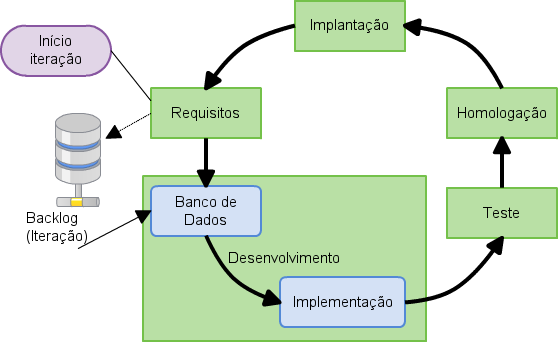
\includegraphics[scale=0.8]{figuras/ciclo_vida_solucao}
	\caption{Ciclo de vida da solução.}
	\label{ciclo_vida_solucao}
\end{figure}

A organização do ciclo de vida foi baseada na metodologia ágil \textit{Scrum}. A idéia básica desta organização é: definir o \textit{backlog} de um ciclo (\textit{backlog} da iteração) junto com o cliente, e então ir "consumindo" esse \textit{backlog} ao longo de todo o ciclo da solução, onde cada item do \textit{backlog} definido deverá caminhar sequencialmente pelas fases do ciclo de vida. Uma vez que todo o \textit{backlog} foi "consumido" pelo ciclo de vida, temos o fim de um ciclo ou iteração. Ao completar uma iteração, um novo \textit{backlog} é definido com o cliente, e então um novo ciclo se inicia. Esse fluxo se repete até que o sistema chegue ao nível desejado pelo cliente. As fases do ciclo de vida são descritas da seguinte forma:

\begin{itemize}
\item \textbf{Requisitos}: Priorizar as funcionalidades a serem desenvolvidas em um ciclo (\textit{backlog} da iteração) de acordo com os requisitos levantados junto com o cliente.
\item \textbf{Desenvolvimento}: Dividida pelas sub-fases Banco de dados e Implementação, esta fase tem o objetivo de realizar a construção do sistema. A sub-fase Banco de dados tem o objetivo de construir o modelo de dados, tanto lógico quanto físico. Já a sub-fase Implementação objetiva implementar de fato o sistema, baseado no modelo de dados construído.
\item \textbf{Teste}: Realizar os testes, tanto a nível de páginas da aplicação, quanto a nível de código, objetivando corrigir erros encontrados.
\item \textbf{Homologação}: Homologar a aplicação junto ao cliente e realizar a construção de materiais de apoio ao usuário, como guias, manuais, etc. Caso não seja homologada pelo cliente, o fluxo do ciclo volta para a fase que necessita de correções e passa por todas as etapas subsequentes, repetindo o ciclo.
\item \textbf{Implantação}: Planejar e realizar a migração do sistema para a produção.
\end{itemize}


Ao todo 18 atividades, 14 guias e 5 funcionalidades compõem a solução, onde os guias e as funcionalidades são suportes à execução de uma determinada atividade. A Figura \ref{atividades_solucao} ilustra a solução elaborada, agrupando todas as atividades, as funcionalidades e os guias, pelas fases do ciclo de vida. Os retângulos azuis representam as atividades e os retângulos roxos com laterais curvas representam os guias e as funcionalidades. Um guia ou uma funcionalidade representado após uma atividade significa que ele é um suporte a atividade em questão.
\clearpage

\begin{landscape}
\begin{figure}[!htb]
	\centering
		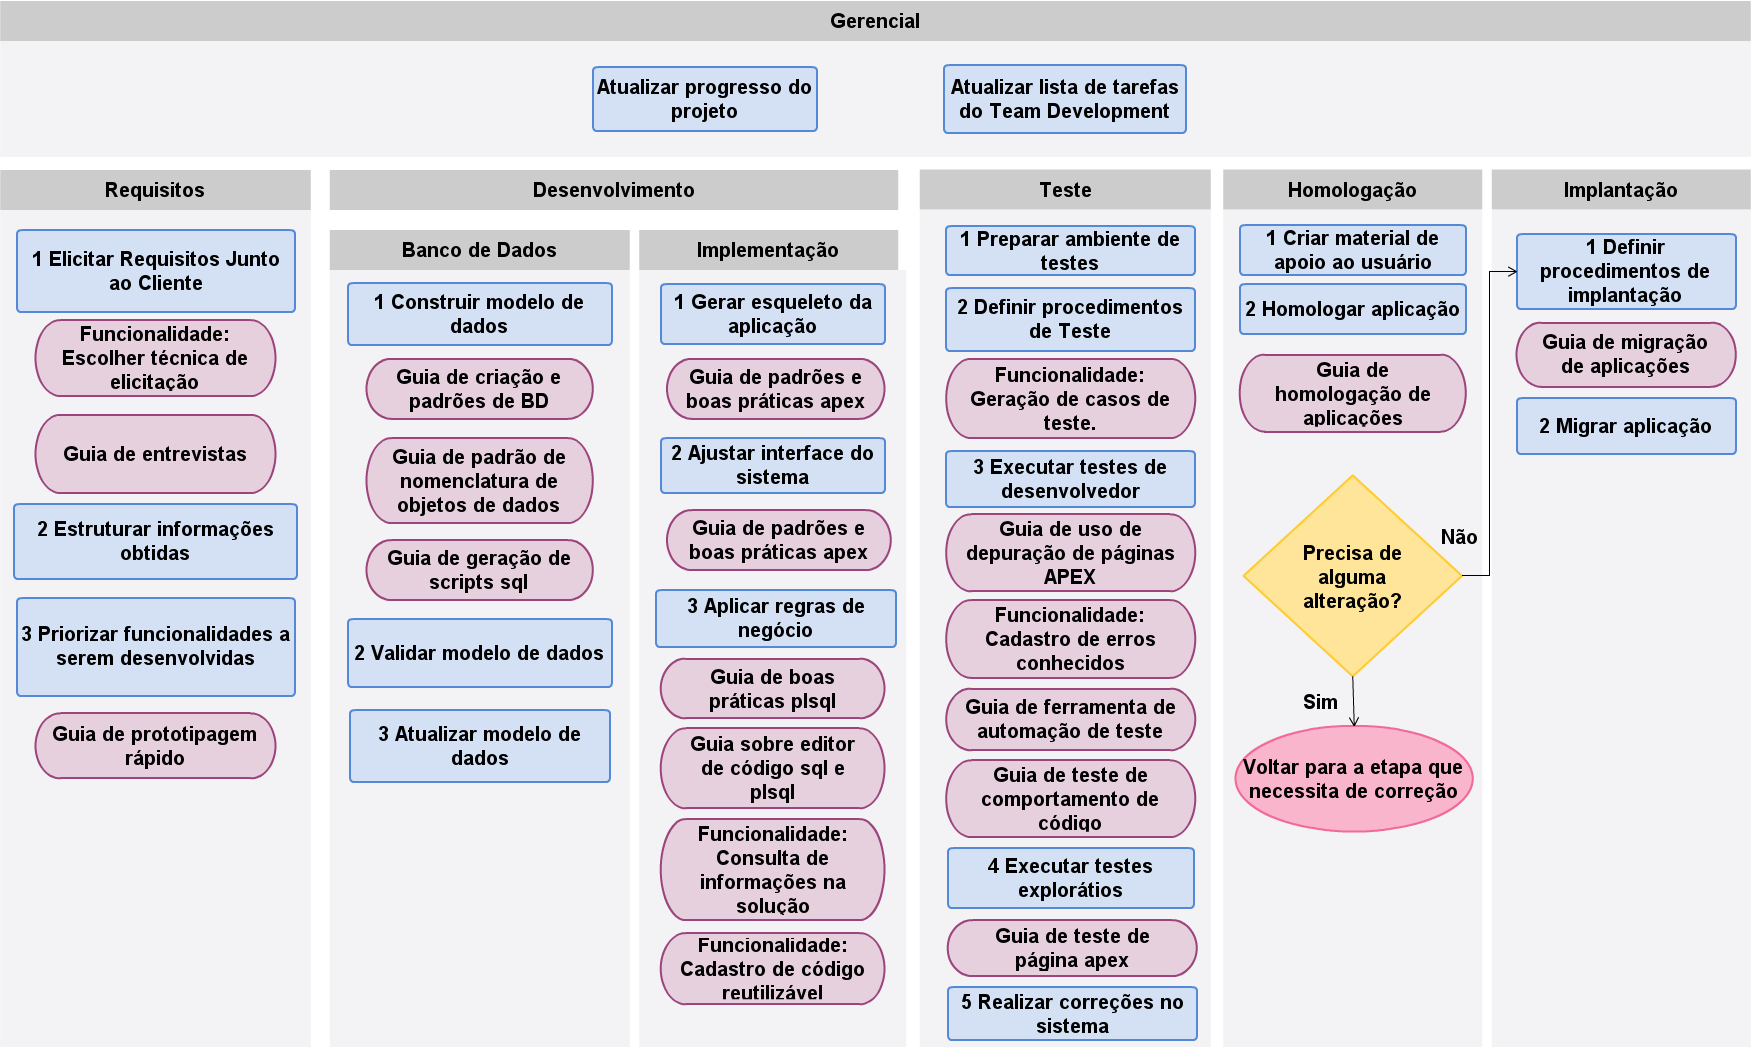
\includegraphics[scale=0.4]{figuras/fluxograma_solucao}
	\caption{Conjunto de atividades, guias e funcionalidades, por fase do ciclo de vida}
	\label{atividades_solucao}
\end{figure}
\end{landscape}

Nesta solução, o ponto de decisão na fase de homologação, representado pelo losango verde, indica se a execução do fluxo irá continuar ou se irá voltar a alguma atividade dentro de uma determinada fase. Esta atividade dependerá das solicitações feitas pelo cliente durante a atividade de "Homologar aplicação".

As atividades, guias e funcionalidades são descritas brevemente da seguinte forma:

\begin{itemize}
\item \textbf{Requisitos}
\begin{enumerate}
\item \textit{Elicitar Requisitos Junto ao Cliente (Atividade):} Identificar os requisitos funcionais e não funcionais da aplicação junto ao cliente.
\begin{enumerate}
\item \textit{Escolher técnica de elicitação (Funcionalidade):} Funcionalidade para ajudar o desenvolvedor a escolher uma técnica de elicitação para o levantamento de requisitos junto ao cliente. Uma técnica existente pré-cadastrada será sugerida ao usuário com base nas respostas de algumas perguntas.
\item \textit{Guia de entrevistas (Guia):} Guia de como elaborar perguntas para uma entrevista com o cliente. Este guia será útil somente para quem for utilizar a entrevista como técnica de elicitação.
\end{enumerate}
\item \textit{Estruturar informações obtidas (Atividade):} Transformar as informações obtidas na entrevista em requisitos, e armazená-los em documento.
\item \textit{Priorizar funcionalidades a serem desenvolvidas (Atividade):} Priorizar as funcionalidades a serem desenvolvidas dentro de um ciclo da solução.
\begin{enumerate}
\item \textit{Guia de prototipagem rápido (Guia):} Guia de como realizar uma prototipagem rápida das telas de uma aplicação.
\end{enumerate}
\end{enumerate}
\item \textbf{Desenvolvimento}
\begin{itemize}
\item \textbf{Banco de Dados}
\begin{enumerate}
\item \textit{Construir modelo de dados (Atividade):} Realizar a construção do modelo de dados lógico e físico.
\begin{enumerate}
\item \textit{Guia de criação e padrões de BD (Guia):} Guia com dicas de como realizar a modelagem conceitual (MER) e lógica (ML) do banco de dados da aplicação, utilizando a ferramenta Oracle Data Modeler. Utiliza o guia de padrão de nomenclatura de objetos de dados no auxílio da construção dos modelos.
%\begin{enumerate}
\item \textit{Guia de padrão de nomenclatura de objetos de dados (Guia):} Guia contendo os padrões de nomenclatura usados no órgão para diversos objetos do banco de dados, como tabelas, sequências, gatilhos e \textit{views}.
%\end{enumerate}
\item \textit{Guia de geração de scripts SQL (Guia):} Guia de como gerar os \textit{scripts} para a construção do modelo físico a partir do modelo lógico, elaborado na ferramenta Oracle Data Modeler.
\end{enumerate}
\item \textit{Validar modelo de dados (Atividade):} Realizar a validação do modelo de dados lógico e/ou físico, conforme a necessidade, com a área técnica responsável.
\item \textit{Atualizar modelo de dados (Atividade):} Atualizar o modelo de dados conforme as validações realizadas com a área técnica.
\end{enumerate}
\item \textbf{Implementação}
\begin{enumerate}
\item \textit{Gerar esqueleto da aplicação (Atividade):} Gerar o esqueleto da aplicação usando a funcionalidade \textit{defaults} de interface de usuário do APEX.
\begin{enumerate}
\item \textit{Guia de boas práticas APEX (Guia):} Guia para auxiliar a criação da aplicação usando boas práticas em APEX.
\end{enumerate}
\item \textit{Ajustar interface do sistema (Atividade):} Refinar a interface da aplicação conforme as necessidades de usabilidade da mesma.
\begin{enumerate}
\item \textit{Guia de boas práticas APEX (Guia):} Guia para auxiliar a criação da aplicação, usando boas práticas em APEX.
\end{enumerate}
\item \textit{Aplicar regras de negócio (Atividade):} Implementar as regras de negócio da aplicação.
\begin{enumerate}
\item \textit{Guia de boas práticas PL/SQL (Guia):} Guia para auxiliar a construção de código em PL/SQL.
\item \textit{Guia sobre editor de código SQL e PL/SQL (Guia):} Guia para auxiliar o uso do editor de código para a escrita de códigos SQL e PL/SQL.
\item \textit{Cadastro de código reutilizável (Funcionalidade):} Funcionalidade para permitir que o desenvolvedor possa cadastrar códigos que ele julgue ser reutilizáveis.
\end{enumerate}
\item \textit{Consulta de informações na solução (Funcionalidade):} Consulta conveniente das informações da solução, de forma a permitir um acesso mais rápido a um determinado guia ou funcionalidade. O usuário também pode cadastrar suas anotações. A idéia é semelhante a de uma \textit{Wiki}.
\end{enumerate}
\end{itemize}
\item \textbf{Teste}
\begin{enumerate}
\item \textit{Preparar ambiente de testes (Atividade):} Realizar os preparativos necessários ao ambiente para a realização dos testes da aplicação. Ex: Criar massa de dados, limpar dados existentes, criar um novo espaço de trabalho APEX, etc.
\item \textit{Definir procedimentos de teste (Atividade):} Definir um conjunto de etapas a serem realizadas nos testes.
\begin{enumerate}
\item \textit{Geração de casos de teste (Funcionalidade):} Funcionalidade que auxilie os testes do desenvolvedor, oferecendo diferentes valores que o usuário pode inserir nos diferentes componentes da interface, de forma a testar várias possibilidades diferentes.
\end{enumerate}
\item \textit{Executar testes de desenvolvedor (Atividade):} Executar os testes planejados.
\begin{enumerate}
\item \textit{Guia de uso de depuração de páginas APEX (Guia):} Guia explicando como usar a funcionalidade de depurar existente no APEX, para encontrar erros na aplicação.
\item \textit{Cadastro de erros conhecidos (Funcionalidade):} Funcionalidade que permita que o desenvolvedor possa cadastrar os erros que for encontrando, de forma a montar uma espécie de base de conhecimento de erros.
\item \textit{Guia de ferramenta de automação de teste (Guia):} Guia que auxilie o desenvolvedor a criar \textit{scripts} simples de automação de ações no navegador, de forma a criar testes automatizados.
\item \textit{Guia de teste de comportamento de código (Guia):} Guia que auxilie o desenvolvedor a testar, dentro do possível, o código PL/SQL e a realizar a depuração de códigos em PL/SQL.
\end{enumerate}
\item \textit{Executar testes exploratórios (Atividade):} Navegar na aplicação, sem um prévio planejamento, em busca de erros.
\begin{enumerate}
\item \textit{Guia de teste de página APEX (Guia):} Guia com dicas de como realizar os testes exploratórios.
\end{enumerate}
\item \textit{Realizar correções no sistema (Atividade):} Realizar as correções e ajustes necessários ao sistema.
\end{enumerate}
\item \textbf{Homologação}
\begin{enumerate}
\item \textit{Criar material de apoio ao usuário (Atividade):} Criar um guia que auxilie o usuário a usar a aplicação.
\item \textit{Homologar aplicação (Atividade):} Realizar a homologação da aplicação junto ao cliente.
\begin{enumerate}
\item \textit{Guia de homologação de aplicações (Guia):} Guia com dicas de como realizar a homologação junto ao cliente.
\end{enumerate}
\end{enumerate}
\item \textbf{Implantação}
\begin{enumerate}
\item \textit{Definir procedimentos de implantação (Atividade):} Definir as etapas necessárias para colocar a aplicação em produção.
\begin{enumerate}
\item \textit{Guia de migração de aplicações (Guia):} Guia com dicas do que se preocupar ao realizar a migração de uma aplicação APEX.
\end{enumerate}
\item \textit{Migrar aplicação (Atividade):} Executar os procedimentos de migração definidos.
\end{enumerate}
\clearpage
\item \textbf{Gerencial}
\begin{enumerate}
\item \textit{Atualizar progresso do projeto (Funcionalidade)}: Atualizar o progresso do projeto no quadro \textit{kanban} desenvolvido como uma funcionalidade da aplicação.
\item \textit{Atualizar lista de tarefas do Team Development (Atividade)}: Atualizar as tarefas registradas, conforme necessidade, na funcionalidade padrão do APEX, \textit{Team Development}.
\end{enumerate}
\end{itemize}

O esboço do quadro \textit{kanban} a ser elaborado na funcionalidade gerencial "Atualizar progresso do projeto", de forma a auxiliar o desenvolvedor na gerência do desenvolvimento, é apresentado na Figura \ref{kanban_criado}. \clearpage


\begin{landscape}
\vspace*{3cm}
\begin{figure}[!htb]
	\centering
		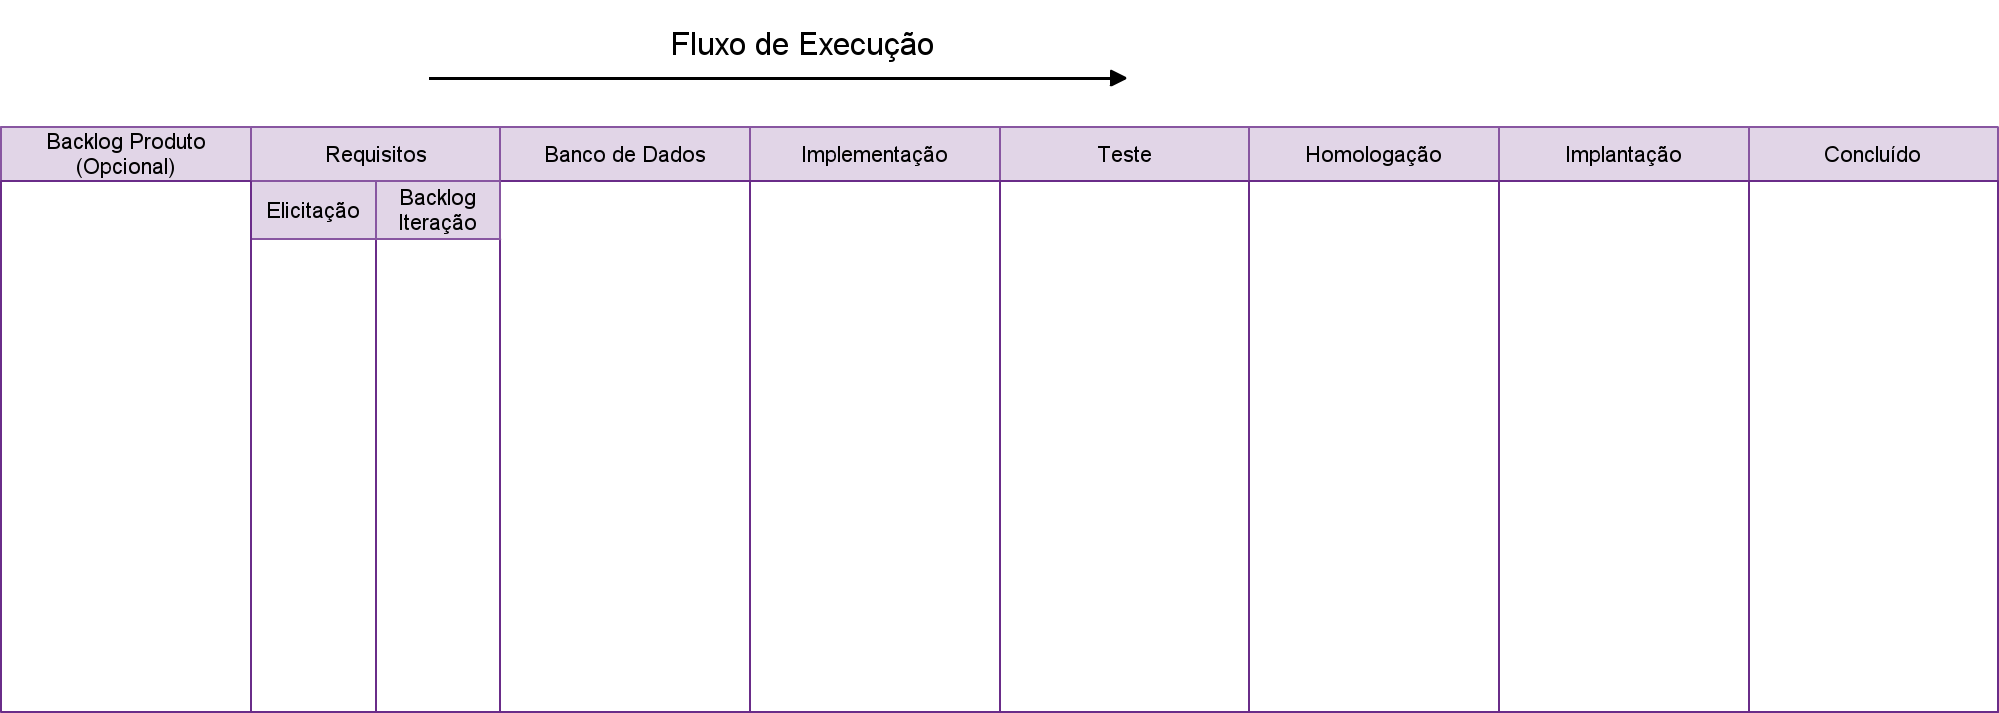
\includegraphics[scale=0.35]{figuras/kanban}
	\caption{Adaptação do quadro \textit{kanban}}
	\label{kanban_criado}
\end{figure}
\end{landscape}

Este quadro \textit{kanban} foi dividido pelas fases do ciclo de vida da solução, de forma que o desenvolvedor vai posicionando os itens do \textit{backlog} definido de acordo com a etapa em que se encontram dentro do ciclo de vida. A ideia é que o \textit{backlog} da iteração gerado seja em pequenas unidades de funcionalidades, de forma a facilitar o gerenciamento e acompanhamento pelo desenvolvedor. Ao terminar um conjunto destas unidades de funcionalidade, o desenvolvedor consegue gerar um software executável para o cliente. Observa-se que a divisão \textit{Backlog} Produto é opcional, já que pode ser da preferência do cliente e do desenvolvedor levantar o \textit{backlog} do produto. Porém, neste caso, o fluxo de execução do quadro \textit{kanban} obriga a seleção e priorização de um \textit{backlog} da iteração, conforme a divisão da etapa de Requisitos.

\section{SISADD - Sistema de Apoio ao Desenvolvimento Descentralizado}

O SISADD, Sistema de Apoio ao Desenvolvimento Descentralizado, é a implementação da solução gerada, desenvolvido na plataforma Oracle Application Express. As Figuras de \ref{tela_inicial_sisadd} a \ref{video_tutorial_sisadd} mostram as capturas das telas mais representativas do SISADD.

\begin{figure}[!h]
	\hspace*{-1.5cm} 
		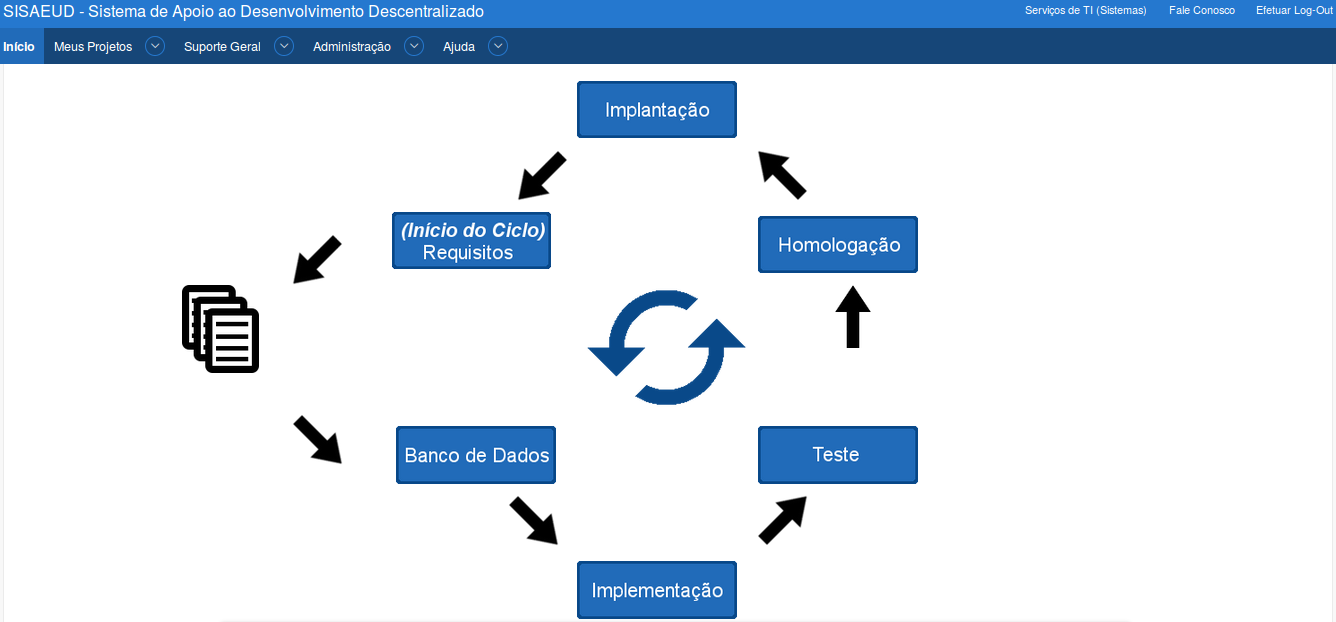
\includegraphics[scale=0.40]{figuras/home_p1}
	\caption{Tela inicial do SISADD}
	\label{tela_inicial_sisadd}
\end{figure}

Na tela inicial do SISADD é apresentado o diagrama do ciclo iterativo proposto para o desenvolvimento descentralizado, onde cada etapa deste ciclo é um botão clicável que o desenvolvedor pode usar para acessar o conjunto de atividades, guias e funcionalidades da respectiva etapa. Além disso, o menu superior oferece uma navegação mais rápida e direta para as funcionalidades da aplicação. Observa-se que este menu superior é apresentado em todas as telas do sistema.

A Figura \ref{ativ_guias_func_sisadd} ilustra um exemplo do detalhamento da etapa de requisitos, ou seja, é a tela apresentada caso o usuário clique na etapa de requisitos da tela da Figura \ref{tela_inicial_sisadd} (tela com o ciclo de desenvolvimento).

\begin{figure}[!htb]
	\hspace*{-1.5cm} 
		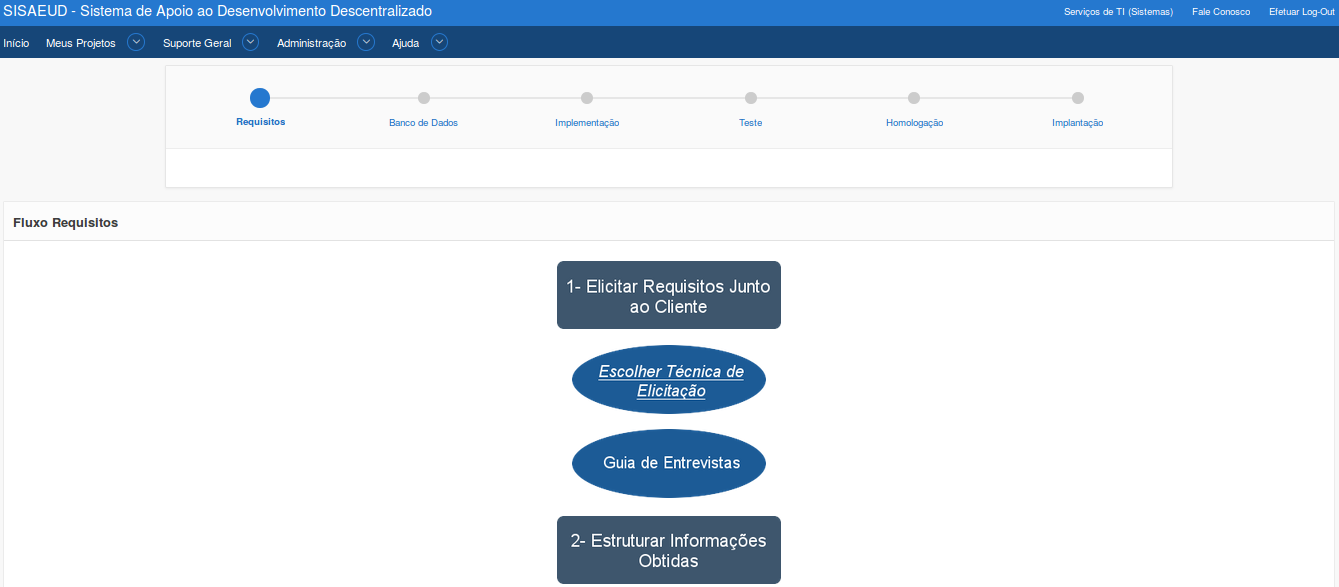
\includegraphics[scale=0.40]{figuras/fluxo_req_p2}
	\caption{Atividades, guias e funcionalidades da etapa de requisitos}
	\label{ativ_guias_func_sisadd}
\end{figure}

Dentro de cada etapa do ciclo temos um fluxo sequencial de atividades que são suportadas por um conjunto de guias e funcionalidades. Atividades são representadas por retângulos, guias são representados por elipses e funcionalidades são representadas por elipses com o texto sublinhado. Ainda nesta tela, a parte superior apresenta uma espécie de \textit{wizard}, onde cada etapa anterior a etapa na qual o desenvolvedor se encontra é marcada com um ícone de verificação, dando a entender que para estar nesta etapa o desenvolvedor teria que ter passado pelas etapas anteriores. %\clearpage

A Figura \ref{cadastro_projeto_sisadd} representa o cadastro de informações de um projeto, uma das mais importantes do sistema pois permite ao desenvolvedor cadastrar e editar informações a cerca do projeto no qual está trabalhando. \clearpage

\begin{figure}[!htb]
	\hspace*{-1.5cm} 
		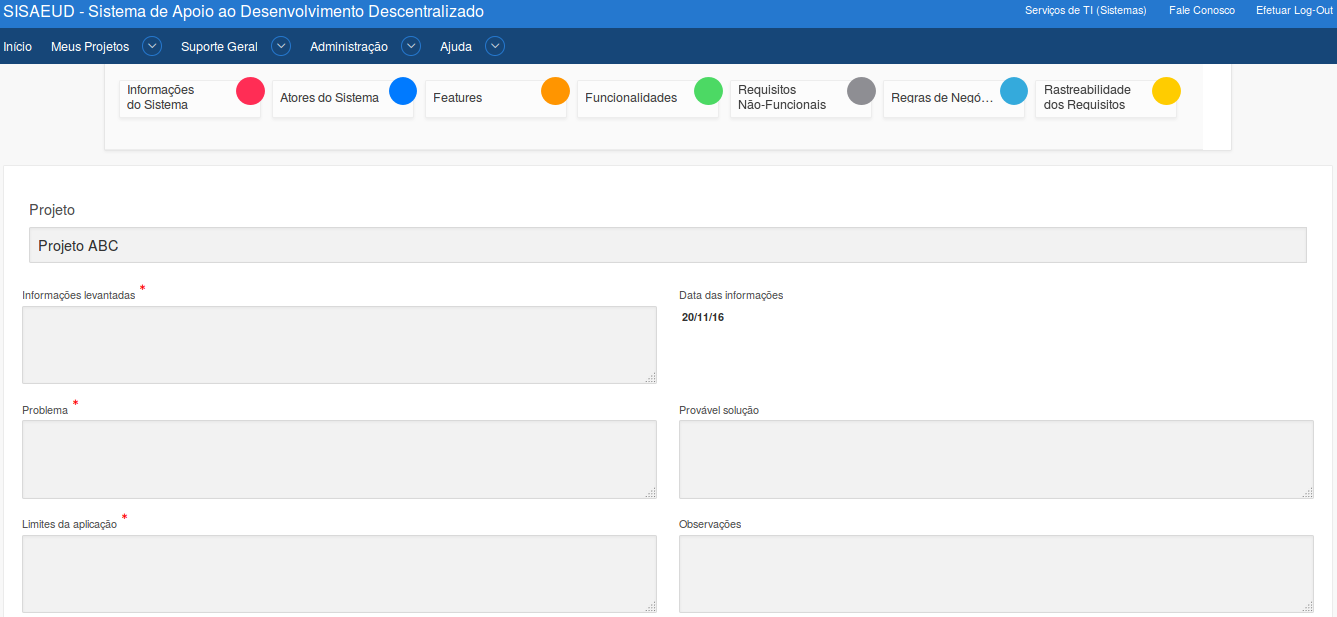
\includegraphics[scale=0.40]{figuras/cadastro_projeto_p14}
	\caption{Cadastro de informações de um projeto}
	\label{cadastro_projeto_sisadd}
\end{figure}

A parte superior exibe várias abas onde o desenvolvedor pode alternar entre várias telas de cadastro/edição de informações sobre o projeto, como: Informações do Sistema, Atores do Sistema, \textit{Features}, Funcionalidades, Requisitos Não Funcionais, Regras de Negócio e Visualizar a Rastreabilidade dos Requisitos.

A tela de geração de valores para teste do tipo caixa preta é representada pela Figura \ref{gerar_teste_sisadd} e esta funcionalidade gera um conjunto de valores para teste, seguindo o método BVA (\textit{Boundary Value Analysis}), de acordo com o componente selecionado.\clearpage

\begin{figure}[!htb]
	\hspace*{-1.5cm} 
		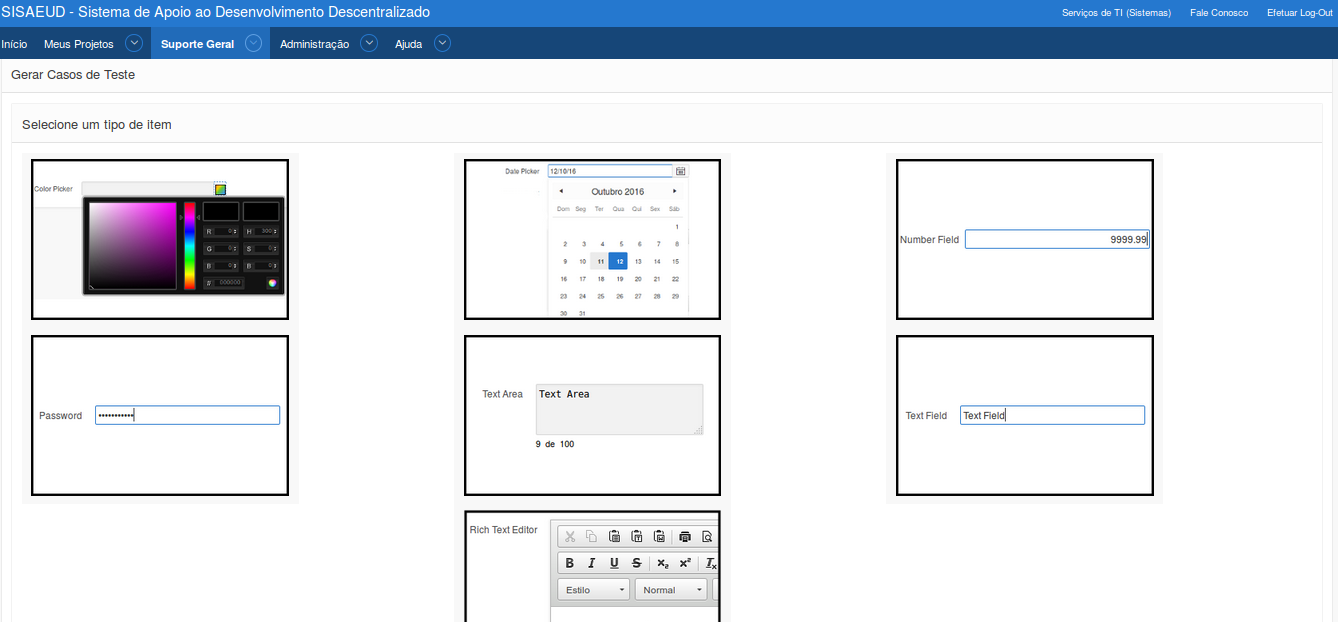
\includegraphics[scale=0.40]{figuras/gerador_teste_p57}
	\caption{Geração de valores para teste caixa preta}
	\label{gerar_teste_sisadd}
\end{figure}

Os componentes apresentados para escolha são componentes de entrada de dados disponíveis na versão 5 do APEX (versão mais atual). Desta forma, permite-se que o processo de teste do tipo caixa preta das páginas desenvolvidas seja mais sistemático.

A Figura \ref{guia_padrao_bd_sisadd} exibe o guia de padrão de nomenclatura de objetos de dados.

\begin{figure}[!htb]
	\hspace*{-1.5cm} 
		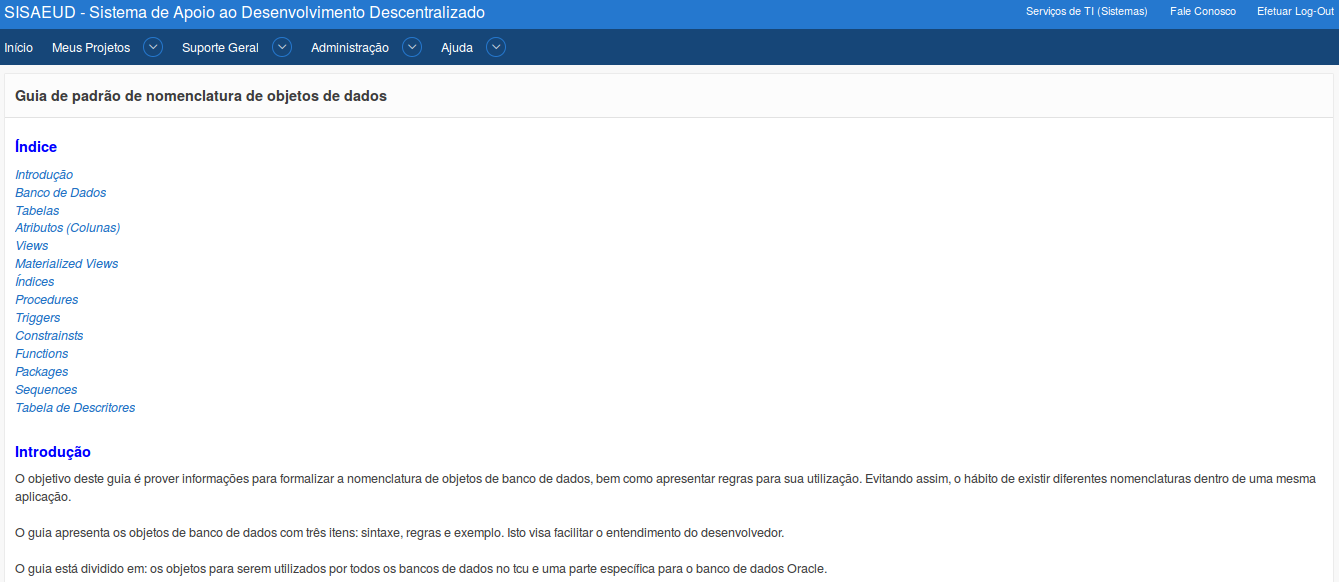
\includegraphics[scale=0.40]{figuras/guia_nomenclatura_bd_p54}
	\caption{Guia de padrão de nomenclatura de objetos de dados}
	\label{guia_padrao_bd_sisadd}
\end{figure}

O guia de padrão de nomenclatura de objetos de dados apresenta informações ao desenvolvedor de como nomear os objetos do banco de dados, de acordo com os padrões definidos pelo órgão público de estudo. Em todas as telas de guias são apresentados o índice, de forma a facilitar a navegação, seguido do conteúdo das seções.

Na Figura \ref{video_tutorial_sisadd} está ilustrado o \textit{player} de vídeo usado para a reprodução de vídeos tutoriais.

\begin{figure}[!htb]
	\hspace*{-1.5cm} 
		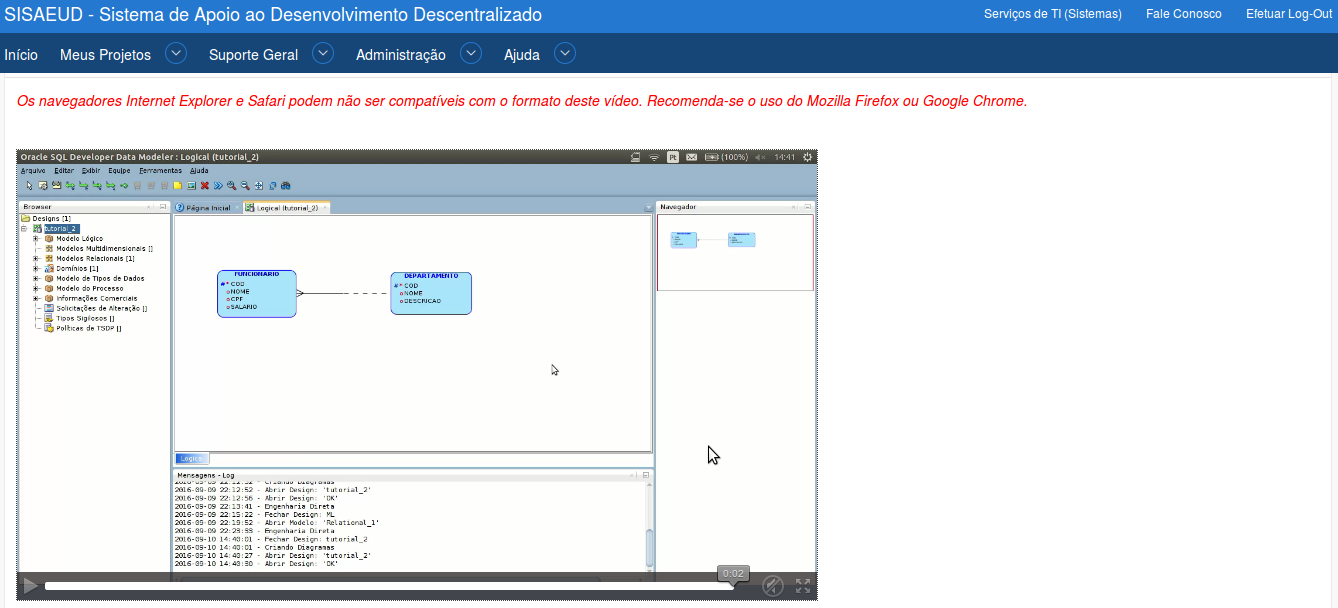
\includegraphics[scale=0.40]{figuras/video_p51}
	\caption{Vídeo tutorial de geração de modelo lógico de banco de dados}
	\label{video_tutorial_sisadd}
\end{figure}

Existem alguns guias que possuem um vídeo tutorial que foi gravado de forma a auxiliar o desenvolvedor. Para isso existe uma tela de reprodução de vídeo no formato WEBM (formato apropriado para vídeos em páginas web). O desenvolvedor pode executar todas as funções básicas de um \textit{player} de vídeo, como avançar, aumentar a tela e silenciar o vídeo.

\section{Análise Diagnóstico x Solução Implementada (SISADD)}

Para se ter uma noção do grau de conformidade que a solução implementada possui com o diagnóstico realizado, foi elaborada uma associação entre ambos. A Tabela \ref{diagnostico_x_solucao} apresenta a relação do diagnóstico obtido com o que foi implementado no SISADD. Observa-se que o diagnóstico obtido contém tanto problemas quanto algumas boas práticas e pontos positivos relatados pelos desenvolvedores entrevistados, na etapa de coleta de dados. As soluções pertencentes a coluna Implementação que contém um asterisco são soluções que até o momento não foram finalizadas ou que estão para ser iniciadas.

\begin{longtable}{|m{8.0cm}|m{8.0cm}|}
\caption{Diagnóstico Obtido x Solução Implementada}
\label{diagnostico_x_solucao}\\
\hline
\textbf{Diagnóstico} & \textbf{Implementação} \\
\hline
\endfirsthead
\hline
\textbf{Diagnóstico} & \textbf{Implementação} \\
\hline
\endhead
Curso da somente uma introdução                                                                                                   & \multirow{4}{*}{Consulta de Informações na Solução *}                                                                                                                                                      \\ \cline{1-1}
O curso poderia ser melhorado                                                                                                     &                                                                                                                                                                                                            \\ \cline{1-1}
Treinamento em boas práticas APEX                                                                                                 &                                                                                                                                                                                                            \\ \cline{1-1}
Construção de um catálogo de informações APEX                                                                                     &                                                                                                                                                                                                            \\ \hline
\multirow{3}{*}{Algumas aplicações com baixa qualidade}                                                                           & Guia de Padrões e Boas Práticas APEX                                                                                                                                                                       \\ \cline{2-2} 
                                                                                                                                  & Definir Procedimentos de Teste *                                                                                                                                                                           \\ \cline{2-2} 
                                                                                                                                  & Definir Procedimentos de Implantação                                                                                                                                                                      \\ \hline
Os requisitos são levantados através de reuniões.                                                                & \begin{tabular}{m{7.6cm}}- Priorizar Funcionalidades a Serem Desenvolvidas *\\- Elicitar Requisitos Junto ao Cliente\\- Guia de Entrevistas *\\- Escolher Técnica de Elicitação\end{tabular} \\
                                                                                                                                  &                                                                                                                                                                                                            \\ \cline{1-1}
\multirow{2}{*}{Reuniões constantes.}                                                                                             &                                                                                                                                                                                                            \\
                                                                                                                                  &                                                                                                                                                                                                            \\ \hline
Requisitos óbvios não anotados durante as reuniões são esquecidos                                                                 & \multirow{4}{*}{Estruturar Informações Obtidas}                                                                                                                                                            \\ \cline{1-1}
Registro de requisitos em papel                                                                                                   &                                                                                                                                                                                                            \\ \cline{1-1}
Registro de requisitos em sistemas distintos em rede                                                                              &                                                                                                                                                                                                            \\ \cline{1-1}
Registro de requisitos inexistente                                                                                                &                                                                                                                                                                                                            \\ \hline
Uso de prototipagem para levantar/validar requisitos                                                                              & Guia de Prototipagem Rápida                                                                                                                                                                               \\ \hline
Não atualiza o modelo de dados                                                                                                    & Atualizar Modelo de Dados *                                                                                                                                                                                \\ \hline
\begin{tabular}{m{7.6cm}}- Não valida o modelo de dados com área técnica\\- Valida o modelo de dados com área técnica\end{tabular} & Validar Modelo de Dados *                                                                                                                                                                                  \\ \hline
Possibilidade de gerar o modelo de dados a partir das tabelas                                                                     & Guia de Geração de Scripts SQL                                                                                                                                                                             \\ \hline
Negligência ao modelo de dados                                                                                                    & \begin{tabular}{m{7.6cm}}- Guia de Criação e Padrões, de BD\\- Guia de Padrão de Nomenclatura de Objetos de Dados\end{tabular}                                                                              \\ \hline
Elabora o modelo de dados utilizando ferramentas CASE                                                                             & Guia de Criação e Padrões, de BD                                                                                                                                                                           \\ \hline
\begin{tabular}{m{7.6cm}}- Realiza depurações no sistema com o APEX\\- Não realiza depurações\end{tabular}                         & \begin{tabular}{m{7.6cm}}- Guia de Uso de Depuração de Páginas APEX\\- Guia de Teste de Comportamento de Código *\end{tabular}                                                                              \\ \hline
Realiza depurações no console de comandos SQL                                                                                     & Guia de Teste de Comportamento de Código *                                                                                                                                                                 \\ \hline
Não há classificação de erros                                                                                                     & Cadastro de Erros Conhecidos                                                                                                                                                                               \\ \hline
Falta do uso de um padrão de boas práticas comprometeu a qualidade da aplicação        & \begin{tabular}{m{7.6cm}}- Guia de Padrões e Boas Práticas APEX\\- Guia de Boas Práticas PL/SQL *\\- Guia de Padrão de Nomenclatura de Objetos de Dados\end{tabular}                        \\ \cline{1-1}
Boas práticas realizada                                                                                                           &                                                                                                                                                                                                            \\ \hline
Escrita legível de código                                                                                                         & \begin{tabular}{m{7.6cm}}- Guia de Boas Práticas PL/SQL *\\- Guia de Padrão de Nomenclatura de Objetos de Dados\end{tabular}                                                                                \\ \hline
Mais da metade da aplicação é composta de algum código                                                                            & Guia de Boas Práticas PL/SQL *                                                                                                                                                                             \\ \hline
Preferência pelo uso de componentes padrões do APEX                                                                               & \multirow{2}{*}{Guia de Padrões e Boas Práticas APEX}                                                                                                                                                      \\ \cline{1-1}
Aplicação bem desenvolvida                                                                                                        &                                                                                                                                                                                                            \\ \hline
Falta de um padrão de boas práticas                                                                                               & \begin{tabular}{@{}l@{}}- Guia de Padrões e Boas Práticas APEX\\- Guia de Boas Práticas PL/SQL *\end{tabular}                                                                                              \\ \hline
Reutilização de código                                                                                                            & Cadastro de Código Reutilizável                                                                                                                                                                            \\ \hline
Uso de editores externos                                                                                                          & Guia Sobre Editor de Código SQL e PL/SQL *                                                                                                                                                \\ \cline{1-1}
Uso do editor do APEX                                                                                                             &                                                                                                                                                                                                            \\ \hline
Uso de testes funcionais                                                                                                          & \begin{tabular}{m{7.6cm}}- Geração de Casos de Teste\\- Guia de Ferramenta de Automação de Teste *\end{tabular}                                                                                             \\ \hline
Uso de teste de comandos SQL                                                                                                      & Guia de Teste de Comportamento de Código *                                                                                                                                                                 \\ \hline
Teste de execução de páginas                                                                                                      & Guia de Teste de Página APEX *                                                                                                                                                                             \\ \hline
Não há elaboração de casos de teste                                                                                               & Geração de Casos de Teste                                                                                                                                                                                  \\ \hline
Favorável à proposta de automação de testes funcionais                                                                            & Guia de Ferramenta de Automação de Teste *                                                                                                                                                                 \\ \hline
Costuma verificar se os apelidos não estão duplicados                                                                             & \multirow{3}{*}{Guia de Migração de Aplicações }                                                                                                                                                          \\ \cline{1-1}
Não migra as definições de objetos                                                                                                &                                                                                                                                                                                                            \\ \cline{1-1}
Verifica a criação das tabelas no espaço de produção                                                                              &                                                                                                                                                                                                            \\ \hline
Navegação feita, antes de migrar, somente nas páginas que alterou                                                                 & \multirow{3}{*}{Definir Procedimentos de Implantação }                                                                                                                                                    \\ \cline{1-1}
Navegação feita, antes de migrar, em todas as páginas da aplicação                                                                &                                                                                                                                                                                                            \\ \cline{1-1}
Faz a migração da definição dos objetos de dados                                                                                  &                                                                                                                                                                                                            \\ \hline
Faz a homologação das aplicações antes de disponibilizar definitivamente na produção  & \begin{tabular}{m{7.6cm}}- Homologar Aplicação *\\- Guia de Homologação de Aplicações *\end{tabular}                                                                                                        \\ \hline
\end{longtable}


Em relação ao diagnóstico temos um total de 44 itens distintos que contemplam problemas, boas práticas e pontos positivos. Deste total, 19 itens estão totalmente contemplados (concluídos) na implementação atual. Do restante, 9 itens estão parcialmente contemplados (parcialmente concluídos) e 17 itens não estão contemplados (implementação pendente de iniciar). Portanto temos os seguintes dados de conformidade do SISADD ao diagnóstico obtido:
\begin{itemize}
\item Conformidade total ao diagnóstico: Aproximadamente 43 \% (Totalmente contemplados);
\item Conformidade parcial ao diagnóstico: Aproximadamente 20 \% (Parcialmente contemplados);
\item Não contemplados: Aproximadamente 38 \%;
\item Conformidade geral (Total e Parcial): Aproximadamente 64 \%;
\end{itemize}

\begin{comment}
Apesar da conformidade geral ser de 64 \%, houveram implementações finalizadas que não estavam relacionadas ao diagnóstico obtido, ou seja, essas implementações foram levantadas com base na observação de pesquisa durante a construção da solução (descritas na Tabela \ref{features_estorias}).

Espera-se que o SISADD promova uma melhoria na qualidade e manutenibilidade das aplicações descentralizadas desenvolvidas, utilizando o Oracle APEX, no órgão público de estudo. Além disso espera-se que o SISADD seja utilizado em conjunto com outras formas de conhecimento já existente dentro do órgão, como a \textit{Wiki} do Desenvolvimento Descentralizado por exemplo. Nesse sentido ele passa a ser um complemento ao que já existe no órgão, o que permite que o conhecimento existente também possa ser utilizado.
\end{comment}

\chapter{Conclusão e Trabalhos Futuros}

A falta de de padrões e adesão a boas práticas no desenvolvimento de aplicações pode levar à problemas relacionados a qualidade e manutenibilidade das mesmas. Usuários finais não tem as mesmas habilidades e experiências de um desenvolvedor profissional. Portanto é necessário que esses desenvolvedores EUD tenham uma atenção especial para o desenvolvimento de suas aplicações, através de um modelo que lhes dê suporte. No órgão público de estudo o principal problema identificado está relacionado ao modo em que o desenvolvimento de sistemas descentralizados é executado, onde os departamentos desenvolvem os sistemas conforme suas necessidades e por isso geralmente acabam negligênciando o uso de boas práticas e padrões de desenvolvimento.

Tendo em vista o problema encontrado, este trabalho se propôs a desenvolver uma solução (sistema) de apoio ao desenvolvimento descentralizado no órgão público de estudo, agregando recursos que contribuam para a melhoria na qualidade e manutenibilidade dos sistemas desenvolvidos. A questão de pesquisa abordada é como apoiar o desenvolvedor na construção de sistemas descentralizados para promover a qualidade e manutenibilidade destes sistemas. Para responder a esta questão, foi realizada uma pesquisa explicativa com o uso do procedimento técnico bibliográfico, documental e pesquisa-ação participante. Desta forma o diagnóstico que identificou problemas, boas práticas e sugestões, do ponto de vista do desenvolvedor, foi realizado.

A partir do diagnóstico obtido e da análise de documentos do órgão, foi proposto o modelo de solução que contém o conjunto de atividades, guias de apoio e funcionalidades de forma a apoiar o desenvolvimento de sistemas. Este modelo então constituiu a base de requisitos para a implementação do sistema de apoio ao desenvolvimento descentralizado (SISADD) na ferramenta \textit{Oracle} APEX. Além da base de requisitos usada como insumo, houve o uso de observação por parte dos pesquisadores no contexto de atuação, o que permitiu uma abrangência maior na implementação do sistema.

\begin{comment}
Houveram dificuldades durante a implementação do sistema, tanto por conta de problemas com estimativas de esforço quanto por dependências de implementação que não puderam ser previstas de antemão. Além disso, o tamanho do escopo do trabalho foi um fator que contribuiu para que algumas implementações não pudessem ser realizadas ou ficarem pendentes. Um outro fator decisivo foi a questão da participação dos agentes envolvidos no contexto de atuação durante a implementação, o que fez com que a metologia abrangesse mais um procedimento técnico, a fim de dar maior autonomia de decisão aos membros do trabalho.
\end{comment}

Como trabalho futuro, é necessário a finalização da implementação da solução e a avaliação de sua efetividade em apoiar o desenvolvimento descentralizado dentro do órgão público de estudo. Esta avaliação deverá ser realizada com a escolha de um projeto piloto, a realização dos testes no mesmo e a coleta de resultados que indicam se o sistema atente ou não ao que foi proposto.